\documentclass[upright, contnum]{umemoria}
\deptoA{DEPARTAMENTO DE INGENIERÍA ELÉCTRICA}
\deptoB{DEPARTAMENTO DE CIENCIAS DE LA COMPUTACIÓN}
\author{Matías Fernando Pavez Bahamondes}
\title{Diseño e Implementación de Memoria de Largo Plazo para Robots de Servicio}
\auspicio{}
\date{2018}
\guia{Javier Ruiz del Solar, JOCELYN SIMMONDS WAGEMANN}
\carreraA{INGENIERO CIVIL ELÉCTRICO E}
\carreraB{INGENIERO CIVIL EN COMPUTACIÓN}
\memoria{MEMORIA PARA OPTAR AL TÍTULO DE INGENIERO CIVIL ELÉCTRICO E INGENIERO CIVIL EN COMPUTACIÓN}
\comision{Luis Mateu B., Andrés Caba}

\usepackage[T1]{fontenc}
\usepackage[spanish]{babelbib}
\usepackage{enumitem} % opciones para itemize 

% ------------- Imágenes -------------------------------------- %
\usepackage[pdftex]{graphicx}	% Para Archivos gráficos         %
\usepackage{float}				% Para usar H!                   %
\usepackage[section]{placeins}	% auto \FloatBarrier por sección %
\usepackage{caption}			% [font=small,labelfont=bf]      %
\usepackage{subcaption}         % Caption para subfiguras        %
\usepackage{sidecap}            % Captions al lado               %
\usepackage{wrapfig}            % Escribir alrededor             %
\graphicspath{{./figures/}}     % Agrega Path para buscar imgs.  %
% ------------------------------------------------------------- %

% = = = = = = = = = = = = = = = = = = = = = = =
% TODO NOTES
% = = = = = = = = = = = = = = = = = = = = = = =
\usepackage[pdftex,dvipsnames,table]{xcolor}  % Coloured text etc.
\usepackage[colorinlistoftodos,prependcaption,textsize=small]{todonotes}
%\usepackage[colorinlistoftodos,prependcaption,textsize=tiny,disable]{todonotes}
\newcommand{\todoimplementation}[1]{\todo[linecolor=blue,backgroundcolor=blue!25,bordercolor=blue,inline]{CODE ME: #1}}
\newcommand{\todopaused}[1]{\todo[linecolor=red,backgroundcolor=red!25,bordercolor=red,inline]{PAUSED: #1}}
\newcommand{\todounsure}[1]{\todo[linecolor=green,backgroundcolor=green!25,bordercolor=green,inline]{UNSURE: #1}}
\newcommand{\todojocelyn}[1]{\todo[linecolor=black,backgroundcolor=cyan!25,bordercolor=blue,inline]{CORRECCIÓN J.Simmonds: #1}}
\newcommand{\todomateu}[1]{\todo[linecolor=black,backgroundcolor=cyan!25,bordercolor=blue,inline]{CORRECCIÓN L.Mateu: #1}}
\newcommand{\todojavier}[1]{\todo[linecolor=black,backgroundcolor=cyan!25,bordercolor=blue,inline]{CORRECCIÓN J.Ruiz: #1}}
\newcommand{\todocaba}[1]{\todo[linecolor=black,backgroundcolor=cyan!25,bordercolor=blue,inline]{CORRECCIÓN A.Caba: #1}}
\newcommand{\todolater}[1]{\todo[linecolor=black,backgroundcolor=black!25,bordercolor=black,inline]{LATER: #1}}
\newcommand{\todofinal}[1]{\todo[linecolor=black,backgroundcolor=black!10,bordercolor=black,inline]{VERSION FINAL: #1}}
\newcommand{\todoimprove}[1]{\todo[linecolor=yellow,backgroundcolor=yellow!25,bordercolor=yellow,inline]{IMPROVEMENT: #1}}
\newcommand{\todowrite}[1]{\todo[linecolor=purple,backgroundcolor=purple!25,bordercolor=purple,inline]{WRITE ME: #1}}
\setlength{\marginparwidth}{0.5in} % mostrar correctamente todos al margen 
% = = = = = = = = = = = = = = = = = = = = = = =


\hypersetup{
	colorlinks,
	linkcolor={black},
	citecolor={blue!50!black},
	urlcolor={blue!80!black}
}

\usepackage{tikz}


%% Sections formatting
% -----------------------------------------

\usepackage{titlesec}
\usepackage[toc]{appendix}
\usepackage{etoolbox}
\makeatletter
% appendix and hyperref packages are broken with utf8!
% https://tex.stackexchange.com/questions/58848/ap%c3%a9ndices-appendix-spanish-accent
\appto{\appendices}{\def\Hy@chapapp{Appendix}}

% title sec is bugged on texlive-full deb. use this to correct it.
% Source: https://bugs.launchpad.net/ubuntu/+source/texlive-extra/+bug/1574052
\patchcmd{\ttlh@hang}{\parindent\z@}{\parindent\z@\leavevmode}{}{}
\patchcmd{\ttlh@hang}{\noindent}{}{}{}
\makeatother
% -----------------------------------------
% less spaced \paragraph sections
\titlespacing{\paragraph}{0pc}{0.0ex plus .1ex minus .2ex}{1pc}
%{12pc}{1.5ex plus .1ex minus .2ex}{1pc}

% Fancy chapters.. more on: https://ctan.org/pkg/fncychap
%Options: Sonny, Lenny, Glenn, Conny, Rejne, Bjarne, Bjornstrup, PetersLenny
\usepackage[Bjornstrup]{fncychap}

% Numbering and TOC for: 
% Chapters(0), Sections(1), subsections(2), subsubsections(3)
\setcounter{tocdepth}{2}
\setcounter{secnumdepth}{3}

% highlight
\usepackage{soul}
%\setulcolor{red}
%\sethlcolor{blue}
%\renewcommand\ul[1]{#1} % <<<<<<<<<<<<<<<<<<<<<<<<<<<<<<<<<<<<<
%\renewcommand\hl[1]{#1} % <<<<<<<<<<<<<<<<<<<<<<<<<<<<<<<<<<<<<


%%----- Colores --------------------------------------------------%
%\usepackage{color}												%
%\usepackage{colortbl}											%
%\usepackage[usenames,dvipsnames,svgnames,table]{xcolor}			%
%\definecolor{gray}{rgb}{0.51,0.51,0.51}							%
%\definecolor{dkgreen}{rgb}{0,0.6,0}								%
%\definecolor{mauve}{rgb}{0.58,0,0.82}							%
%%----------------------------------------------------------------%


% -------------------------------------------------------------------- %
% ----- LISTINGS ----------------------------------------------------- %
% -------------------------------------------------------------------- %
\usepackage{listingsutf8}

\renewcommand{\lstlistingname}{C\'odigo}
\renewcommand{\lstlistlistingname}{Listado de \lstlistingname s}

% --------------------------------------------------------%
% --------------- ESTILOS  -------------------------------%
% --------------------------------------------------------%
\lstdefinestyle{/Style/code}{
	%
	% ---- structure ----
	%title=\lstname,                    % show filename of files of title
	caption=\lstname,                   % also try caption instead
	captionpos=t,                       % caption-position to bottom
	basicstyle=\scriptsize\ttfamily,    % \footnotesize
	columns=fullflexible,               % %fixed
	tabsize=2,
	aboveskip={1.5\baselineskip},
	%
	% ---- numbers ----
	numbers=left,
	stepnumber=1,
	numbersep=5pt,                      % distance(line-numbers, code)
	numberstyle=\tiny\color{gray},      % for line-numbers	
	%
	% ---- shows ----
	showspaces=false,                   % spaces with particular underscores
	showstringspaces=false,             % underline spaces within strings
	showtabs=false,                     % tabs with particular underscores
	frame=false,                        % adds a frame around the code 
	%                                   % false, tb, shadowbox, single, lines
	%
	% ---- color ----
	backgroundcolor=\color{white},
	rulecolor=\color{black},
	%
	% ---- break ----
	breakatwhitespace=false,            % automatic breaks should only happen at whitespace
	breaklines=true,                    % automatic line breaking
	%                                   % Simbolo mostrado para el breakline
	prebreak = \raisebox{0ex}[0ex][0ex]{\ensuremath{\hookleftarrow}},
	%
	% ---- Extras ----
	%escapeinside={\%*}{*)},         	% LaTeX within your code
	extendedchars=true,
	inputencoding=utf8/latin1 			% Tildes
}

\lstdefinestyle{/Style/C}{
	language=C,
	keywordstyle=\bfseries\ttfamily\color[rgb]{0,0,1},
	identifierstyle=\ttfamily,
	commentstyle=\color[rgb]{0.133,0.545,0.133},
	stringstyle=\ttfamily\color[rgb]{0.627,0.126,0.941},
	style=/Style/code
}
\lstdefinestyle{/Style/C++}{
	language=C++,
	keywordstyle=\bfseries\ttfamily\color[rgb]{0,0,1},
	identifierstyle=\ttfamily,
	commentstyle=\color[rgb]{0.133,0.545,0.133},
	stringstyle=\ttfamily\color[rgb]{0.627,0.126,0.941},
	style=/Style/code
}

% --- XML de ROS ----------->
\lstdefinelanguage{/XML/ROS}{
	sensitive=false,
	morestring=[b]",
	%morestring=[s]{>}{<},
	morecomment=[s]{<!--}{-->},
	morecomment=[s]{<?}{?>},
	morekeywords={master, include, launch, node, param, rosparam, group, machine, arg} % list of attributes
}

\lstdefinestyle{/Style/XML/ROS}{
	language=/XML/ROS,
	stringstyle=\color{WildStrawberry},
	identifierstyle=\color{RoyalPurple},
	keywordstyle=\color{Emerald},
	%commentstyle=\color{Purple},	de los <? ?>
	commentstyle=\color{Blue},
	style=/Style/code
}
\lstdefinestyle{/Style/sh}{
	language=sh,
	stringstyle=\color{WildStrawberry},
	identifierstyle=\color{RoyalPurple},
	keywordstyle=\color{red},
	commentstyle=\color{Blue},
	style=/Style/code
}


% --- YAML de ROS ----------->
\newcommand\YAMLcolonstyle{\color{red}\mdseries}
\newcommand\YAMLkeystyle{\color{black}\bfseries}
\newcommand\YAMLvaluestyle{\color{blue}\mdseries}
\lstdefinelanguage{/YAML/ROS}{
    sensitive=false,
    morestring=[b]",
    morestring=[b]',
    moredelim=**[il][\YAMLcolonstyle{:}\YAMLvaluestyle]{:},
    morecomment=[l]{\#}
}
\lstdefinestyle{/Style/yaml/ROS}{
	language=/YAML/ROS,
	stringstyle=\color{Green},
	identifierstyle=\color{Black},
	keywordstyle=\color{Red},
	commentstyle=\color{Gray},
	style=/Style/code
}


% colores disponibles: https://en.wikibooks.org/wiki/LaTeX/Colors
% --- MSG de ROS ----------->
\lstdefinelanguage{/ROS/MSG}{
	%	alsodigit={-},
	alsoletter={},
	sensitive=true,
	comment=[l]{\#},
	keywords=[1]{
		uint32, uint8, string, float32, int32, bool, time,
		geometry\_msgs,Point,sensor\_msgs,Image
	},
	keywords=[2]{
		ltm, ltm\_samples, What, When, Where, Episode,
		Info, Date, Relevance, EmotionalRelevance, HistoricalRelevance
	},
	%otherkeywords={---,=}
}
\lstdefinestyle{/Style/ROS/MSG}{
	language=/ROS/MSG,
	stringstyle=\color{Green},
	identifierstyle=\color{Black},
	keywordstyle=[1]\bf\color{Red},
	keywordstyle=[2]\bf\color{Blue},
	commentstyle=\color{Gray},
	style=/Style/code
}

% --- JSON SAMPLE ----------->
\lstdefinelanguage{/MEM/JSON}{
	%	alsodigit={-},
	alsoletter={},
	sensitive=true,
	comment=[l]{\#},
	string=[s]{"}{"},
	keywords={\$in, \$or, \$gt},
}
\lstdefinestyle{/Style/JSON}{
	language=/MEM/JSON,
	stringstyle=\color{blue},
	identifierstyle=\color{Black},
	keywordstyle=\bf\color{Red},
	commentstyle=\color{Gray},
}


% custom caption for listings
\usepackage{caption}
\DeclareCaptionFont{listingfont}{\color{white}}
\DeclareCaptionFont{listinglabelfont}{\bf\color{white}}
\DeclareCaptionFormat{listing}{\colorbox{gray}{\parbox{\textwidth}{#1#2#3}}}
\captionsetup[lstlisting]{format=listing,labelfont=listinglabelfont,textfont=listingfont}


\begin{document}

\frontmatter
\maketitle

\begin{abstract}
\todolater{Abstract: Escribir al final.}
\end{abstract}

\begin{dedicatoria}
\todo[inline]{Escribir una dedicatoria corta}
\end{dedicatoria}

\begin{thanks}
\todo[inline]{Escribir agradecimientos}

% PÁRRAFOS
% - Conductor de bus que me atropelló... para tener más tiempo para trabajar en la memoria
% - La Innombrable por años de apoyo
% - Familia
% - Amigos .. partidas de hots... webeo diario para que trabaje en la cuestion
% - Homebreakers
% - Profesora Jocelyn Simmonds por sus correcciones y consejos.
% - ... JR por darme más y más pega, sin proveer consejos útiles.

\end{thanks}

\cleardoublepage
\tableofcontents
%\cleardoublepage
%\listoftables
%\cleardoublepage
%\listoffigures
%\cleardoublepage
%\lstlistoflistings

\listoftodos

\mainmatter

\todounsure{Agregar summary al final de cada capítulo?}


\chapter{Introducci\'on}

\section{Antecedentes Generales}

A continuaci\'on se presenta una breve introducci\'on a los temas requeridos para contextualizar este trabajo de t\'itulo: La rob\'otica de servicio y el equipo de trabajo donde se implantar\'a la soluci\'on. Adem\'as, se introduce el tema de la memoria humana, requerido para entender la propuesta y su relaci\'on con la rob\'otica.


\subsection{Robots de servicio}

La rob\'otica de servicio es un \'area enfocada en asistir a los seres humanos en tareas repetitivas y comunes, como la recolecci\'on de basura. Formalmente, se define un \textit{robot de servicio} como un robot ``que realiza tareas \'utiles para humanos o equipamiento, excluyendo aplicaciones de automatizaci\'on industrial''\cite{IFR}. Luego, el robot requiere cierto grado de autonom\'ia, que es la habilidad de actuar a partir del estado actual, usando lo que observa del ambiente y sin intervenci\'on humana. As\'i, un robot de servicio debe trabajar en ambientes no controlados y con la autonom\'ia suficiente que le permita llevar a cabo su cometido.

Un caso de uso t\'ipico es la asistencia en las tareas del hogar, donde se espera que un robot pueda ayudar a ordenar, preparar comida u ofrecer bebestibles. Otros casos de uso consideran el cuidado de adultos mayores, robots para compa\~nia en el hogar, mascotas robots, salud o educaci\'on. Particularmente, la compa\~nia SoftBank Robotics es pionera en ofrecer a Pepper como el primer robot humanoide ya adoptado en hogares de Jap\'on, as\'i como robot de bienvenida en hoteles y tiendas\cite{softbank}.


\subsection{Equipo de Trabajo: UChile Homebreakers}

El laboratorio de rob\'otica del Departamento de Ingenier\'ia El\'ectrica de la Universidad de Chile alberga dos equipos de rob\'otica: \textit{UChile Robotics Team}, dedicado al f\'utbol rob\'otico y \textit{UChile Homebreakers Team}, enfocado en rob\'otica de servicio. Ambos son conformados por alumnos de pregrado y postgrado de diversas especialidades, y liderados por el profesor Javier Ruiz del Solar\cite{uchile-robotics}.

UChile Homebreakers existe desde el a\~no 2007 y actualmente cuenta con 15 estudiantes. Todo su desarrollo de software est\'a basado en ROS, un framework para el desarrollo de plataformas rob\'oticas y con miles de usuarios alrededor del mundo\cite{ROS:2009}.

El equipo trabaja en dos plataformas humanoides, Bender y Pepper. Bender es un robot construido en el mismo laboratorio y con el objetivo de ser un mayordomo para el hogar. Pepper, desarrollado por SoftBank Robotics, est\'a dise\~nado para ser un robot de compa\~nia. Ambos comparten la misma arquitectura de software y pr\'acticamente todo su c\'odigo, exceptuando los drivers para acceder al hardware respectivo.


\subsubsection{RoboCup @Home League}


La RoboCup es una competencia internacional cuyo objetivo es ser un veh\'iculo para el desarrollo de la rob\'otica y la inteligencia artificial. Est\'a compuesta de variadas ligas: Rescue, Soccer, Simulation, @Home, Industrial y Junior, cada una con diversas subligas orientadas a fomentar la investigaci\'on de distintos aspectos del campo. Su sue\~no es que para mediados del siglo 21, un equipo de f\'utbol rob\'otico completamente aut\'onomo sea capaz de vencer al campi\'on de la \'ultima copa mundial y siguiendo las reglas de la FIFA\cite{robocup:rulebook_2017}.

UChile Homebreakers participa desde el a\~no 2007 en la categor\'ia @Home. Las pruebas de la liga se desarrollan en escenarios que imitan ambientes reales, como un hogar o un restaurante. 
%Adem\'as, la competencia funciona como un espect\'aculo para p\'ublico general, por lo que se priorizan pruebas y demostraciones interesantes para los espectadores.
% 
Las capacidades generalmente evaluadas y potenciadas en @Home son de Vision Computacional, Navegaci\'on aut\'onoma, Manipulaci\'on de objetos y Reconocimiento de Voz. Cada a\~no el equipo planifica sus desarrollos de acuerdo a los requerimientos de la competencia, por lo que trabajos fuera de las \'areas mencionadas no son considerados una prioridad.


\subsection{La memoria humana}

La memoria hace relaci\'on al almacenamiento de experiencias en el cerebro. Hay m\'ultiples sistemas de memoria independientes y sustentados por distintas estructuras cerebrales. A grandes rasgos, la memoria se puede dividir en de corto plazo STM (Short-Term Memory) y de largo plazo LTM (Large-Term Memory). La STM maneja informaci\'on muy detallada, es de poca capacidad y permite un r\'apido acceso, mientras que la LTM maneja mucha informaci\'on sobre experiencias y entidades, es menos detallada y de acceso m\'as lento\cite{Eichenbaum:2008}.

La LTM se puede dividir en expl\'icita (consciente) e impl\'icita (inconsciente). La primera almacena datos epis\'odicos, pudiendo responder las preguntas ``Qu\'e'', ``D\'onde'' y ``Cu\'ando'', datos sem\'anticos, que modelan hechos y conceptos como el lenguaje o personas, y tambi\'en, las conexiones entre ambas submemorias. La memoria impl\'icita codifica habilidades, h\'abitos y preferencias.

Existen procesos de consolidaci\'on y deterioro de la memoria que est\'an constantemente en funcionamiento. La consolidaci\'on requiere un est\'imulo relevante, sumado al proceso de almacenamiento, lo que genera conexiones entre la memoria epis\'odica y la respectiva zona sem\'antica. En caso de haber experiencias repetidas, las conexiones se fortalecen. El deterioro de la memoria es un proceso que degenera las conexiones entre ambas formas de memorias expl\'icitas.

La memoria emocional es una forma de memoria impl\'icita que genera reacciones emocionales y sentimientos. Seg\'un los est\'imulos a los que se enfrente, permite modular el proceso de consolidaci\'on de la STM en LTM, modificando el nivel de relevancia de los eventos, pudiendo generar memorias muy fuertes y h\'abitos arraigados. Ejemplos de esto son los flashbacks y las memorias asociadas a eventos importantes.



\section{Motivaci\'on}

La memoria es una habilidad cognitiva crucial para los humanos. Al interactuar con otras personas o el ambiente les permite recordar experiencias pasadas y sus detalles. Luego, es de esperar que un robot de servicio posea una memoria que le permita potenciar sus capacidades de interaci\'on con los humanos que ayudar\'a\cite{Vijayakumar2014}. Una LTM permitir\'ia, por ejemplo, generar di\'alogos interesantes sobre eventos pasados o cosas que el robot puede inferir del comportamiento humano, por otro lado, tambi\'en permitir\'ia la generalizaci\'on de las tareas que tiene que llevar a cabo.

Particularmente, dado el enfoque de las plataformas a utilizar, Bender c\'omo robot mayordomo y Pepper c\'omo robot social, se espera que ambos posean capacidades avanzadas de interaci\'on con los humanos, para lo que se requiere una LTM.


\subsection{Problema}

El a\~no 2015 se desarroll\'o una LTM epis\'odica para el robot Bender, orientada a la interacci\'on con personas y objetos\cite{Sanchez:2015}. El trabajo consideraba m\'etodos para almacenar, adquirir y manejar la informaci\'on epos\'odica, sumado a un proceso simple de consolidaci\'on de memoria.

Actualmente la memoria desarrollada no est\'a operativa, ni es factible habilitarla. A continuaci\'on se listan los aspectos que se consideran causas del problema desde un punto de vista t\'ecnico y humano:
\begin{itemize}
\item No se integr\'o adecuadamente al software del robot, no se recopila ni provee informaci\'on continuamente mientras el robot est\'a en funcionamiento.
\item La memoria no provee una API que siga el est\'andar de los desarrollos del equipo, por lo que no se usa ni es mantenida.
\item RoboCup@Home no considera el uso de LTM en sus competencias, por lo que el equipo no tiene un incentivo real para seguir desarrollando o mantener la memoria. Esto adem\'as ha provocado que el c\'odigo quede obsoleto.
\end{itemize}

Por otro lado, suponiendo que lo anterior estuviese solucionado, a\'un existen los siguientes problemas:
\begin{itemize}
\item S\'olo considera 2 modelos sem\'anticos: Persona y Objeto, para los cuales s\'olo se almacena informaci\'on de nombre, nacionalidad e imagen.
\item A pesar de considerar un modelo para objetos, no se integr\'o con los m\'odulos relacionados que recopilan la informaci\'on, por lo que realmente la memoria s\'olo funciona para entidades de tipo Persona.
\item Es esperable que una memoria considere m\'as modelos (Personas, Objetos, Autos, Ni\~nos, Mascotas, etc) y m\'as caracter\'isticas para cada modelo (nombre, hobbies, trabajo, etc).
\item La consolidaci\'on de memoria STM a LTM s\'olo considera la primera interacci\'on con cada entidad, por lo que no existe actualizaci\'on de los datos.
\item Hay una restricci\'on en los modelos y caracter\'isticas a almacenar, respecto a la informaci\'on que el robot es realmente capaz de obtener.
\end{itemize}


\subsection{Oportunidad}

Existe un vasto desarrollo respecto a la memoria y los procesos cognitivos, sin embargo, la investigaci\'on se concentra en campos como psicolog\'ia, neurolog\'ia y ciencias cognitivas. 
Los estudios de LTM para robots de servicio son muy acotados y no existe una soluci\'on est\'andar a implementar. Algunos robots, como la versi\'on comercial de Pepper, utilizan LTM, pero el c\'odigo asociado no es libre, ni est\'a basado en ROS.

El uso de LTM no est\'a en las prioridades ``RoboCup'' del equipo, sino que es algo \'util para demostraciones y para potenciar la interacci\'on humano-robot. Por ello, se considera que no basta con desarrollar un m\'odulo capaz de recopilar informaci\'on inteligentemente, sino que adem\'as se requiere una integraci\'on con las capacidades de di\'alogo o de inferencia de informaci\'on, para finalmente proveer una demostraci\'on de \'estas habilidades.

As\'i, \'esta es una oportunidad para dise\~nar una LTM para robots de servicio, que considere aspectos como: 
\begin{itemize}
\item Memoria epis\'odica y sem\'antica adecuada a tareas generales de robots de servicio.
\item M\'etodolog\'ia para consolidaci\'on de STM en LTM.
\item Servicio para recopilaci\'on continua de informaci\'on
\item Implementaci\'on est\'andar ROS, adecuada a las plataformas donde se implantar\'a la soluci\'on.
%\item Capacidad de generar respaldos de la memoria y recuperaci\'on de \'estos. 
\item Memoria emocional que permita dar relevancia a los eventos.
\item Inferencia de informaci\'on a partir de datos de la memoria. Por ejemplo: ``Juan suele desayunar a las 9am'', ``El control de la TV suele estar en el sof\'a'', etc.
%\item Integraci\'on con el di\'alogo que realiza el robot.\unsure{quitarlo?}
\end{itemize}

Tanto la memoria emocional, como la inferencia de informaci\'on, se consideran requisitos deseables, por lo que est\'an fuera del \textit{core} del proyecto.

%Tambi\'en se considera que es la oportunidad de promover la inclusi\'on de desafios basados en LTM en la liga @Home, a partir de los resultados de \'este trabajo. As\'i, el desarrollo de LTMs y capacidades asociadas dejar\'ia de ser postergado y pasar\'ia a ser una prioridad para los equipos de la competencia.


%\subsection{Aporte del Trabajo}
%La contribuci\'on del trabajo es principalmente el dise\~no e implementaci\'on 
\todo[inline]{Contribuci\'on del trabajo}

\section{Objetivos}

\subsection{Objetivo General}

El objetivo general corresponde al dise\~no de una LTM para robots de servicio, que considere componentes epis\'odicos y sem\'anticos. La LTM debe ser integrada en Bender y Pepper, con un servicio en background que recopile informaci\'on y con una API acorde a los desarrollos de UChile Homebreakers. Adem\'as, la LTM debe quedar integrada con alguna demostraci\'on de \'esta capacidad, ya sea mediante el di\'alogo o mediante inferencia de informaci\'on.

En resumen, el producto final debe ser una LTM integrada en los robots, de generaci\'on continua de recuerdos y que provea una demostraci\'on de \'esta capacidad.


\subsection{Objetivos Espec\'ificos}

A continuaci\'on se presentan los objetivos espec\'ificos del trabajo, a modo de desglose del objetivo general en tareas m\'as acotadas.

\begin{itemize}
\item Definici\'on del proceso de consolidaci\'on de recuerdos.
\item Dise\~no de la arquitectura del sistema y validaci\'on
\item Implementaci\'on de la LTM y su API.
\item Servicio para recopilaci\'on continua de informaci\'on.
\item Implementaci\'on de la demostraci\'on.
\end{itemize}

Otros objetivos espec\'ificos, correspondientes a requisitos que no son del \textit{core} del proyecto, son la implementaci\'on de la memoria emocional y la implementaci\'on de un m\'odulo de inferencia de informaci\'on basada en LTM.


%\section{Alcances}
\todo[inline]{ALCANCES}

%\section{Estructura de la memoria}
\todo[inline]{ESTRUCTURA DE LA MEMORIA1}

\chapter{Marco Teórico}\label{chapter:theory}

En este capítulo se revisan los temas y conceptos teóricos relevantes para el desarrollo del trabajo. Se formaliza la definición de robot doméstico y sus alcances. Se describe la memoria humana, sus categorías, funcionamiento y procesos cerebrales relevantes. Basado en los temas anteriores, se revisa la relación entre robótica y la memoria humana: se describen algunos enfoques existentes y las reglas generales para su implementación.

%% =====================================================================
\section{Robots de Servicio Domésticos}\label{sec:domestic_robots}
%% =====================================================================
%% =====================================================================
%% =====================================================================
%% =====================================================================

La Federación Internacional de Robótica (IFR)~\cite{IFR} define \textit{robot} como:
\begin{quotation}
	``Un mecanismo actuado y programable en dos o más ejes y con un cierto grado de autonomía, que se mueve en su entorno para realizar tareas previstas. En este contexto, autonomía se refiere a la habilidad de realizar tareas previstas, basado en el estado actual y lo sensado, sin intervención humana.''
\end{quotation}

Asimismo, la IFR define un \textit{robot de servicio} como un robot ``que realiza tareas útiles para humanos o equipamiento, excluyendo aplicaciones de automatización industrial''. Así, un robot de servicio debe trabajar en ambientes no controlados y con la autonomía suficiente que le permita llevar a cabo su cometido. Generalmente, la robótica de servicio se enfoca en asistir a los seres humanos en tareas repetitivas y comunes.

Según su área de aplicación, un robot de servicio se clasifica en \textit{de uso personal} o \textit{de uso profesional}. Los primeros son utilizados en ambientes no comerciales y por personas comunes; como por ejemplo, un robot sirviente o una silla de ruedas autónoma. Un robot de servicio profesional se utiliza en ambientes comerciales, usualmente operados por alguien entrenado; un ejemplo son los robots de entrega de paquetes o para cirugía.

Según la recopilación de datos realizada por la IFR durante el 2016, este tipo de robots es utilizado en diversas áreas para tareas domésticas, entretenimiento, educación, investigación, asistencia a ancianos y discapacitados, transporte, seguridad y vigilancia. Finalmente, existen otros robots de servicio que no pueden ser clasificados en las categorías anteriores.

El foco de este trabajo son los robots de servicio personales, dedicados a tareas domésticas, clasificación a la que en  adelante se referirá como \textit{robots domésticos}.


%% =====================================================================

%% =====================================================================

%% =====================================================================

%% =====================================================================

%% =====================================================================

%% =====================================================================

%% =====================================================================

%% =====================================================================

%% =====================================================================
\section{Memoria Humana}\label{sec:human_memory}
%% =====================================================================
%% =====================================================================
%% =====================================================================
%% =====================================================================

La memoria es un elemento fundamental para los humanos en su día a día, es parte integral de su existencia. Permite recordar quién, qué, cómo, dónde y cuándo. En términos psicológicos, es la habilidad para codificar, almacenar y luego obtener información sobre eventos pasados, en el cerebro. Los pensamientos son parte de la memoria de corto plazo, mientras que eventos pasados son almacenados en una memoria de largo plazo. Existen muchos estudios en el área de la psicología cognitiva con diversas descripciones y modelos teóricos de cada tipo de memoria~\cite{Vijayakumar2014}.

Desde el punto de vista de la información procesada, la memoria es vista como una facultad humana consistente en procesos para el manejo de información. Los 3 componentes principales son:

\begin{itemize}[topsep=0pt]
	\setlength\itemsep{0.2em}
	\item \textbf{Codificación}: En este paso, se adquiere nueva información desde los sentidos humanos. Los datos son convertidos a un formato que pueda ser almacenado en la estructura cerebral correspondiente.
	\item \textbf{Almacenamiento}: Consiste en la creación de registros permanentes de información. Es un proceso pasivo, de continuo procesamiento para clasificar datos nuevos y los ya existentes en el cerebro.
	\item \textbf{Adquisición}: Hace referencia al acceso de datos almacenados. El proceso se realiza en respuesta a una pista, que permita obtener una reconstrucción aproximada de la información, a partir de elementos repartidos en distintas partes del cerebro.
\end{itemize}
%\bigskip

La memoria puede ser dividida en múltiples sistemas independientes, con funcionalidades bien definidas y sustentados por distintas estructuras cerebrales~\cite{pmid-Squire}. La primera diferenciación define dos tipos de memoria: la de corto y la de largo plazo, STM (Short-Term Memory) y LTM (Long-Term Memory), por sus siglas en inglés~\cite{pmid10643472}. En el diagrama de la Figura~\ref{img:human_memory} se muestra una separación clásica utilizada en el área de las ciencias cognitivas~\cite{Eichenbaum:2008}, explicada en las siguientes subsecciones.

\usetikzlibrary{arrows,shapes,positioning,shadows,trees}
\tikzset{
	basic/.style  = {draw, drop shadow, font=\sffamily, rectangle},
	root/.style   = {basic, rounded corners=2pt, text width=10em, very thick, align=center, fill=gray!10},
	level 1/.style = {sibling distance=20mm},
	level 2/.style = {basic, rounded corners=6pt, thick,align=center, fill=gray!20, text width=8em},
	level 3/.style = {basic, rounded corners=2pt, thick, align=center, fill=gray!10, text width=6.5em},
	level 4/.style = {basic, thin, align=left, fill=gray!5, text width=10em}
}

\begin{figure}[!ht]
	\centering
	\begin{tikzpicture}[]
	
	\node [root] {Memoria Humana}
	child { node [level 2, xshift=-70pt] (c1) {\footnotesize Corto Plazo\\ (STM) }}
	child { node [level 2, xshift=100pt] (c2) {\footnotesize Largo Plazo\\ (LTM) }};
	
	\begin{scope}[every node/.style={level 3}]
	\node [below of = c2, xshift=-80pt, yshift=-20pt] (c21) {\footnotesize Explícita\\ (consciente)};  
	\node [below of = c2, xshift=80pt, yshift=-20pt] (c22) {\footnotesize Implícita\\ (inconsciente)};
	\end{scope} 
	
	\begin{scope}[every node/.style={level 4}]
	\node [below of = c21, xshift=40pt, yshift=-10pt] (c211) {\footnotesize Episódica};
	\node [below of = c211, xshift=0pt, yshift=0pt] (c212) {\footnotesize Semántica};
	
	\node [below of = c22, xshift=40pt, yshift=-10pt] (c221) {\footnotesize Procedural};
	\node [below of = c221, xshift=0pt, yshift=0pt] (c222) {\footnotesize Primado};
	\node [below of = c222, xshift=0pt, yshift=0pt] (c223) {\footnotesize Emocional};
	\end{scope} 
	
	\draw[-, to path={-- (\tikztotarget)}]
	(c2) edge (c21)
	(c2) edge (c22);
	
	\draw[-, to path={|- (\tikztotarget)}]
	(c21.195) edge (c211.west)
	(c21.195) edge (c212.west);
	
	\draw[-, to path={|- (\tikztotarget)}]
	(c22.195) edge (c221.west)
	(c22.195) edge (c222.west)
	(c22.195) edge (c223.west);
	
	\end{tikzpicture}
	\caption[Clasificaciones de la memoria humana.]
	{\small Clasificaciones de la memoria humana. Adaptado de~\cite{Vijayakumar2014}.}
	\label{img:human_memory}
\end{figure}



%% =====================================================================
%% =====================================================================
%% =====================================================================
\subsection{Memoria de corto plazo (STM)}
%% =====================================================================
%% =====================================================================
%% =====================================================================


En el ámbito cognitivo, la STM se refiere a la habilidad de estar atento, recopilar información  y memorias, para luego utilizarlas dentro de un corto periodo de tiempo~\cite{Eichenbaum:2008}. Es responsable de almacenar información constantemente y de decidir que parte será transferida a la LTM. El término de \textit{Memoria de Trabajo} suele ser utilizado de manera intercambiable con el de STM.

Se caracteriza por manejar información muy detallada, ser de poca capacidad y permitir un rápido acceso a estos datos. Permite recordar rápidamente y con gran detalle experiencias ocurridas hace pocos segundos, pero con dificultad creciente a medida que avanza el tiempo.

Se sustenta principalmente en la corteza prefrontal del cerebro. Las neuronas involucradas son capaces de mantener información relevante de corto plazo, la que es combinada con información sensorial entrante y áreas que manejan la toma de decisiones~\cite{Eichenbaum:2008}. 

En los humanos esta área presenta gran activación durante procesos de codificación, acceso y manipulación de memorias.


%% =====================================================================
%% =====================================================================
%% =====================================================================
\subsection{Memoria de largo plazo (LTM)}
%% =====================================================================
%% =====================================================================
%% =====================================================================


La LTM se asocia al almacenamiento permanente de información en el cerebro. Se caracteriza por manejar una gran cantidad de experiencias y entidades, ser menos detallada y proveer un acceso más lento a los recuerdos, respecto a la STM~\cite{Eichenbaum:2008}. Cierta información de la STM eventualmente es transferida a la LTM. De acuerdo a la Figura~\ref{img:human_memory}, sus dos principales categorías son la \textit{Memoria Implícita} y la \textit{Memoria Explícita}.


\subsubsection{LTM explícita}
%% =====================================================================

La memoria explícita suele ser denominada \textit{memoria consciente} o \textit{memoria declarativa}, pues maneja conocimientos relacionados a hechos y eventos adquiridos de forma consciente. Según las estructuras cerebrales involucradas, se conforma de la \textit{memoria episódica} y de la \textit{memoria semántica}~\cite{Eichenbaum:2008}.

La memoria episódica, por primera vez definida por Tulving~\cite{2_tulving}, es de carácter  autobiográfico y almacena detalles de eventos y experiencias pasadas. Permite responder a las preguntas ``Qué sucedió'', ``Dónde ocurrió'' y ``Cuándo ocurrió''~\cite{Deutsch2008}. Particularmente, se utiliza la noción de memoria episódica descrita por Clayton y Russel~\cite{CLAYTON20092330}, que incorpora el concepto de perspectiva episódica de los recuerdos. Un humano puede acceder a esta memoria si es capaz de decir: ``recuerdo que''. Este tipo de memoria da al ser humano la sensación de continuidad en el tiempo.

La memoria semántica almacena el conocimiento de hechos, significados, categorías y proposiciones. Un humano puede acceder a esta memoria si es capaz de decir: ``sé que''. Esta memoria se abstrae de perspectiva e información situacional.

Las estructuras cerebrales que soportan la memoria explícita son el hipocampo, encargado de manejar la memoria episódica, junto a la corteza cerebral, en donde se distribuyen los conocimientos de la memoria semántica. En el hipocampo se mantienen conexiones neuronales a los sectores de interés de la corteza, en donde se alojan conocimientos semánticos asociados a cada episodio.

Un ejemplo de uso de memoria episódica es el recuerdo de una graduación escolar, el lugar y la fecha donde ocurrió. La memoria semántica podría responder en que consiste una graduación y describir la ropa que se suele ocupar en ellas.



\subsubsection{LTM implícita}
%% =====================================================================

La memoria implícita abarca la capacidad de aprender habilidades, hábitos y preferencias, caracterizados por ser mejorados o adquiridos sin una recolección consciente. Así, también suele ser denominada \textit{memoria inconsciente} o \textit{memoria no declarativa}, pues comprende acciones que pueden ser realizadas sin pensar en ellas. Ejemplos de esto, son el andar en bicicleta o tocar un instrumento musical~\cite{Eichenbaum:2008}.

Dos de sus componentes son la \textit{memoria procedural} y la \textit{memoria de primado}. La primera ayuda a realizar tareas sin pensar en ellas, es decir, maneja el conocimiento del \textit{Cómo}; Ejemplos de esto son comer y caminar. La memoria de primado hace referencia a la predisposición para recordar hechos o información a la que un sujeto es expuesto con anterioridad; Ejemplos de esto son la facilidad para recordar canciones escuchadas hace poco tiempo, o el uso de palabras e ideas vistas recientemente.

Se ha mostrado que la memoria procedural se sustenta en el cerebelo, mediante la activación de este durante el uso de habilidades motoras.

Un tercer componente de la memoria implícita es la \textit{memoria emocional}. Esta se encarga de dar significado afectivo a ciertos estímulos, que de otra forma serían neutrales. Las estructuras cerebrales involucradas son la amígdala, las áreas corticales y subcorticales. Esta memoria se expresa mediante la activación del hipotálamo, en conjunto al sistema nervioso simpático, generando reacciones emocionales y sentimientos~\cite{episodic_philip}.


\subsection{Plasticidad sináptica y modulación}
%% =====================================================================

Se denomina \textit{consolidación} de memoria al proceso de transición de conocimiento desde la STM a la LTM~\cite{Bailey13445}. Durante la consolidación se generan conexiones neuronales entre la memoria episódica y la respectiva zona semántica. Para activar la consolidación se requiere de un estímulo relevante, sumado a la cadena de eventos para el almacenamiento~\cite{Eichenbaum:2008}.

Se denomina \textit{deterioro} de memoria u ``olvido'' al proceso de debilitamiento de las conexiones neuronales establecidas por los procesos de consolidación. Está en constante funcionamiento, degenerando las asociaciones entre la memoria episódica y la semántica. Por lo tanto, en este contexto, el olvido no significa una eliminación de los datos en el cerebro, sino que estos siguen ahí, pero la conexión requerida es inexistente o es demasiado débil para poder utilizarla.

Existen procesos químicos a nivel cerebral que afectan la consolidación y el deterioro de la LTM. Hay evidencia de que estos están en continuo funcionamiento. Estos eventos celulares ocurren en una escala de segundos a minutos, y son esenciales para la mantención de la LTM.

Es posible modular ambos procesos. Las experiencias repetidas potencian la consolidación de la memoria, lo que fortalece las conexiones neuronales. Por otro lado, la memoria emocional es capaz de potenciar o deprimir las reacciones químicas requeridas; según los estímulos a los que se enfrente, modifica el nivel de relevancia de los eventos, pudiendo generar memorias muy fuertes y hábitos arraigados. Ejemplos de esto, son la memorización por repetición, los flashbacks y las memorias asociadas a eventos importantes como cumpleaños.

%% =====================================================================

%% =====================================================================

%% =====================================================================

%% =====================================================================

%% =====================================================================

%% =====================================================================

%% =====================================================================

%% =====================================================================

\section{Memoria y Robótica}\label{sec:robotic_memory}
%% =====================================================================
%% =====================================================================
%% =====================================================================
%% =====================================================================
%% =====================================================================

En esta sección se revisan trabajos que buscan implementar LTM en robots. Se inicia haciendo énfasis en la importancia de esta en el campo de la robótica doméstica. Se hace una comparación entre la memoria humana y el manejo de información en robots. Luego, se revisan sistemas LTM encontrados en la literatura. Finalmente, se detallan las bases teóricas utilizadas para el diseño del proyecto, seleccionadas a partir de los trabajos más relevantes estudiados.


%% =====================================================================
%% =====================================================================
%% =====================================================================
\subsection{Relevancia de la LTM en robótica}
%% =====================================================================
%% =====================================================================
%% =====================================================================

% Ser Social e Interacciones
La LTM es una habilidad cognitiva esencial para cualquier ser social, otorgando una sensación de continuidad a la vida~\cite{Vijayakumar2014}. Durante una interacción social, permite recordar experiencias pasadas y relacionarlas con información actual, lo que genera interacciones interesantes y no monótonas. Lo mismo se aplica al caso de un robot doméstico, donde es esperable que posea una memoria que le permita establecer una relación de largo plazo con humanos, y potenciar sus capacidades de interacción con ellos.

% Robot SIN LTM
Para los desarrolladores, un problema común es que los usuarios tienden a perder el interés rápidamente en sus robots, pues existen expectativas no cumplidas respecto a la inteligencia y capacidad de socializar de la máquina~\cite{Ho2009}. El problema se potencia con el paso del tiempo, donde la motivación por interactuar disminuye y se genera frustración, a medida que el robot continua repitiendo los mismos comportamientos predefinidos. De manera similar para un humano, cuando la LTM no funciona correctamente debido a una enfermedad (por ejemplo, Alzheimer), la habilidad de interacción con otros humanos se ve dañada severamente~\cite{ltm_in_robocup}.

% Ventajas de LTM
Si se desea mejorar la interacción humano-robot, entonces se requiere que el robot se comporte de manera más natural. Los mejores agentes robóticos sociales deberían satisfacer las necesidades cognitivas y sociales humanas; mientras más familiar sea la interacción, serán más efectivos en su propósito. Así, la LTM es una habilidad crucial si se espera que el robot sea capaz de aprender y adaptarse a su entorno. Una LTM permitiría, por ejemplo, generar diálogos interesantes sobre eventos pasados o inferir aspectos del comportamiento humano, por otro lado, también permitiría la generalización de las tareas que tiene que llevar a cabo.

% Intentos
Durante la última década han habido algunos intentos de implementar LTM en robots domésticos, sin embargo, no existe una solución estándar y aún quedan muchas consultas sin responder~\cite{ltm_in_robocup}. Por ejemplo, no existe una estrategia clara para el almacenamiento de eventos y experiencias en la forma de episodios en una memoria LTM. Tampoco está claro como almacenar el estado emocional del robot y utilizarlo para modulación de la relevancia episódica. Otros puntos en investigación son la forma de consolidar la STM en LTM, la implementación de mecanismos de olvido y represión, y como manejar los aspectos éticos de adquirir y almacenar información personal de usuarios.

% Historias de Éxito
Por otro lado, desde un punto de vista práctico, se ha mostrado que el concepto de memoria LTM aplicada a robots es beneficioso. Salgado et al.~\cite{Salgado2012} ocupan memoria procedural para mejorar el desempeño de un robot en ambientes dinámicos, logrando acelerar el proceso de adaptación al entorno y la toma de decisiones.


%%% =====================================================================
%%% =====================================================================
%%% =====================================================================
%\subsection{Relación entre la memoria humana y la memoria robótica}
%%% =====================================================================
%%% =====================================================================
%%% =====================================================================
%
%Son muchos los trabajos en LTM que han basado su desarrollo en la taxonomía de la memoria humana, donde se implementan esquemas de información con módulos análogos a los presentados en la Figura~\ref{img:human_memory}. Esto se puede justificar por la similitud de cada tipo de memoria, con módulos preexistentes en la arquitectura robótica. A continuación se presenta una comparación entre cada tipo de memoria, sus procesos y el análogo robótico.
%
%\subsubsection{Memoria STM}
%Se relaciona a todos los datos que están actualmente cargados en la memoria primaria de la máquina. Esta memoria es la utilizada para solucionar la tarea actual, es equivalente a los pensamientos del robot y cumple con las características de la STM humana: es volátil, de rápido acceso y limitada en capacidad. También se encuentra presente en todo archivo temporal manejado por el sistema, mientras está en funcionamiento. Así, la estructura equivalente a la cerebral sería principalmente la RAM de la máquina y los archivos temporales.
%
%\subsubsection{Memoria Semántica}
%La memoria semántica es común y se puede asociar a casi toda fuente de datos estática, no utilizada por las otras memorias. Luego, la memoria semántica se sustenta en la memoria secundaria, cumpliendo las características de su análogo en los humanos: es persistente, de acceso costoso y virtualmente ilimitada en capacidad. En general, todo archivo con datos persistentes, utilizados para el funcionamiento del robot se podría considerar en esta categoría. Algunos ejemplos son:
%\begin{itemize}
%	\item Bases de datos.
%	\item Directorios con imágenes de personas y objetos conocidos.
%	\item Mapas con descripción del ambiente.
%	\item Archivos de audio utilizados por el robot.
%\end{itemize}
%
%
%\subsubsection{Memoria Procedural}
%Este tipo de memoria es comparable a algoritmos predefinidos para realizar acciones, generalmente motoras. Las estructuras equivalentes a la versión cerebral serían los archivos con parámetros para cada algoritmo, obtenidos a partir del entrenamiento o ajustados manualmente. Algunos ejemplos comparables son: 
%\begin{itemize}
%	\item Algoritmos basados en redes neuronales, entrenados para manipular objetos o reconocer patrones.
%	\item Algoritmos entrenados para tareas específicas, cómo la detección de caras o el reconocimiento de voz.
%	\item Controladores basados en puntos de operación para acciones motoras.
%	\item Síntesis de voz.
%\end{itemize}
%
%
%\subsubsection{Otros tipos de memoria}
%Generalmente, las memorias STM, semántica y procedural son un requisito mínimo para el funcionamiento de un software robótico, pero no son implementadas de forma explícita, sino que se pueden identificar en los componentes de software descritos anteriormente. Luego, la existencia de tales memorias, no implica la intención de crear una arquitectura LTM similar a la humana. Los otros tipos de memorias solo son implementados en casos especializados.
%
%

%% =====================================================================
%% =====================================================================
%% =====================================================================
\subsection{Revisión de sistemas LTM}\label{sec:revision_LTM}
%% =====================================================================
%% =====================================================================
%% =====================================================================
% - frameworks
% - trabajos relacionados
% - otros aspectos

A continuación se presenta una revisión de sistemas LTM basados en la memoria humana. En primer lugar se describen otras implementaciones de estos sistemas. Luego, se estudian trabajos con aspectos de interés para un sistema LTM. Para concluir, se muestran algunos trabajos enfocados en aspectos interesantes, pero que escapan de los alcances del proyecto.

\subsubsection{Frameworks LTM}

\ltmconcept{SOAR-EM (2004)} 
% Más info en: Sanchez:2015 , Stachowicz2012 , Deutsch2008
% About
Nuxoll y Laird presentaron SOAR-EM~\cite{Nuxoll2004ACM}, una extensión con memoria episódica para la arquitectura SOAR~\cite{LAIRD19871}. Ellos desarrollaron un sistema similar a PACMAN, donde la máquina debe moverse a través de una grilla para buscar ``comida'' lo más rápido posible. Utilizaron la memoria episódica para dar apoyo en la planificación de los movimientos del agente, mostrando que aquellos equipados con memoria episódica tienen un mejor desempeño que los que carecen de ella. 

% Episodios y limitantes
En SOAR-EM un episodio es creado con datos de la STM por cada acción del agente, los que pueden ser recolectados a partir de una pista episódica. Sin embargo, más adelante se mostró que el mecanismo de recolección es ineficiente y difícil de optimizar~\cite{Nuxoll2007}. Por otro lado, el trabajo no considera aspectos como el olvido episódico, ni la interacción de emociones con la LTM.


\ltmconcept{ISAC (2005)}
% Más info en: Sanchez:2015 , Stachowicz2012 , Deutsch2008
En el año 2005 Ratanaswasd et al.~\cite{Ratanaswasd2005} agregan memoria episódica al robot humanoide ISAC (Intelligent Soft Arm Control), enfocado en la manipulación de objetos. Los episodios son almacenados por su fecha y hora, combinados con todos los contenidos semánticos que aparecen en ese lapso. Luego, estos son recolectados para soportar la toma de decisiones en la planificación de trayectorias robóticas, bajo la suposición de que siempre existirá un episodio lo suficientemente similar a la situación actual. Más tarde, Dodd y Gutierrez~\cite{Dodd2005} incorporaron el concepto de relevancia emocional e histórica, con el objetivo de optimizar la búsqueda y eliminación de eventos según su intensidad. La relevancia emocional se obtiene directamente desde el sistema emocional de ISAC. Para la relevancia histórica, los eventos recientes son más importantes que los pasados, y experiencias novedosas tienen mayor puntaje que las comunes.

Los datos almacenados cubren el Qué, Cuándo y Dónde requeridos por Clayton~\cite{CLAYTON20092330}. Sin embargo, el diseño no provee la flexibilidad esperada en un sistema de memoria episódica:  Delimita los episodios por cambios en los objetivos generales de planificación del robot. No soporta el traslape ni la anidación de eventos. No queda claro si es suficientemente eficiente o escalable para cumplir con los requerimientos de un sistema episódico~\cite{Stachowicz2012}.

\ltmconcept{EPIROME (2008)} 
% Más información en:~\cite{Sanchez:2015}, Stachowicz2012
TASER es un robot de servicio enfocado a ambientes reales de oficina~\cite{Jockel2007}. Jockel et al.~\cite{Jockel2008} proponen el uso de memoria episódica para apoyar con tareas y evitar trabajo innecesario. Por ejemplo, al revisar oficinas para ayudar buscando personas, podría evitar las que usualmente están vacías. Para ello, Jockel et al. desarrollaron el framework EPIROME. Sus simulaciones mostraron que los agentes con memoria episódica se adaptan más rápido a nuevas situaciones que aquellos que carecen de ella.

A partir sus características, EPIROME no cumple con los requerimientos de un sistema de memoria episódica: No dispone de almacenamiento de largo plazo, mecanismos de recolección de episodios, ni representaciones de los eventos almacenados~\cite{Stachowicz2012}.

\ltmconcept{ALIZ-E (2014)}
ALIZ-E (Adaptative Strategies for Sustainable Long-Term Social Interaction) es un sistema cognitivo enfocado en la interacción natural con niños. Vijayakumar desarrolló una extensión de memoria episódica para ALIZ-E, basado en el funcionamiento de la memoria humana~\cite{Vijayakumar2014}. Su módulo construye episodios en formato RDF (Resource Description Framework), a partir de los archivos de \textit{log} que genera el sistema tras cada interacción.

Vijayakumar muestra que su sistema cumple con los requisitos de eficiencia esperados para su plataforma objetivo. Sin embargo, no aborda el diseño de metodologías para adquisición de episodios, ni la definición de información semántica, pues se enfoca en adaptar los archivos de \textit{log} preexistentes. Por otro lado, propone un caso de uso interesante para un robot social, a través de la adaptación de sus frases, según la información episódica almacenada, e.g., cambiando la frase ``Estoy feliz de verte'' a ``Estoy feliz de verte \textit{nuevamente}''. 


\ltmconcept{Bender}
El año 2015 Sanchez et al.~\cite{Sanchez:2015} diseñaron un sistema de memoria episódica para el robot Bender (plataforma de este proyecto). Este primer acercamiento es descrito en detalle en la Sección~\ref{sec:primer_acercamiento} y es utilizado como parte de la motivación para este proyecto.


\ltmconcept{Otros trabajos}
Existen otros esfuerzos en equipar robots con memoria episódica, por ejemplo, MINERVA2~\cite{Douglas1988}, LIDA~\cite{Feinstone2006}, Rity~\cite{Kuppuswamy2006}, Homer~\cite{Vere1990} y personajes de historias virtuales~\cite{Brom2007}. De manera similar a los trabajos descritos anteriormente, la mayoría de estos sistemas ha sido diseñado para satisfacer un contexto particular, por lo que no son útiles para el diseño de nuevos sistemas cognitivos robóticos~\cite{Stachowicz2012}.

% -~\cite{Pratama2014} ??
% - MINERVA 2 (1988)~\cite{Douglas1988}.  Más información en~\cite{Jockel2008}.
% - LIDA (2006)~\cite{Feinstone2006} % Más información:~\cite{Jockel2008}
% - Tecuci (2005)  % Más información: Deutsch2008
% D. Tecuci, “A generic episodic memory module,” University of Texas at Austin, Tech. Rep., 2005.D. Tecuci, “A generic episodic memory module,” University of Texas at Austin, Tech. Rep., 2005.



%\todoimprove{Agregar tabla indicando pros/cons de cada sistema LTM}


%\subsubsection{Procesos de consolidación y deterioro}
%
%%%- algunos solo procuran desarrollar reglas sobre como actualizar los pesos de aprendizaje
%% - dejar de aprender (sorprenderse al ser mayor)
%% - si no se implementa olvido, entonces la busqueda de informacion seria cada vez mas compleja.~\cite{Deutsch2008}
%
%
%%\todounsure{Hablar sobre este paper: sueño y postprocesamiento, puede estar demás para el marco teórico...}
%
%En un esquema LTM, un episodio puede estar constituido de muchos eventos, pero no todos son igualmente relevantes. En su trabajo, Kelley~\cite{Kelley2014} estudia 3 estrategias para la consolidación de recuerdos. La primera almacena todos los eventos ocurridos, pero tiene un costo de búsqueda lineal, respecto a los eventos almacenados; esta estrategia es impráctica a largo plazo. La segunda solo almacena eventos interesantes y realiza una búsqueda entre los más recientes; esta estrategia es práctica, pero no permite abstracción del evento. La tercera estrategia se basa en un postprocesamiento de las memorias, de manera similar al sueño humano.
%
%La estrategia propuesta por Kelley se basa en recordar todos los eventos, pero realizando un postprocesamiento de los datos una vez terminado el episodio. La ventaja es que no solo permite recordar los eventos interesantes del episodio, sino que además permite reconocer pistas o estímulos previos que sirven para prevenir un evento indeseado o potenciar eventos interesantes. Además, permite almacenar eventos posteriores, que sirven para entender las consecuencias del evento de interés. 
%
%En la Figura~\ref{img:sleep_eventos} se muestra un episodio conformado de una secuencia de 9 eventos. Entre los marcadores 1-2 y 5-6 hay eventos considerados poco interesantes, mientras que los eventos entre 3-4 son interesantes. Kelley propone almacenar la secuencia completa de eventos, para descartar los que no son útiles en un postprocesamiento. A priori se deben quitar los eventos entre 1-2 y 5-6, sin embargo, el evento 2 se mantiene en la memoria episódica como pista, y el evento 5 se mantiene para reforzar la consecuencia del episodio. Los resultados se pueden utilizar para aprendizaje reforzado, mientras que las pistas sirven para generalizar el episodio, en caso de que sean recurrentes.
%
%\begin{figure}[!ht]
%	\centering
%	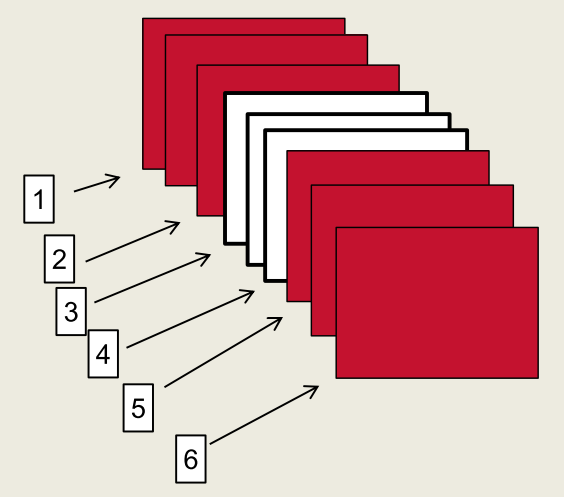
\includegraphics[width=0.4\textwidth]{eventos.png}
%	\caption{\small Ejemplo de una secuencia de eventos. Los cuadros coloreados y blancos indican eventos con poca o mucha relevancia, respectivamente. Los marcadores indican transiciones entre fases de poco y mucho interés. Obtenido de~\cite{Kelley2014}.}
%	\label{img:sleep_eventos}
%\end{figure}
%
%%Ejemplo:
%%At some location (cue), something big and orange (Tiger) moved from left to right resulting in pain (event)
%
%Además, este diseño permite que el sistema cambie su opinión sobre un evento, mediante aprendizaje reforzado. Si se repiten eventos, pero la consecuencia deja de ser la misma, entonces el sistema se acostumbra.


\subsubsection{Aspectos fuera del alcance del proyecto}\label{sec:otros_aspectos}
%% =====================================================================

A continuación se presentan algunos estudios relacionados con aspectos de una LTM que escapan de los requerimientos para este proyecto o que simplemente no son basados en la taxonomía de la memoria humana. Estos trabajos solo se presentan a modo de completitud, pues no permiten resolver el objetivo de este proyecto, sino que solo comprender otros enfoques y acercamientos a la solución. 

Thorsten et al.~\cite{Spexard2008} proponen una memoria LTM para el robot BIRON. En su trabajo, se abstraen de la clasificación entre memorias episódica y semántica, pues todos los datos de largo plazo almacenados por el robot son considerados LTM. La memoria almacena solo datos de alto nivel, obtenidos tras el procesamiento de streams de datos básicos, como cámaras, micrófonos o actuadores. Los datos almacenados corresponden a un historial de percepciones y acciones de alto nivel realizadas, como: detecciones de objetos, interacciones verbales o la descripción de movimientos realizados. A pesar de su simplicidad, esta arquitectura centralizada permite reducir las dependencias entre cada componente y el ancho de banda utilizado para retransmitir la información entre procesos.

El sistema propuesto por Ho et al.~\cite{Ho2009} busca modelar la memoria de forma suficientemente general, como para permitir el traspaso de los recuerdos de un robot a otro, independientemente de que el hardware sea distinto. El costo de esto, es que se reduce la personalización de cada robot. Por otro lado, Ho et al. además aplican la teoría \textit{Roboética}, sugerida por Veruggio y Operto~\cite{Veruggio2006}, de donde derivan restricciones de diseño, relativas al manejo de información privada de los usuarios.

La LTM procedural es estudiada por Salgado et al.~\cite{Salgado2012}, donde demuestran que a través de ella se puede mejorar el desempeño del robot en tareas repetitivas. En 2014 Winkler et al.~\cite{Winkler2014} desarrollaron CRAMm, un sistema para el manejo de memoria semántica y procedural basado en KnowRob~\cite{Tenorth2013}, con el fin de dar soporte a las tareas de manipulación de su plataforma robótica. Mediante CRAMm, el robot puede tener conocimiento de los objetos del entorno, sus posiciones habituales y las rutinas de manipulación apropiadas para cada caso. Por ejemplo, puede saber que la leche es un objeto perecible, por lo que probablemente pueda ser encontrada en el refrigerador, más aún, CRAMm provee procedimientos para abrir ese contenedor y obtener el objeto.

La LTM también ha sido implementada mediante estrategias que no siguen las estructuras de procesamiento utilizadas por la memoria humana. Por ejemplo, Kim et al.~\cite{KimMinJoo2016} plantean el uso de Deep Learning para modelar la memoria episódica y la planificación de acciones de manera holística. En su implementación, los procesos de codificación, almacenado y recuperación de episodios son manejados como uno. Así, el sistema LTM y la aplicación objetivo comparten la misma implementación, y todas las interacciones son manejadas automáticamente por la red.


%% =====================================================================

%% =====================================================================

%% =====================================================================

%% =====================================================================

%% =====================================================================

%% =====================================================================

%% =====================================================================

%% =====================================================================
%% =====================================================================
\section{Aspectos Relevantes para el Diseño}
%% =====================================================================
%% =====================================================================
%% =====================================================================

Esta sección presenta en detalle el marco teórico requerido para el diseño del sistema LTM. Se detallan aspectos de diseño para la memoria episódica y semántica. Además se revisan implementaciones de memoria emocional y relevancia histórica para modular el almacenamiento, deterioro y la adquisición de episodios.

%% =====================================================================
%% =====================================================================
%% =====================================================================
\subsection{Memoria explícita}\label{sec:ltm_exp}
%% =====================================================================
%% =====================================================================
%% =====================================================================

La implementación de un sistema de memoria episódica no puede ser completamente separada de la memoria semántica. La primera almacena eventos y su contexto espacio-temporal, a la vez que la otra almacena información sobre cada entidad del episodio. Así, es posible recordar información de un objeto y su evolución histórica ligada a los eventos almacenados.

No existe un consenso sobre los contenidos, el formato o las herramientas para implementar una memoria explícita~\cite{ltm_in_robocup}. Sin embargo, si existe una aceptación generalizada sobre los requerimientos mínimos y deseables para su diseño~\cite{Vijayakumar2014,Ho2009,Jockel2008}. Particularmente, Stachowicz en su trabajo del año 2012~\cite{Stachowicz2012} deriva un conjunto de 11 requisitos mínimos para la construcción de una memoria episódica y semántica, a partir de características cognitivas de sistemas episódicos naturales, extendidas con propiedades deseables desde un punto de vista técnico. Estos requisitos $(\mathcal{R}_{1},\ldots,\mathcal{R}_{11})$, descritos a continuación, permiten dar una base para el diseño del sistema LTM.


\subsubsection{Aspectos de diseño requeridos:}
%% =====================================================================

\begin{description}[topsep=0pt]
	\setlength\itemsep{0.2em}
	\item \RStachowicz{1} {\bfseries Contenido:}
	La información de eventos pasados debe ser recolectada e indexada respecto a su contexto espacio-temporal: Qué, dónde y cuándo pasó. El campo ``Qué'' debe permitir almacenar información variable, organizada en estructuras de datos que no se conocen de antemano y que se ajustan a diversos módulos de procesamiento. 
	
	\item \RStachowicz{2} {\bfseries Estructura:}
	Cada evento en conjunto con su contexto espacio-temporal forman una única representación integrada, que debe ser recolectada como un todo, en caso de recolectar cualquiera de las características del evento.
	
	\item \RStachowicz{3} {\bfseries Flexibilidad:}
	La información almacenada es declarativa por naturaleza, y puede ser flexiblemente almacenada. Particularmente, puede interactuar con conocimiento semántico, incluso si este fue obtenido con posterioridad a la codificación del episodio.
	
	\item \RStachowicz{4} {\bfseries Unicidad:}
	La memoria episódica cuenta con solo una instancia de cada evento para su entrenamiento, pues cada evento tiene características específicas a la situación. Es decir, cada episodio es único y no puede ser generalizado o entrenado a partir de una secuencia de episodios.
	
	\item \RStachowicz{5} {\bfseries Introspección:}
	Recuerdos episódicos pueden ser almacenados por periodos de segundos, minutos, días o años. Es posible hablar sobre eventos asociados y acceder a ellos para introspección.
	
	\item \RStachowicz{6} {\bfseries Perspectiva:}
	La memoria episódica debe lidiar con datos específicos al evento, lo que implica una perspectiva. Es decir, eventos recordados deben mantener la misma perspectiva que se tenía en la experiencia original~\cite{CLAYTON20092330}. Por otro lado, la memoria semántica generalmente se puede abstraer de la perspectiva y aspectos situacionales.
	
	\item \RStachowicz{7} {\bfseries Anidamiento:}
	Los eventos almacenados en la memoria episódica pueden variar en tiempo y extensión. Particularmente, pueden ocurrir eventos dentro del lapso temporal de otro, ambos asociados al mismo contexto episódico.
	
	\item \RStachowicz{8} {\bfseries Transposición:}
	Los eventos almacenados en la memoria episódica pueden variar en tiempo y extensión. Particularmente, un evento A puede iniciar antes B, pero terminar durante la vida de B.
	
\end{description}

\subsubsection{Aspectos de diseño deseables:}
%% =====================================================================

\begin{description}[topsep=0pt]
	\setlength\itemsep{0.2em}
	\item \RStachowicz{9} {\bfseries No intrusivo:}
	Se espera que la LTM no requiera dependencias de módulos externos para poder funcionar y representar los datos. A la vez, no puede depender en que los otros módulos no cambien la representación de sus datos.
	
	\item \RStachowicz{10} {\bfseries Eficiente:}
	El sistema debe ser lo suficientemente eficiente para tolerar el manejo de una alta tasa de eventos, sin degradar el funcionamiento del robot. Es decir, todos los eventos deben ser procesados eventualmente, aún cuando el robot esté ocupando gran parte de sus recursos, y sin generar hambruna de CPU ni de ancho de banda (de disco y red) al resto de los procesos.
	
	\item \RStachowicz{11} {\bfseries Escalable:}
	Los costos asociados al manejo de la información en la memoria (agregar, eliminar, actualizar y buscar datos) no deben exceder un límite superior, respecto a la cantidad creciente de datos almacenados. La memoria debe mantener los costos acotados, dentro de un rango que no entorpezca su uso.
	
\end{description}


%% =====================================================================
%% =====================================================================
%% =====================================================================
\subsection{Modulación de procesos cognitivos}\label{sec:theory-modulation}
%% =====================================================================
%% =====================================================================
%% =====================================================================

\todolater{Correcciones pendientes hasta implementar módulos en Bender.}

El almacenamiento, deterioro y recolección de episodios puede ser afectado por diversos factores. A continuación se detallan estudios que influencian el diseño, en cuanto a la modulación de tales procesos cognitivos, a partir de la memoria emocional y la relevancia histórica de los episodios.


\subsubsection{Memoria emocional}
%% =====================================================================
% Para más refs sobre emociones ver Deutsch2008

% uso de memoria emocional
La importancia de un evento se ve fuertemente influenciada por el estado emocional de una persona, o en este caso, el robot. Así, se puede dar prioridad a unos eventos por sobre otros, afectando los procesos cognitivos. Particularmente, un evento importante emocionalmente podría ser más fácilmente recordado, o ser almacenado por un periodo más largo~\cite{Deutsch2008}.

La implementación de la memoria emocional requiere como mínimo de un mapeo entre los estímulos percibidos por el robot y las sensaciones emocionales que estos generan. Dood et al.~\cite{Dodd2005} proponen el uso de la teoría emocional de reacciones de Haikonen~\cite{}, que considera a una emoción como una combinación de estímulos básicos. Las sensaciones elementales son: bienestar, malestar, dolor, placer e interés.
\todojocelyn{referencia a la teoría emocional de Haikonen}

Dood et al. proponen implementar las sensaciones a partir de distintos estímulos medidos en un robot:
\begin{itemize}
	\item Según las entradas de sensores. Por ejemplo, actuador que se aproxima a sus límites de movimiento físico o de fuerza, y el nivel de iluminación o ruido acústico percibido.
	\item Según el nivel de interacción con humanos. Por ejemplo, cantidad de interacciones en un periodo, ausencia de humanos o cantidad de humanos en el entorno.
	\item Según el cumplimiento de objetivos y expectativas. Por ejemplo, de acuerdo a las tareas que se lograron cumplir y los errores cometidos.
\end{itemize}

Sistemas más avanzados, incluso pueden considerar la generación de reacciones emocionales, basándose en las sensaciones derivadas anteriormente. En la Tabla~\ref{img:emotional_haikonen} se muestran las reacciones generadas según el modelo de Haikonen. Además, estas se podrían reflejar en la personalidad del robot, por ejemplo, mediante gestos, vocabulario o nivel de aceptación para realizar una acción. Kasap et al.~\cite{Kasap2010} utilizan un sistema llamado \textit{Emotion Engine}, para generar reacciones emocionales y simular cambios de personalidad de un robot, según las sensaciones percibidas.

\begin{table}[!ht]
	\centering
	\begin{tabular}{| l | l |}
		\hline
		\rowcolor{gray!50}
		Sensación Elemental & Reacción  \\ 
		\hline Bueno: gusto, aroma & Aceptación, Acercar \\ 
		\hline Malo: gusto, aroma & Rechazo, Alejar \\ 
		\hline Dolor: autoinfligido  & Alejar, Desistir \\ 
		\hline Dolor: agente externo & Agresión \\ 
		\hline Dolor: sobre esfuerzo & Sumisión \\ 
		\hline Placer & Mantener, Acercar \\ 
		\hline Acierto & Mantener atención \\ 
		\hline Desacierto & Migrar atención \\ 
		\hline Novedad & Enfocar atención \\ 
		\hline 
	\end{tabular} 
	\caption[Sensaciones elementales y reacciones en el modelo de Haikonen.]
	{\small Sensaciones elementales y sus reacciones correspondientes, según el modelo de Haikonen. Obtenido de~\cite{Dodd2005}.}
	\label{img:emotional_haikonen}
\end{table}
\todojocelyn{Sobre cita en Tabla \ref{img:emotional_haikonen}. es raro que algo propuesto por persona X salga de un paper por persona Y .. cual es la referencia original al modelo de Haikonen?}

Para su uso efectivo dentro de un esquema LTM, se espera que las sensaciones reportadas incluyan un nivel de intensidad. Según el nivel percibido en cada episodio, es posible clasificarlos entre eventos muy o poco relevantes. Los más relevantes tendrán mayor probabilidad de ser recuperados al recordar. Deutsch et al.~\cite{Deutsch2008} consideran que la intensidad de las sensaciones es importante, pues permite evitar costos de búsqueda lineales dentro de todos los episodios almacenados.

\todojocelyn{falta una frase para conectar este párrafo con lo presentado anteriormente}
En el año 1980 Plutchik~\cite{plutchik1980} presenta la Rueda de las Emociones, que se muestra en la Figura~\ref{img:plutchik}. Su trabajo es uno de los más influyentes para la clasificación de las emociones y sus respuestas. Plutchik propone 8 emociones primarias, cada una es de carácter bipolar y con un nivel de intensidad asociado: ira - miedo, alegría - tristeza, confianza - aversión, sorpresa - anticipación. La rueda además muestra 8 emociones avanzadas de carácter bipolar, formadas a partir de las 2 emociones primarias adyacentes.
\todojocelyn{y cual es la conexión de esto con tu memoria?}

\begin{figure}[!ht]
	\centering
%	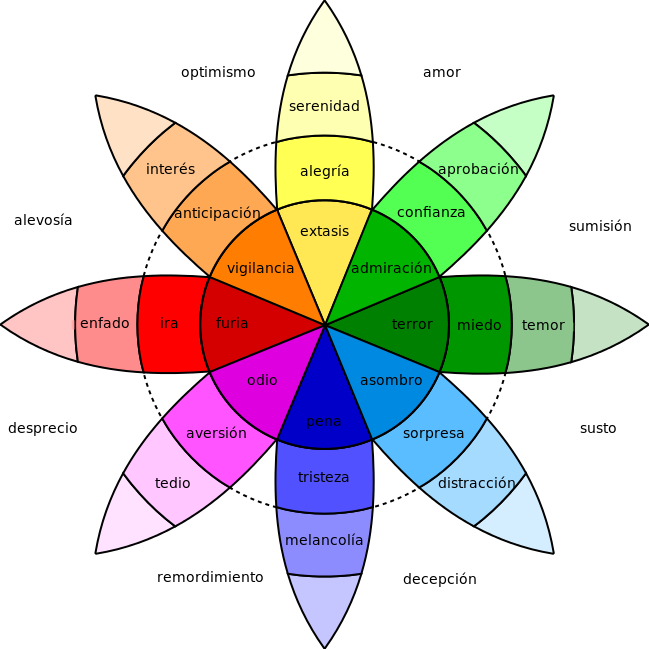
\includegraphics[width=0.7\textwidth]{plutchik-wheel.png}
\resizebox{0.75\textwidth}{!}{%
\begin{tikzpicture}[x=1.375cm,y=1.375cm]
\foreach \r in {4,3}
  \draw [dashed] circle [radius=\r];

%  {green!50!black, green!75!brown, yellow!50!white, orange, red, magenta, blue, blue!50!cyan}

\foreach \c [count=\i from 0] in  
  {gray!85!green, gray!85!brown, gray!85!yellow, gray!85!orange, gray!85!red, gray!85!magenta, gray!85!blue, gray!85!cyan}{
  \foreach \s [count=\j from 0] in {25,50,75,100}{
    \begin{scope}[rotate=\i*45]
      \clip (0,0) -- (22.5:2)
        arc (90:0:3 and 2*sin 22.5)
        arc (360:270:3 and 2*sin 22.5) -- cycle;
      \fill [fill=\c!\s!white] circle [radius=5-\j];
      \draw circle [radius=5-\j];
     \end{scope}
}}

\foreach \i in {0,...,7}
  \draw [rotate=\i*45] (0,0) -- (22.5:2)  
    arc (90:0:3 and 2*sin 22.5)
    arc (360:270:3 and 2*sin 22.5);

\foreach \emotionlist [count=\i] in
  {{terror,miedo,temor},
   {admiración,confianza,aprobación},
   {éxtasis,alegría,serenidad},
   {vigilancia,anticipación,interés},
   {furia,ira,enfado},
   {odio,aversión,tedio},
   {pena,tristeza,melancolía},
   {asombro,sorpresa,distracción}}
  \foreach \emotion [count=\j] in \emotionlist
    \node [anchor=base, font=\footnotesize, emotion label \i-\j/.try] at (\i*45-45:\j+.5) {\emotion};

\foreach \emotion [count=\i] in
{sumisión, amor, optimismo, alevosía,desprecio,remordimiento,decepción,susto}
  \node [anchor=base, font=\footnotesize]
    at (\i*45-22.5:4.75) {\emotion};

\end{tikzpicture}
}

	\caption[Rueda de las Emociones de Plutchik.]
	{\small Rueda de las Emociones de Plutchik. Cada rama representa una de las 8 emociones primarias y sus 3 niveles de intensidad.}
	\label{img:plutchik}
\end{figure}


\todojocelyn{no es posible integrar las secciones 2.4.2.1 y 2.4.2.2? dado que sigues hablando del trabajo de Dood ..}

\subsubsection{Relevancia histórica}
%% =====================================================================
% - Sobre concepto de relevancia historica
% - mezlcla y relevancia generalizada
% - algoritmo y graph
La relevancia histórica es un indicador que representa el olvido o pérdida de interés sobre un episodio en la memoria. Está directamente relacionado a la edad de un episodio, a menor antigüedad, mayor es su importancia, lo que se traduce en una mayor probabilidad de recordar ese episodio.

La implementación de relevancia histórica es estudiada por Dood et al., donde presenta una estrategia para su implementación y su interacción con la memoria emocional~\cite{Dodd2005}. Propone el uso de un indicador de relevancia generalizado, obtenido al combinar la intensidad de los dos indicadores. Además, propone un modelamiento matemático para representar el decaimiento de la relevancia histórica en el tiempo.

%\todounsure{Es necesario poner ecuaciones y curvas de decaimiento??}


\chapter{Aspectos Técnicos}\label{chapter:technical}

En este capítulo se describen los aspectos técnicos necesarios para comprender el diseño e implementación del proyecto. Primero, se presentan los componentes de software y hardware utilizados. Luego, se revisan algoritmos y conceptos computacionales utilizados en el trabajo.

%% =============================================================================

%% =============================================================================

%% =============================================================================

%% =============================================================================

%% =============================================================================

%% =============================================================================
%% =============================================================================
%% =============================================================================
\section{Componentes de software y hardware}
%% =============================================================================
%% =============================================================================
%% =============================================================================

A continuación se describen los componentes de software y hardware utilizados para el diseño e implementación del proyecto: Se hace una revisión breve de la base de datos MongoDB. Se revisan los conceptos utilizados sobre el framework robótico ROS. Se describe la librería SMACH, utilizada para la creación de máquinas de estado. Y finalmente, se presenta a Bender junto a los aspectos requeridos de su sistema operativo.

%% =============================================================================
%% =============================================================================
%% =============================================================================
\subsection{ROS}
%% =============================================================================
%% =============================================================================
%% =============================================================================

ROS \cite{ROS:2009}, acrónimo para Robot Operating System, es un proyecto que funciona como \textit{middleware} para aplicaciones robóticas, y permite resolver el problema de la comunicación entre procesos. Es una colección de herramientas, librerías y convenciones que buscan simplificar la tarea de crear comportamientos robóticos complejos y robustos, sin importar la plataforma robótica.

Fue originalmente creado por la organización WillowGarage en el 2008, y es mantenido actualmente por la Open Source Robotics Foundation (OSRF). Existe un ecosistema ROS, mantenido por la comunidad, y con cientos de módulos de software con soluciones a problemas específicos, los que pueden interconectarse para construir comportamientos más complejos. Por lo anterior, su uso se ha convertido en una práctica mundial, siendo adoptado incluso en soluciones industriales.

\subsubsection{Intraestructura}
%% =============================================================================

\paragraph{Nodo}
Es un programa ejecutable en ROS, enfocado en una tarea específica. Cada nodo puede establecer comunicación con otros a través de una interfaz ROS de tópicos o servicios.

\paragraph{Paquete}
Corresponde a un conjunto de nodos, junto a todos sus archivos necesarios para su compilación y ejecución. Cada paquete tiene asociado un nombre único en el sistema, junto a una lista de dependencias de otros paquetes. ROS provee conjunto estándar de paquetes y librerías enfocados en diversos aspectos de la robótica, que en conjunto a los paquetes mantenidos por la comunidad, permiten simplificar la construcción y mantenimiento de un robot.

\paragraph{Distribuciones} 
Una distribución es un conjunto versionado de paquetes ROS. Su propósito es permitir que los desarrolladores trabajen en un conjunto relativamente estable de dependencias, hasta que puedan avanzar a la siguiente versión. Se libera una distribución anualmente, enfocada a una versión  LTS\footnote{LTS es un acrónimo para Long-Term-Support. Una versión LTS de un software indica que éste contará con soporte a largo plazo, es decir, durante un periodo mayor a su periodo normal de vigencia.} de Ubuntu, y las versiones pares de ROS también se consideran LTS y mantienen soporte por 5 años.

\paragraph{Lenguajes de programación} ROS provee librerías oficiales para escribir nodos en los lenguajes C++ (\texttt{roscpp}\footnote{Documentación oficial de \texttt{roscpp}: \url{http://wiki.ros.org/roscpp}.}), Python (\texttt{rospy}\footnote{Documentación oficial de \texttt{rospy}: \url{http://wiki.ros.org/rospy}.}) y Common Lisp (\texttt{roslisp}\footnote{Documentación oficial de \texttt{roslisp}: \url{http://wiki.ros.org/roslisp}.}), junto a librerías experimentales para otros lenguajes.

\subsubsection{Comunicación}
%% =============================================================================

\paragraph{ROS master} Es el servidor central de ROS y provee servicios de registro al resto de los nodos. Mantiene una lista de los tópicos, servicios y parámetros disponibles, que han registrado los nodos activos. Su principal funcionalidad es permitir que cada nodo pueda encontrar a los otros. Una vez establecida la comunicación, los nodos se comunican en una red P2P\footnote{En una red P2P (peer-to-peer) los participantes se comunican total o parcialmente sin requerir un servidor intermediario.}. Comúnmente la comunicación en ROS se realiza mediante el protocolo HTTP, bajo un transporte TCP, sin embargo, los nodos pueden ser configurados para utilizar un transporte basado en UDP. Por lo tanto, ROS permite el manejo de nodos de manera distribuida, siempre que cada máquina tenga acceso a la red del computador ejecutando el ROS master.

\paragraph{Mensaje} Es una estructura de datos utilizada para comunicar un nodo con otro. Se definen en un mensaje de tipo \texttt{.msg}, a partir de tipos de dato básicos en ROS y otros mensajes. Durante la compilación se genera el código para poder utilizarlos mediante las librerías ROS de cada lenguaje de programación disponible.

\paragraph{Tópico} Permite que los nodos de comuniquen a través de mensajes, y está basado en el patrón de diseño observador. Cada tópico es un canal de comunicación que transmite mensajes ROS de un tipo predefinido. Cada nodo puede publicar simultáneamente en uno o más tópicos. Cada nodo puede suscribirse a los tópicos que desee, siendo notificado por cada mensaje entrante. Esto se describe en el diagrama de la Figura \ref{img:ros-topic}.

\begin{figure}[!h]
	\centering
	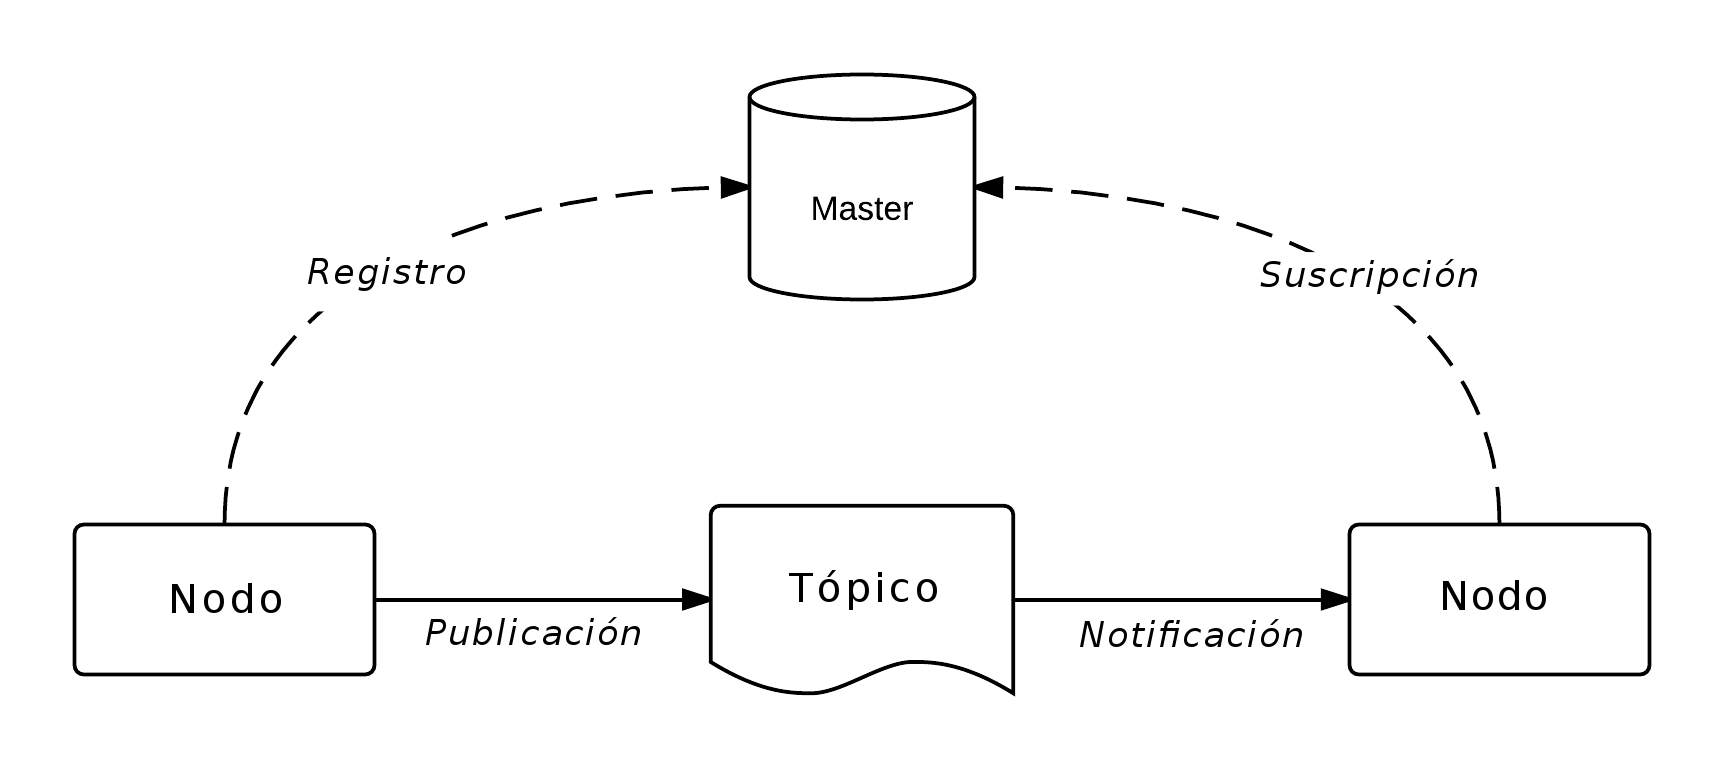
\includegraphics[width=0.8\textwidth]{ROS-master-node-topic-esp.png}
	\caption{\small Diagrama de la comunicación mediante tópicos en ROS. El ROS master se encarga de establecer el proceso de comunicación entre los nodos involucrados. Luego los nodos se comunican {\bfseries unidireccionalmente} usando el tópico establecido.}
	\label{img:ros-topic}
\end{figure}

\paragraph{Servicios} Es una forma de comunicación cliente-servidor de carácter síncrono. Se construyen a partir de una estructura de datos de tipo \texttt{.srv}, que especifica mensajes ROS de petición y respuesta, disponible tras la compilación. Cada nodo (servidor) puede proveer uno o más servicios. Cada nodo (cliente) puede enviar peticiones al servidor. Las peticiones son de carácter bloqueante, hasta que una respuesta desde el servidor sea recibida.

\paragraph{Acciones} Esta forma de comunicación se construye a partir de tópicos y servicios, mediante la librería \texttt{actionlib} \footnote{Documentación oficial de \texttt{actionlib}: \url{http://wiki.ros.org/actionlib}.}. Está enfocada en la resolución de tareas de largo plazo, y funciona a través de metas solicitadas por el cliente. El servidor mantiene una máquina de estados que recibe peticiones (servicio) e informa constantemente sobre el estado del proceso y su resultado (tópicos). La estructura de datos utilizada es de tipo \texttt{.action}, que especifica mensajes ROS para la petición, el \textit{feedback} y el resultado.

\paragraph{Servidor de parámetros} ROS provee un servidor para almacenar, modificar y obtener parámetros compartidos entre los nodos. Éstos permiten la configuración del programa sin tener que recompilar el código, y funcionan como el estándar para el manejo de parámetros. La configuración por defecto puede ser especificada en archivos usando el formato YAML.


\subsubsection{Herramientas}
%% =============================================================================

\paragraph{Pluginlib} Es un paquete oficial de ROS\footnote{Documentación oficial de \texttt{pluginlib}: \url{http://wiki.ros.org/pluginlib}.} que provee herramientas para escribir y cargar plugins dinámicamente en nodos C++. La librería permite delegar la implementación de funcionalidades específicas a los usuarios. El nodo que ocupará el plugin debe definir una clase abstracta a ser implementada. Mientras que los paquetes proveedores deben registrar las librerías con sus implementaciones, para que los plugins queden disponibles en el sistema.

\paragraph{Roslaunch} La librería \texttt{roslaunch}\footnote{Documentación oficial de \texttt{roslaunch}: \url{http://wiki.ros.org/roslaunch}.} es una herramienta que permite la ejecución y configuración de múltiples nodos, a través de sólo un comando en la consola del sistema. Utiliza archivos en formato XML y con extensión \texttt{.launch}, donde se define un árbol de nodos y otros archivos \textit{launch} a ser ejecutados. Esta herramienta permite modularizar la ejecución de un sistema robótico complejo, compuesto generalmente por decenas de nodos.

%\paragraph{Rviz}
%\paragraph{Rosbag} (probablemente se ocupará para test suite)


%% =============================================================================
%% =============================================================================
%% =============================================================================
\subsection{MongoDB}\label{sec:mongodb}
%% =============================================================================
%% =============================================================================
%% =============================================================================

\subsubsection{Conceptos:}

MongoDB es una base de datos no relacional orientada a documentos tipo JSON, donde los campos pueden variar de documento a documento y la estructura de datos puede ser modificada en el tiempo \cite{MongoDB}. MongoDB está diseñada para funcionar de manera distribuida, proveer alta disponibilidad, escalamiento horizontal y distribución geográfica. Es una base de datos gratis y de código libre, publicada bajo la licencia GNU AGPL.

MongoDB representa documentos JSON en un formato binario denominado BSON. BSON extiende JSON a través de nuevos tipos de datos, introduce campos ordenados y está diseñado para proveer eficiencia al codificar y decodificar la información en distintos lenguajes. 

Los documentos son organizados en \textit{colecciones}, cada una destinada a almacenar información asociada a un concepto particular. MongoDB provee funcionalidades para consultas, indexado y realizar agregaciones de los datos almacenados.

MongoDB provee drivers para diversos lenguajes de programación, entre ellos C++, Java y Python. Para este proyecto, el driver de interés es el de C++11\footnote{Documentación del driver de MongoDB para C++:  \url{http://mongodb.github.io/mongo-cxx-driver/}.}.

En su configuración por defecto, el servidor de MongoDB soporta documentos de hasta 16MB de tamaño, lo que restringe la información a almacenar, pero permite mantener acotados los costos de las operaciones sobre la base de datos. Este límite puede ser removido al modificar el algoritmo de almacenamiento a GridFS, que divide documentos grandes en subdocumentos menores a 16MB, para ser tratados normalmente.

\subsubsection{Interfaz ROS:}

MongoDB es una de las dependencias de \textit{MoveIt!}\footnote{Documentación oficial de MoveIt!: \url{https://moveit.ros.org/}.}, librería estándar utilizada para la manipulación de objetos, de uso extendido en la comunidad robótica. Por lo tanto, MongoDB ya está instalada y funcionando en muchos robots de servicio basados en ROS. 

El equipo desarrollador de MoveIt! y sus paquetes ROS relacionados mantiene el paquete \texttt{warehouse\_ros\_mongo}\footnote{El paquete ROS \texttt{warehouse\_ros\_mongo} está disponible en: \url{https://github.com/ros-planning/warehouse\_ros\_mongo}.}, que provee una interfaz ROS al driver en C++ para MongoDB. MoveIt! y sus dependencias son consideradas estables, al menos durante el periodo de la última distribución ROS, con fecha de caducidad para el 2023.

\texttt{warehouse\_ros\_mongo} permite definir colecciones destinadas a almacenar mensajes ROS, de manera binaria. Cada documento es construido a partir del mensaje ROS serializado (mediante su API ROS), sumado a un conjunto de metadatos utilizados para la definición de índices y consultas. Actualmente, la API sólo soporta la definición de metadatos de los tipos \texttt{bool}, \texttt{int}, \texttt{double} y \texttt{std::string} en C++.


%% =============================================================================
%% =============================================================================
%% =============================================================================
\subsection{SMACH}
%% =============================================================================
%% =============================================================================
%% =============================================================================

SMACH es una librería en Python para la creación y ejecución de máquinas de estado. Permite crear rápidamente comportamientos robóticos complejos, basados en capacidades de alto nivel de un robot. Está diseñada para ser independiente de ROS, pero provee una interfaz para su uso. Se puede encontrar en el conjunto de paquetes ROS denominado \texttt{executive\_smach}\footnote{Documentación oficial de SMACH disponible en: \url{http://wiki.ros.org/smach}.}.

\begin{figure}[!h]
	\centering
	\includegraphics[width=0.8\textwidth]{smach-sample.png}
	\caption{\small Ejemplo de máquina de estado construida en SMACH para la representación de una rutina de carga automática de baterías. Obtenido desde la documentación oficial.}
	\label{img:SMACH-sample}
	\todounsure{Es necesario poner la figura en español??}
\end{figure}



En SMACH una maquina de estado está compuesta por un conjunto de estados y sus transiciones. La librería soporta anidamiento, por lo que cualquier estado puede ser reemplazado por otra máquina de estado disponible. Cada estado debe proveer una función \texttt{execute} a ser ejecutada cuando esté activo. En la Figura \ref{img:SMACH-sample} se presenta un ejemplo de un comportamiento robótico complejo implementado en SMACH, que representa el proceso de recarga de baterías en un robot. Según las condiciones encontradas se activarán distintas transiciones, pero en el caso básico la rutina es la siguiente: El robot navega a la estación de carga, se posiciona, manipula el conector, se conecta y espera.

%% =============================================================================
%% =============================================================================
%% =============================================================================
\subsection{UChile ROS Framework}\label{sec:URF}
%% =============================================================================
%% =============================================================================
%% =============================================================================

\subsubsection{Conceptos}

UChile ROS Framework (URF) hace referencia al sistema de software desarrollado en el laboratorio de robótica del Departamento de Ingeniería Eléctrica de la Universidad de Chile, para sus robots de servicio. El sistema cuenta con 10 años de desarrollo y está orientado a cumplir los requisitos de la competencia RoboCup en su categoría @Home.

URF está construido sobre ROS y en una estructura de 4 capas:
\begin{enumerate}
\item La primera capa contiene todas las dependencias del sistema, ya sean de ROS o no. Es la única capa que contiene sólo código externo.
\item  Sobre la primera capa se monta una capa ROS de bajo nivel, con herramientas y librerías comunes, sumado a los drivers necesarios para manejar cada robot (módulos de \textit{Hardware} en la Figura \ref{img:URF}).
\item La capa intermedia alberga capacidades robóticas avanzadas, relacionadas a percepción robótica, manipulación de objetos, navegación autónoma e interacción Humano-Robot (sección \textit{Módulos ROS} del diagrama).
\item La última capa \textit{de alto nivel} es desarrollada en Python, con interfaces para el uso de las capacidades de menor nivel, y es utilizada para la elaboración de maquinas de estado y comportamientos robóticos complejos mediante SMACH (cuadros \textit{Interfaz ROS-python} y \textit{State Machine} del diagrama).
\end{enumerate}

\begin{figure}[!h]
	\centering
	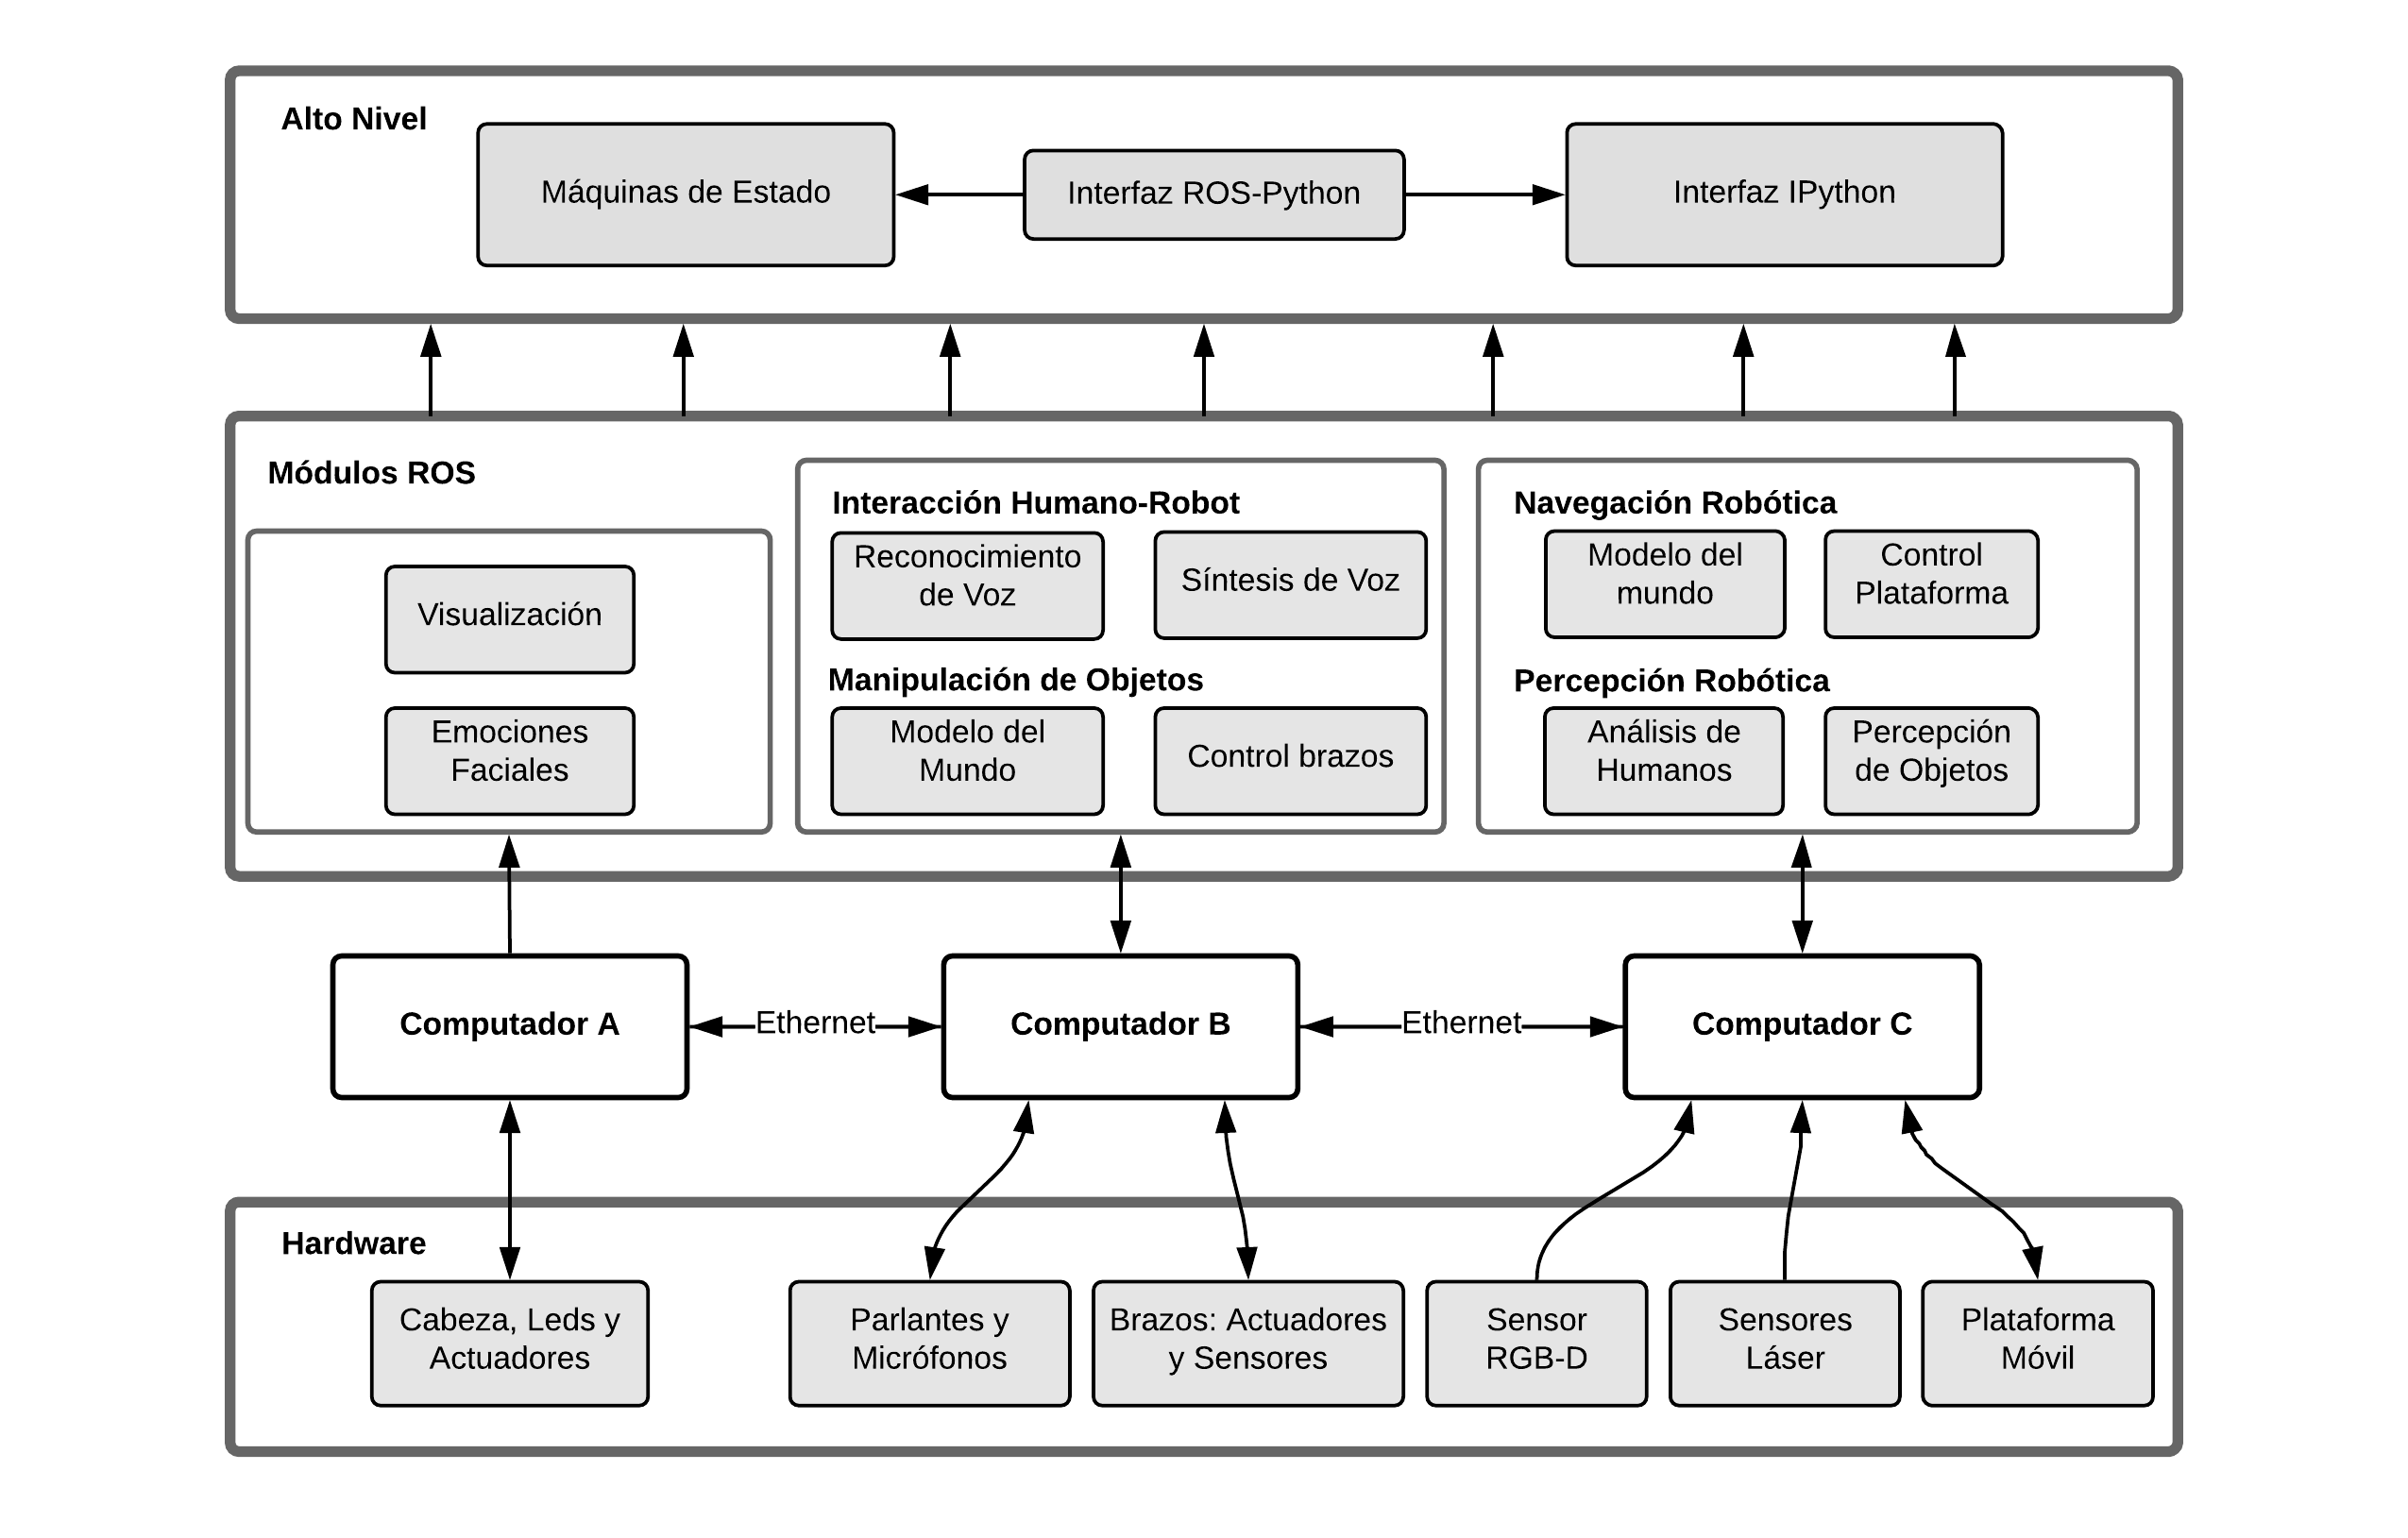
\includegraphics[width=0.8\textwidth]{URF-esp.png}
	\caption{\small Diagrama de UChile ROS Framework utilizado en el robot Bender.}
	\label{img:URF}
\end{figure}

Todos los módulos de URF son de código libre, a excepción de los algoritmos relacionados con percepción y la interfaz de alto nivel. El código se almacena públicamente en la organización \textit{uchile-robotics} en GitHub\footnote{Organización \textit{uchile-robotics} y URF en GitHub: \url{https://github.com/uchile-robotics}}.


\subsubsection{Memoria a corto y largo plazo}
%% =============================================================================

En un robot implementado sobre URF es posible acceder a la información compartida por sus procesos. Cualquier módulo ROS en el sistema tiene acceso a los datos extraídos desde sensores y luego generados en post-procesamientos, junto al acceso para controlar el hardware.

Existen algunas formas de memoria implementadas en URF, comparables a los conceptos definidos para la memoria humana. También se pueden dividir en de corto y largo plazo:

Como STM, se puede definir como memoria de trabajo a todo el flujo de información presente durante la ejecución del robot. Lo que incluye datos sensados, procesamientos y acciones realizadas. Generalmente tales datos no son almacenados para posteriores ejecuciones.

A manera de LTM, se puede encontrar una memoria procedural, relacionada con todo el conocimiento almacenado que posee el robot para cumplir ciertas tareas. Caen en esta categoría: modelos para percepción robótica, modelos para reconocimiento de voz y patrones, bases de datos de movimientos precalculados para manipular objetos y acciones predefinidas que se utilizan para controlar el robot.

También se pueden encontrar especializaciones de memoria LTM semántica. Ejemplos de esto son: El mapa que se conoce del entorno, junto a los lugares y objetos anotados en él. Diccionarios con información anotada sobre entidades y sus características, cómo personas y objetos. Bases de datos con imágenes anotadas para el reconocimiento de objetos y personas. 

Sin embargo, en URF no existen formas de memoria emocional ni episódica de largo plazo. Luego, toda interacción realizada por los robots está limitada a la información obtenida desde el inicio al término de cada rutina.


%% =============================================================================
%% =============================================================================
%% =============================================================================
\subsection{Bender}
%% =============================================================================
%% =============================================================================
%% =============================================================================
%% -----------------------------------------------------------------------------

Bender es un robot humanoide creado el año 2007 en el laboratorio de robótica del Departamento de Ingeniería Eléctrica de la Universidad de Chile. El equipo UChile Homebreakers es el encargado de su desarrollo y  su objetivo es ser un mayordomo para el hogar, funcionando de manera autónoma para apoyar en tales labores \cite{uchile-robotics}.

En cuanto a actuadores, el robot cuenta con 2 brazos antropomórficos de 6 grados de libertad cada uno, una base móvil diferencial Pioneer 3-AT, un cuello que permite rotaciones en dos ejes cartesianos; pudiendo imitar gestos de asentimiento y negación, y finalmente, una cabeza que puede mostrar expresiones faciales mediante movimientos de su boca, orejas, cejas y cambios de colores alrededor de los ojos.

El robot cuenta con los siguientes sensores: un laser Hokuyo UTM-30LX, un laser Hokuyo URG-04LX-UG01, un micrófono M-Audio Producer USB y una cámara de profundidad ASUS Xtion Pro.

El software de Bender está basado en el framework URF. Su arquitectura de software utiliza  ROS para el manejo de componentes de bajo y medio nivel. La capa de alto nivel, escrita en python, se abstrae de ROS y permite la creación de comportamientos complejos mediante máquinas de estado. Todos los módulos que interactúan con sensores y actuadores están implementados en ROS.

\begin{figure}[!h]
	\centering
	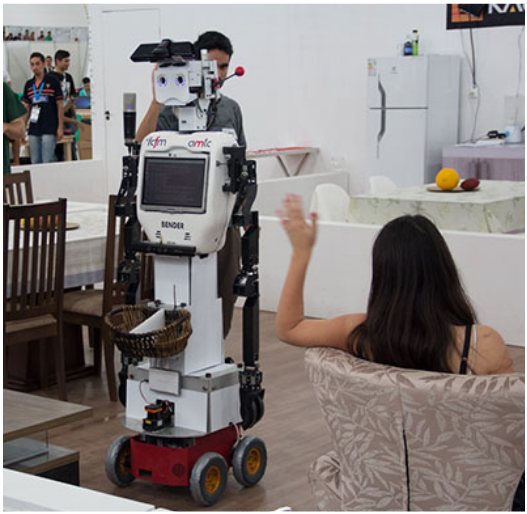
\includegraphics[width=0.4\textwidth]{bender.png}
	\caption{\small Robot Bender en competencia RoboCup@Home 2015.}
	\label{img:bender}
\end{figure}

\todoimprove{Sobre la cantidad de paquetes ROS, nodos, tópicos y mensajes disponibles.}
\todoimprove{API a ocupar para acceder a datos del robot.}


%% =============================================================================

%% =============================================================================

%% =============================================================================

%% =============================================================================

%% =============================================================================

%% =============================================================================

%% =============================================================================
%% =============================================================================
%% =============================================================================
\section{Algoritmos y conceptos computacionales}
%% =============================================================================
%% =============================================================================
%% =============================================================================
\todounsure{TODA ESTA SECCIÓN PODRÍA SER ELIMINADA....????}
\todounsure{convex hull}
\todounsure{procesamiento de imágenes: degradación de streams}
\todounsure{Algs utilizados para emociones implementadas en robot}
\todounsure{Sistemas de coordenadas?? Frames?}




\chapter{Diseño}\label{chapter:diseno}

En este capítulo se revisa el diseño del sistema LTM implementado en el trabajo. El capítulo es extenso y algunos puntos son muy detallados, por lo que se inicia con una revisión general del sistema LTM diseñado, con el fin de guiar su exposición. Considerando esto, se describe el diseño del trabajo, iniciando desde sus requerimientos hasta su integración al robot. Primero se presentan todos los requerimientos de diseño y se elabora un conjunto de validaciones que permitirán guiar el diseño, implementación y posterior evaluación del trabajo. En las siguientes 4 secciones se describe la arquitectura del sistema LTM: se revisa el diseño de los episodios, su estructura de datos y limitantes; se estudia el diseño del modelo de datos para la memoria episódica y su relación con los componentes semánticos; en tercer lugar, se presenta el diseño del servidor LTM; finalmente, se definen la interfaz episódica y los componentes específicos a implementar para el robot Bender.


\section{Revisión General}

A continuación se presenta una revisión general del sistema LTM diseñado, junto a algunas consideraciones relevantes para la comprensión de este.

\subsection{Conceptos}

Acá se presentan algunas revisiones sobre conceptos utilizados en el capítulo y aclaraciones sobre la terminología empleada.

\ltmconcept{Usuario versus operador}
Primero, se hará la distinción entre el usuario del sistema y el operador de este. En adelante, se utilizará el término \textit{usuario} para indicar a la(s) persona(s) encargadas de utilizar y modificar el software LTM para un robot en particular, es decir, un usuario es un \textit{desarrollador} de software. Por otro lado, los términos \textit{operador} y \textit{humano} serán utilizados para referirse a alguien que posiblemente interactuaría con el robot. Por lo general, en casos de prueba, un usuario hace el papel de operador, sin embargo, notar esta diferencia es relevante. Finalmente, se utilizará el término \textit{robot} para referirse al robot objetivo donde se implementa el sistema LTM. A modo de ejemplo, el equipo UChile Homebreakers sería un \textbf{usuario} del sistema LTM implementado en el \textbf{robot} Bender, mientras que una persona del público con quien interactúa el robot es llamada \textbf{operador}.

\ltmconcept{Memoria episódica versus semántica} Ya que ambos son términos recurrentes en este informe, merece la pena la siguiente aclaración. Un \textit{episodio} almacena la información de qué, dónde y cuándo sucedió un evento. La \textit{memoria episódica} es una colección de episodios. La \textit{memoria semántica} es una colección de información sobre \textit{entidades} particulares. La \textit{memoria LTM} se compone de las memorias episódica y semántica, relacionadas por el qué sucedió, respecto a las entidades conocidas.

\ltmconcept{Tareas y comportamientos} Una \textit{tarea} hace referencia a toda actividad realizada por el robot durante su funcionamiento normal, para cumplir con sus obligaciones como robot doméstico. Ejemplos de esto son la interacción con humanos y el aseo del hogar. En adelante, se utilizarán los términos de \textit{tarea} y \textit{comportamiento} para indicar este concepto.

\subsection{Sistema LTM} 

Según se detalla en las siguientes secciones del capítulo, el sistema LTM diseñado emula una memoria LTM humana con componentes episódicos, semánticos y emocionales. A modo general, en el diagrama de la Figura \ref{img:diagrama-ltm-simple} se presenta el funcionamiento del sistema LTM diseñado. En primer lugar, se recopila información a partir de las tareas que realiza el robot y su memoria de trabajo, para generar los episodios a almacenar. Luego, el sistema se encarga de mantener los datos y responder las consultas episódicas o semánticas que se requieran.

\begin{figure}[!ht]
	\centering
	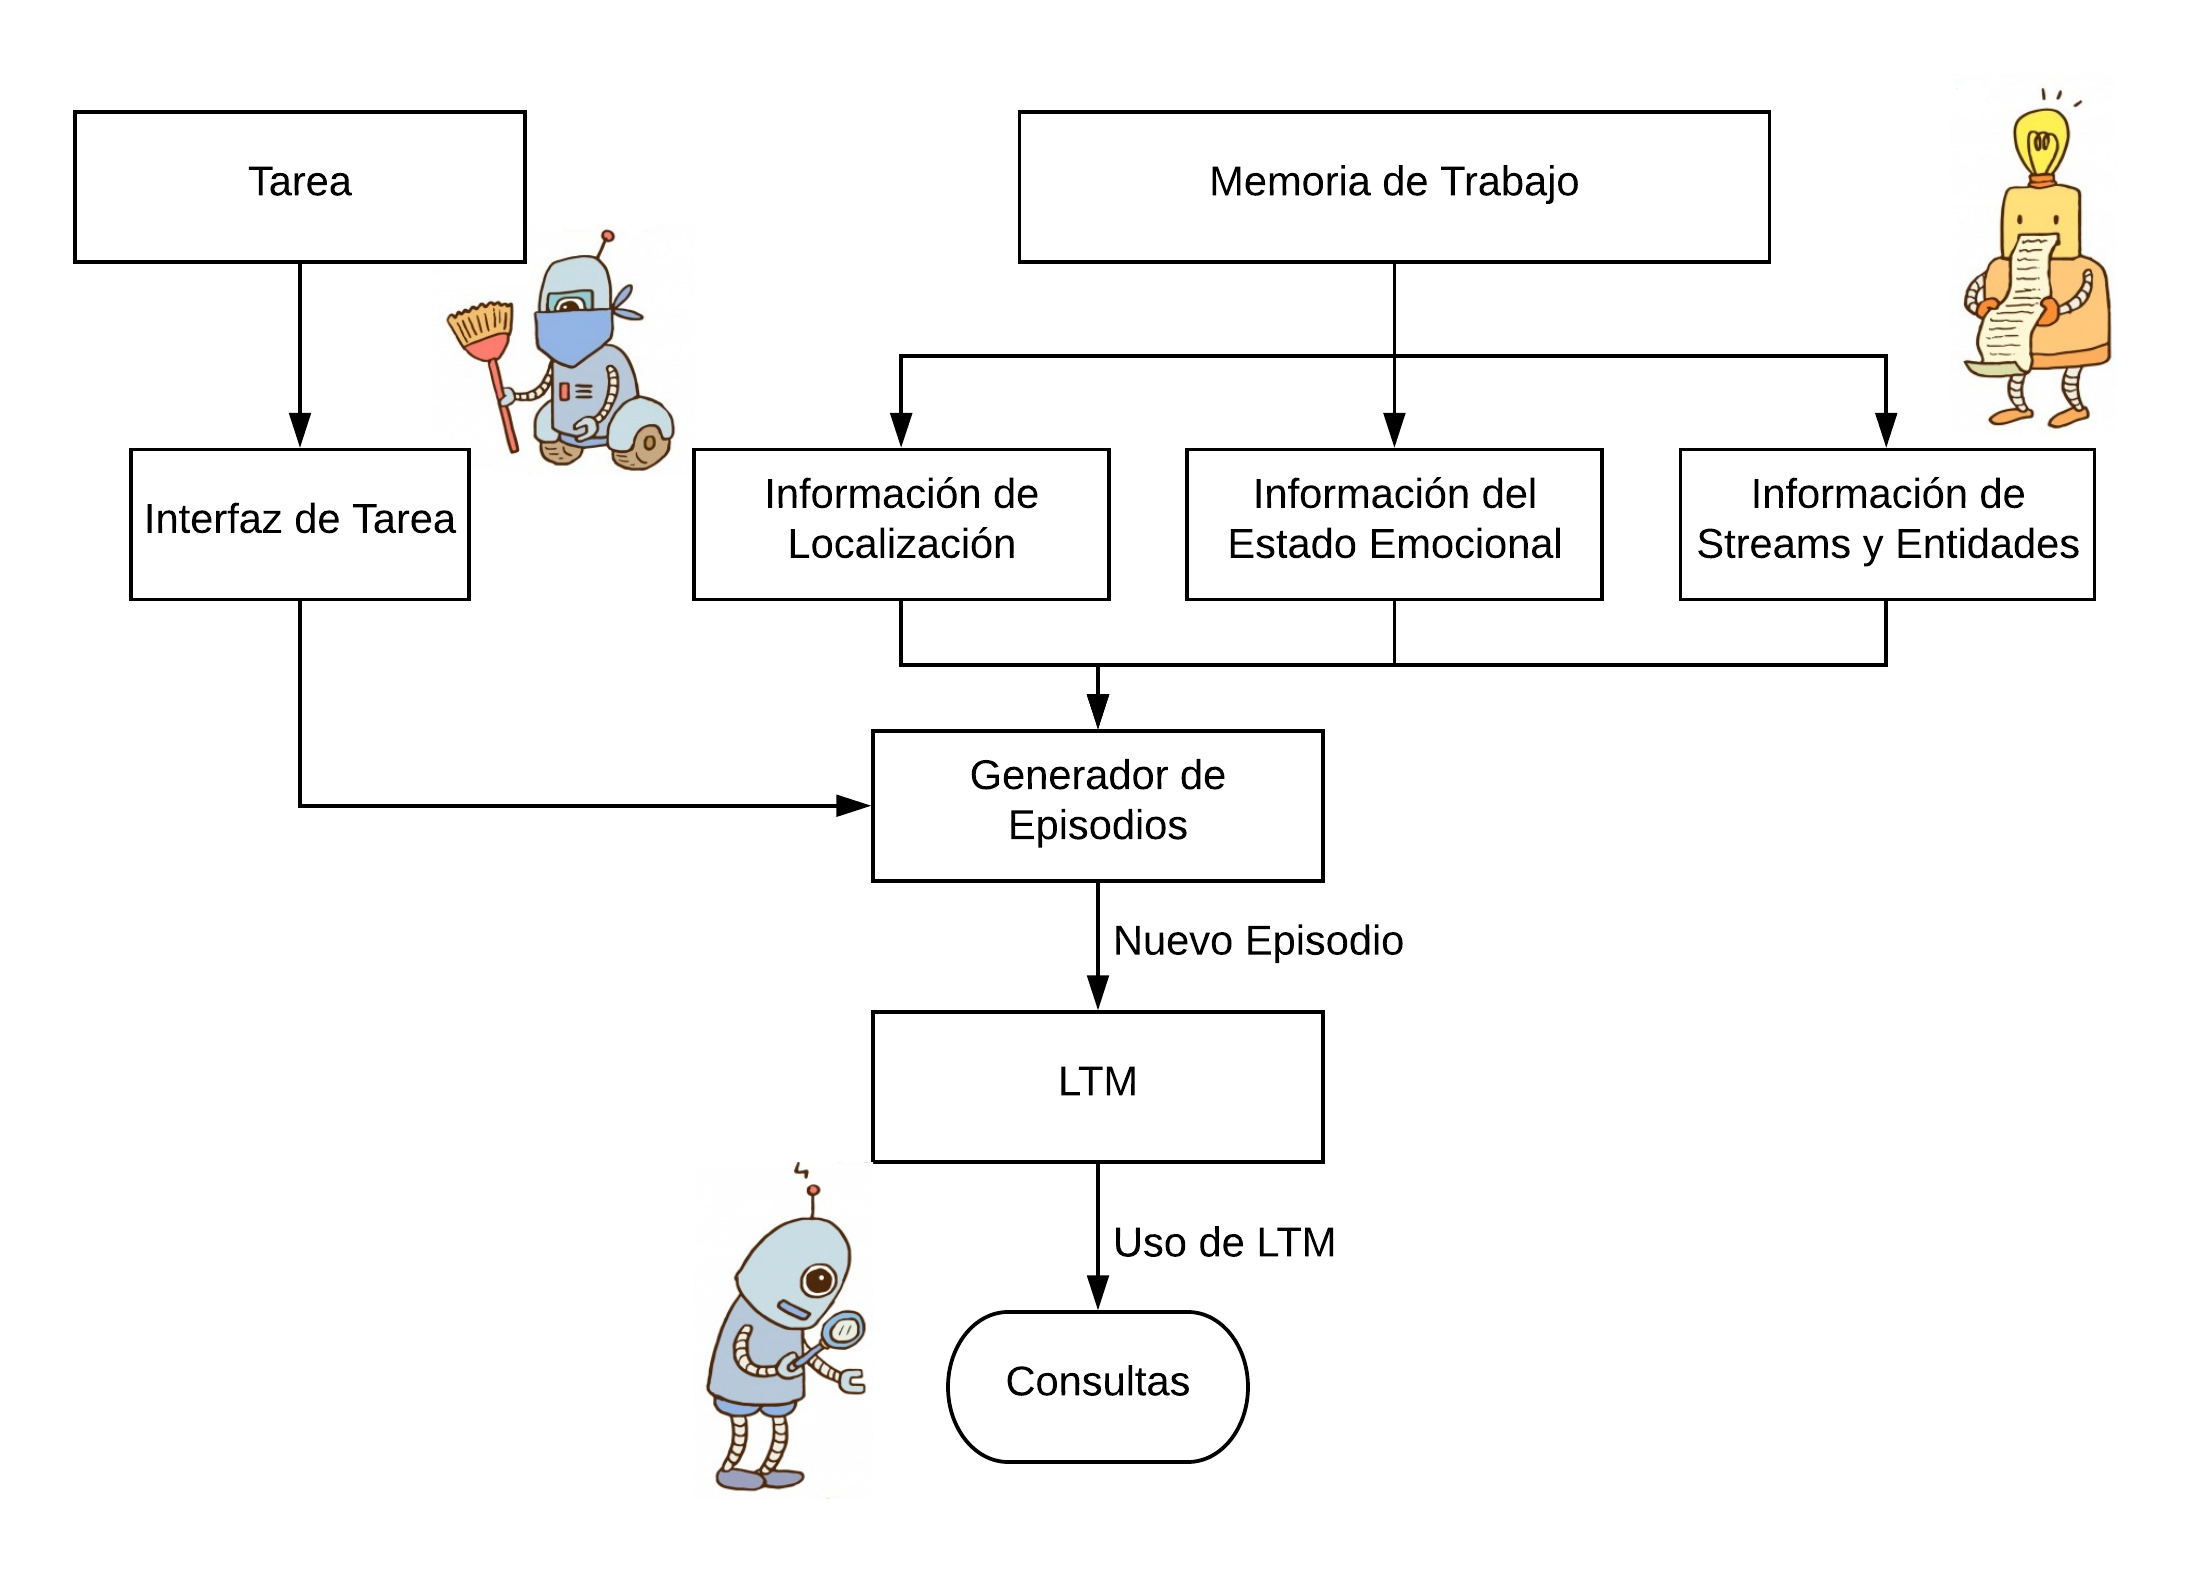
\includegraphics[width=\textwidth]{ltm-simple.png}
	\caption[Diagrama funcional del sistema LTM diseñado.]
	{\small Diagrama general del sistema LTM diseñado. Los episodios son generados a partir de información extraída sobre la tarea que ejecuta el robot y su memoria de trabajo disponible en el momento. La información almacenada puede ser consultada posteriormente.}
	\label{img:diagrama-ltm-simple}
\end{figure}

\ltmconcept{Tarea} Las tareas realizadas por el robot son utilizadas para indicar el inicio y término de un episodio y conocer la actividad realizada por el robot. Una tarea puede ser dividida en diversas subtareas más detalladas. La interfaz de tarea es utilizada para acceder a la información anterior e iniciar la generación de nuevos episodios.

\ltmconcept{Memoria de trabajo}
Cada episodio generado debe poder responder a las consultas dónde y qué sucedió, para lo que se recopila información de localización y de las entidades de interés. Además, la información del estado emocional del robot permite asignar una relevancia a los episodios almacenados.  Todos los datos anteriores son recopilados a partir de la memoria de trabajo del robot, durante la ocurrencia del episodio.

\ltmconcept{Generador de episodios}
La generación de episodios utiliza la interfaz de tarea para reconocer nuevos episodios, y la memoria de trabajo del robot, para recopilar los datos necesarios para crear el episodio. Un episodio es generado por cada tarea y subtarea registrada.

\ltmconcept{Servidor LTM}
El servidor LTM hace referencia al programa encargado de almacenar, mantener y proveer interfaces de consulta para la memoria a largo plazo generada. El servidor utiliza la base de datos MongoDB para almacenar las memorias episódica y semántica. Es diseñado para funcionar en ROS y proveer una API de registro y consulta de episodios.

\ltmconcept{Consultas}
A través de la API de consulta del servidor LTM, es posible adquirir información episódica y semántica. Las consultas se construyen utilizando el lenguaje de consultas que provee MongoDB en formato JSON. El sistema es capaz de responder consultas como: qué sucedió en cierta fecha o hablar sobre una persona en particular, sus datos y cómo se ha modificado su conocimiento sobre ella en el tiempo.

\ltmconcept{Generalidad y sistema de plugins}
El sistema LTM está diseñado para ser utilizado en Bender y otros robots, mediante el uso de un sistema de plugins. Ya que la información semántica a almacenar depende del robot objetivo, el sistema permite la definición de sus contenidos mediante cualquier estructura de datos representable en un mensaje ROS. Luego, la interfaz de tarea y las interfaces para acceder a la memoria de trabajo deben ser implementadas por el usuario, mediante una serie de plugins adecuados al robot.  Particularmente, el sistema LTM requiere la implementación de 4 plugins, para recopilar información sobre la ubicación del robot, emociones del robot, streams de datos percibidos y entidades.

\ltmconcept{Integración en Bender}
Para el caso de Bender, este trabajo provee implementaciones de cada uno de los plugins requeridos. Por un lado, las tareas son recopiladas desde máquinas de estado en SMACH. Por otro lado, se implementan plugins para acceder al sistema de localización del robot, recopilar información emocional y para recopilar datos sobre las entidades modificadas durante la tarea.




%% =============================================================================
%% =============================================================================

%% =============================================================================
%% =============================================================================

%% =============================================================================
%% =============================================================================

%% =============================================================================
%% =============================================================================
\section{Requerimientos y Validaciones}
%% =============================================================================
%% =============================================================================
%% =============================================================================

A continuación se presentan los requisitos de diseño sobre los que se construye el trabajo y las validaciones generadas a partir de ellos. Primero, se da una descripción breve sobre el origen y razón de los requisitos. Luego, se presenta un listado formal de todos los requerimientos, escritos de una forma clara y verificable. Para concluir, se presenta un conjunto de pruebas que busca validar cada requerimiento expuesto.

%% =============================================================================
%% =============================================================================
%% ============================================================================= 
\subsection{Objetivos del sistema}
%% =============================================================================
%% =============================================================================
%% =============================================================================

El primer conjunto de requisitos se deriva a partir de los objetivos del trabajo y sus alcances, presentados en la Sección~\ref{sec:objetivos}. En adelante se referirá a estos como \textit{requisitos de proyecto}.
\begin{description}
\item \RPlabelDef{1} Diseño de LTM episódica y semántica para robots de servicio domésticos, debe basarse en los 11 requerimientos para una memoria episódica planteados por Stachowicz~\cite{Stachowicz2012} y presentados en la Sección~\ref{sec:ltm_exp}.
\item \RPlabelDef{2} Este diseño debe considerar la modulación de los procesos cognitivos mediante memoria emocional.
\item \RPlabelDef{3} El diseño del sistema debe soportar el concepto de relevancia histórica.
\item \RPlabelDef{4} Además, los episodios deben manejar un indicador de relevancia generalizada, que encapsule todos los demás indicadores en solo uno.
\item \RPlabelDef{5} Diseño del sistema debe ser agnóstico del robot a utilizar.
\item \RPlabelDef{6} El trabajo debe ser integrado en Bender.
\end{description}


%% =============================================================================
%% =============================================================================
%% =============================================================================
\subsection{Requerimientos de sistema}
%% =============================================================================
%% =============================================================================
%% =============================================================================

Se desarrolló un documento con 26 requisitos de sistema, derivados a partir de los objetivos revisados en la sección anterior. Para evitar extender innecesariamente este informe, el documento desarrollado es de carácter semiformal, es decir, por cada requisito de sistema solo se presenta: su descripción, su numeración y el requisito de proyecto asociado. En adelante, cada requisito será indicado por su prefijo y numeración de la forma \RSlabel{XX}. El listado de requisitos es extenso y puede ser encontrado en el Anexo~\ref{appendix:req-sistema} junto con la matriz de trazabilidad entre requisitos de proyecto y sistema.

Los requisitos se pueden separar en 4 categorías de acuerdo a su finalidad:
\begin{enumerate}
\item \RSlabel{01}: Requisito sobre diseño agnóstico del robot objetivo. Ver \RPlabel{5}.
\item \RSlabel{02}-\RSlabel{18}: Requisitos derivados de reglas episódicas de Stachowicz. Ver \RPlabel{1}.
\item \RSlabel{19}-\RSlabel{22}: Requisitos sobre relevancias episódicas. Ver \RPlabel{2}, \RPlabel{3}, \RPlabel{4}.
\item \RSlabel{23}-\RSlabel{26}: Requisitos sobre la integración en Bender. Ver \RPlabel{6}.
\end{enumerate}

%% =============================================================================
%% =============================================================================
%% =============================================================================
\subsection{Validaciones}
%% =============================================================================
%% =============================================================================
%% =============================================================================

También se desarrolló un documento (semiformal) con validaciones para cada uno de los requisitos de sistema en el documento. Las validaciones sirven como guía para la implementación del trabajo y el resultado de su ejecución es presentado en el Capítulo~\ref{chapter:results}. El listado completo es extenso y se encuentra en el Anexo~\ref{appendix:validations}.

El documento consta con alrededor de 37 validaciones, separadas en 3 categorías. Cada validación se identifica por un prefijo y numeración de la forma \Vlabel{T}{XX} (V: Validación, T: Tipo, XX: numeración). Además, cada una indica su requisito de sistema asociado. Las categorías son las siguientes:
\begin{enumerate}
	\item \Vlabel{A}{XX}: Validaciones funcionales. Tienen como objetivo verificar que el sistema LTM cumple con todos los requisitos mínimos de funcionalidad, exceptuando los de integración con el robot Bender. En este caso, las validaciones pueden ser ejecutadas mediante simulaciones.
	\item \Vlabel{B}{XX}: Validaciones de integración con Bender. Tienen como objetivo verificar que el sistema LTM cumple con los requisitos de integración con el robot Bender. Para esto, se debe integrar el sistema al robot y ejecutar las pruebas en sus computadores.
	\item \Vlabel{C}{XX}: Validaciones de desempeño. Tienen como objetivo medir el desempeño del sistema LTM en términos de escalabilidad y eficiencia de este, para el caso de uso del robot Bender.
\end{enumerate}

Las validaciones \Vlabel{C}{XX} de eficiencia tienen por objetivo medir el uso de recursos en término de la tasa de operaciones que debe soportar el sistema LTM en Bender. Se construyen a partir del requisito de sistema \RSlabel{15}. Las validaciones de escalabilidad se construyen a partir del requisito de sistema \RSlabel{16}. Estas tienen por objetivo medir el costo en tiempo de las operaciones de inserción y búsqueda de episodios, en función de la cantidad de episodios almacenados en la base de datos.

En el Anexo~\ref{appendix:validations} se presenta la matriz de trazabilidad indicando la relación entre cada requisito de sistema y las validaciones asociadas.


%% =============================================================================
%% =============================================================================

%% =============================================================================
%% =============================================================================

%% =============================================================================
%% =============================================================================

%% =============================================================================
%% =============================================================================
%% =============================================================================
\section{Diseño de Episodios}\label{sec:ep_design}
%% =============================================================================
%% =============================================================================
%% =============================================================================

A continuación presentan las decisiones de diseño seguidas para la representación de los datos episódicos mediante mensajes de ROS. Se estudia el formato a utilizar para el almacenamiento de cada episodio, seguido de la estructura de datos tipo árbol que soporta sus anidamientos. Luego se explica el diseño de los campos episódicos (\textit{What, When, Where}), la representación de la memoria semántica y el manejo de relevancias episódicas. Finalmente, se introducen los metadatos asociados a cada episodio y las limitantes del diseño episódico desarrollado.


%% =============================================================================
%% =============================================================================
%% =============================================================================
\subsection{Formato y representación}
%% =============================================================================
%% =============================================================================
%% =============================================================================

% SOBRE ELECCIÓN DE MENSAJES DE ROS
\ltmconcept{Mensaje ROS}
Se decidió utilizar mensajes de ROS para la representación de episodios. Esto se justifica en la amplia gama de mensajes preconstruidos que provee, los que permiten generar un mensaje adecuado a cualquier necesidad. Además, al utilizar este sistema de mensajes se evita definir una formato de información particular para la representación episódica, y la comunicación de episodios mediante la API ROS del servidor se simplifica. Más aún, como se explica en la Sección~\ref{sec:mongodb}, la interfaz ROS para MongoDB permite almacenar cualquier estructura de datos, mientras esta esté encapsulada en un mensaje ROS.

% SOBRE UNICIDAD
\ltmconcept{Unicidad}
El requisito de sistema \RSlabel{08} exige que cada episodio sea único. Para esto, el mensaje ROS debe contener un campo que identifique al episodio. El servidor debe encargarse de que cada nuevo episodio cuente con un identificador único.

% SOBRE CAMPO DE TAGS
\ltmconcept{Tags}
Además, para simplificar la búsqueda y reconocimiento de episodios, se incluye un campo de \textit{tags}. Este corresponde a un vector de \textit{strings} y permite almacenar descripciones breves sobre la naturaleza del episodio. Por ejemplo, un episodio podría contener los siguientes \textit{tags}: ``cumpleaños'', ``fiesta'', ``atender invitados'' y ``torta''.

 
%% =============================================================================
%% =============================================================================
%% =============================================================================
\subsection{Árboles episódicos}
%% =============================================================================
%% =============================================================================
%% =============================================================================

% SOBRE ANIDACIÓN Y ÁRBOLES EPISÓDICOS
\ltmconcept{Anidamiento episódico}
A partir de los requisitos de sistema \RSlabel{09} y \RSlabel{11}, se debe soportar el concepto de anidación episódica. Esto permite expresar cualquier episodio en términos de 1 o más subepisodios más específicos, como se presenta en la Figura~\ref{img:episodes}. Para ello, se definen los \textit{árboles episódicos}, utilizando una estructura de datos de árbol: los nodos externos (en adelante, \textit{hojas}) contienen todo episodio que el sistema identifica como no divisible, mientras que cada padre es una representación menos específica de lo sucedido. Los hijos pueden ser ordenados temporalmente por su instante de inicio, para obtener una representación de su padre.

\begin{figure}[!ht]
	\centering
	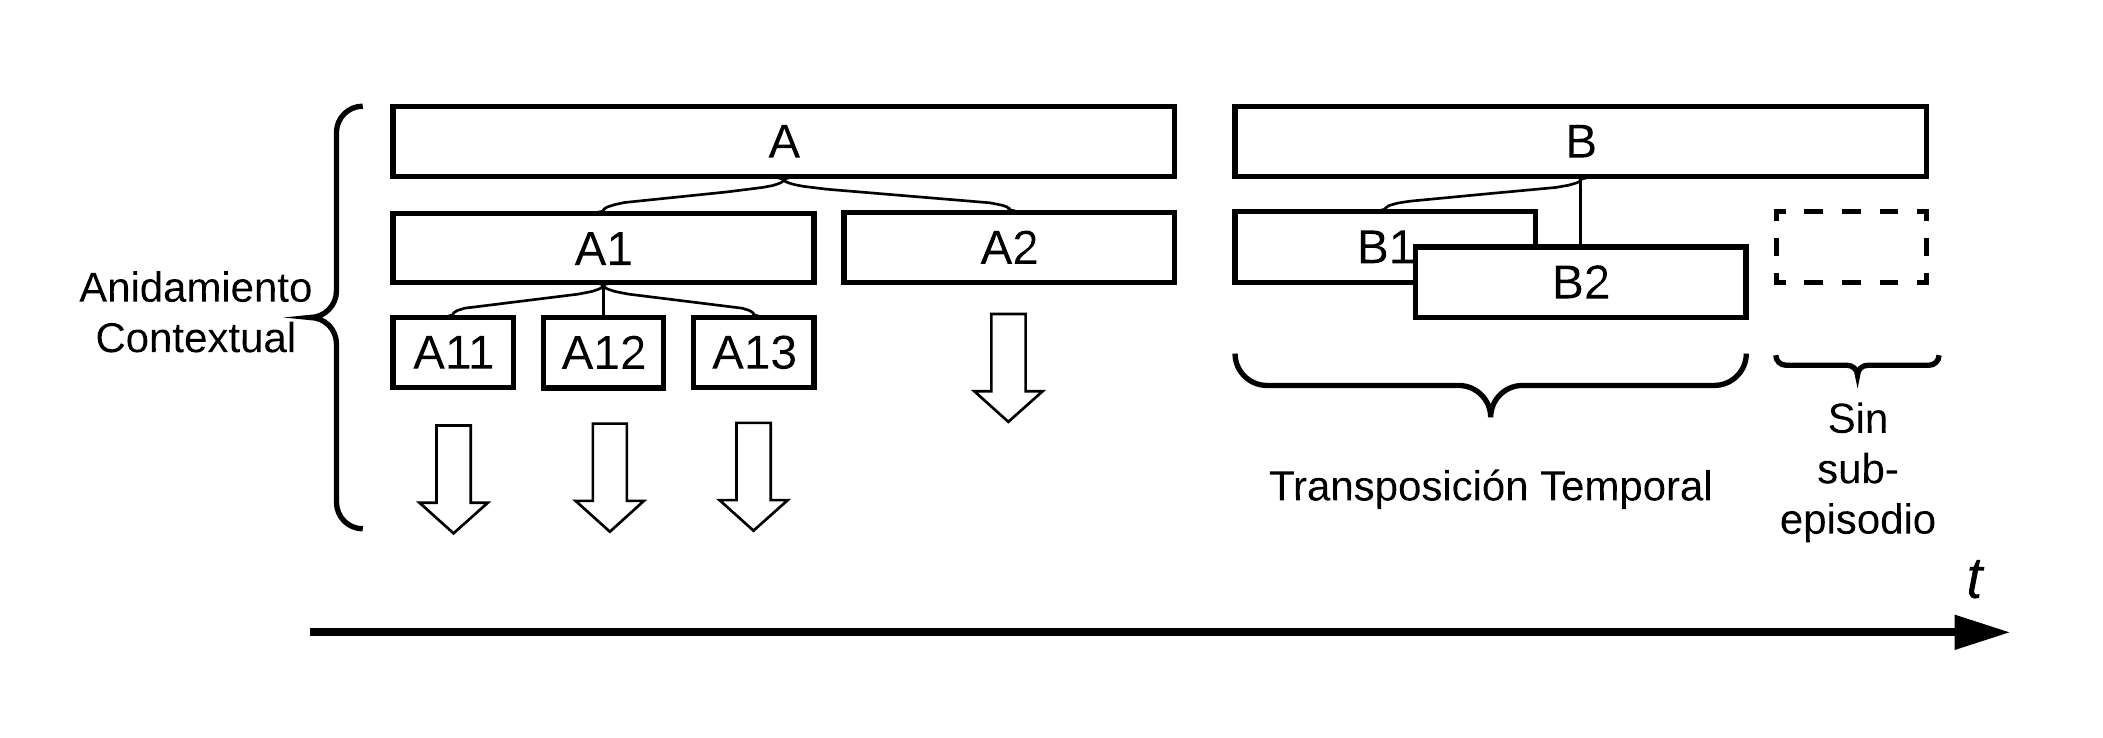
\includegraphics[width=\textwidth]{episodes.png}
	\caption[Concepto de anidamiento y transposición episódica.]
	{\small Diagrama temporal ejemplificando nociones de anidamiento y transposición episódica. Cada cuadro es un episodio identificado por el nombre indicado (\textit{A, B, A1}, \ldots). El tiempo transcurre horizontalmente hacia la derecha, por lo que \textit{A2} ocurre después de \textit{A1}, y \textit{B2} inicia después que \textit{B1}, pero ocurren simultáneamente por un periodo. Los episodios pueden ser anidados indefinidamente.}
	\label{img:episodes}
\end{figure}

% SOBRE TEMPORALIDAD
\ltmconcept{Temporalidad}
Para el árbol episódico es fundamental que cada episodio padre inicie antes que cualquiera de sus hijos, y termine después que todos ellos. Lo anterior es presentado en el diagrama de la Figura~\ref{img:episodes}, donde el episodio \textit{A} cubre el rango temporal de sus hijos. Además, el diagrama ejemplifica un caso particular, denominado \textit{transposición temporal episódica}, donde dos episodios (\textit{B1} y \textit{B2}) ocurren de manera simultánea, cada uno representando eventos distintos. Finalmente, el diagrama muestra un caso de borde, donde un padre puede tener lapsos de tiempo sin hijos asociados (cuadro con bordes punteados bajo el episodio \textit{B}).

% SOBRE MANEJO DE INFORMACIÓN EN PADRES E HIJOS
\ltmconcept{Estrategia de almacenamiento}
Ya que un padre puede ser representado lógicamente por su conjunto de hijos, se decide utilizar una metodología de almacenamiento que no genere redundancia de información. Solo las hojas del árbol son las encargadas de manejar la información semántica del episodio (datos para el campo \textit{What}), lo que potencialmente corresponde a una gran cantidad de datos. Asimismo, las hojas son encargadas de manejar la mayor cantidad de información episódica que sea posible (datos para los campos \textit{When}, \textit{Where} y las relevancias episódicas). Por lo tanto, los nodos internos del árbol (en adelante, \textit{nodos}) manejan poca información y la mayor parte de sus datos puede ser calculada a partir de sus hijos y de manera automática por el servidor. Las estrategias de almacenamiento y reconstrucción para cada tipo de dato serán explicadas en las siguientes secciones. 

% SOBRE EL CONTEXTO
\ltmconcept{Noción de contexto}
Es importante enfatizar que no basta que un episodio esté embebido temporalmente en otro para ser considerado un hijo. Pues a pesar de cumplir la condición de temporalidad, puede ocurrir el caso de que ambos episodios sean simultáneos (ver \RSlabel{12}), pero estén ligados a un contexto distinto. Por ejemplo, durante los días de la competencia RoboCup, el robot podría ser utilizado para una tarea de uno de los estudiantes; a pesar de que los eventos son simultáneos, se puede decir que el último pertenece a otro contexto y debe ser almacenado en un árbol distinto. Esta noción de contexto es importante, y es la razón por la que el servidor debe manejar una cantidad indefinida de árboles episódicos, cada uno identificado por su raíz. Debido lo anterior, cada episodio debe ser almacenado indicando quien es el padre asociado.



%% =============================================================================
%% =============================================================================
%% =============================================================================
\subsection{Contexto temporal: \textit{When}}\label{sec:design_ep_when}
%% =============================================================================
%% =============================================================================
%% =============================================================================

% SOBRE LOS REQUISITOS
\ltmconcept{Requisitos}
De acuerdo al requisito \RSlabel{03}, los episodios deben almacenar información que indique su contexto temporal (\textit{When}), es decir, cuándo  sucedió. Para esto, la única información de interés a almacenar son los instantes de tiempo que indican el fin y el inicio del episodio.

% SOBRE MANEJO DE INFORMACIÓN
\ltmconcept{Estrategia de almacenamiento}
En el caso de las hojas, basta utilizar los instantes de tiempo obtenidos al iniciar y finalizar el episodio. Sin embargo, para el caso de los nodos, se pueden seguir dos estrategias: Utilizar los instantes de tiempo iniciales y finales percibidos, o calcular automáticamente los tiempos de inicio y fin para ajustarse a los hijos. A pesar de que la segunda opción suena razonable, está asumiendo que siempre existirá un hijo para cada instante de tiempo de vida del padre, lo que puede no ser cierto. Por lo tanto, se deben manejar cuidadosamente los valores de tiempo de los padres, para asegurar que no son sobre-escritos por sus hijos, y para asegurar que los padres siempre contienen temporalmente a cada hijo.



%% =============================================================================
%% =============================================================================
%% =============================================================================
\subsection{Contexto espacial: \textit{Where}}\label{sec:design_ep_where}
%% =============================================================================
%% =============================================================================
%% =============================================================================


% SOBRE LOS REQUISITOS
\ltmconcept{Requisitos}
De acuerdo al requisito \RSlabel{04}, los episodios deben almacenar información que indique su contexto espacial (\textit{Where}), es decir, dónde sucedió. A continuación se explican las decisiones de diseño consideradas.

% SOBRE DURACIÓN DE EPISODIOS Y VECTORES
\ltmconcept{Desplazamiento durante episodios}
En primer lugar, dependiendo de la duración del episodio, el robot puede haber estado en más de un lugar durante ese periodo. Esto no es válido solo para episodios nodo, sino que también para hojas, cuando estas representan acciones de desplazamiento del robot. Luego, es importante que cada episodio registre cada uno de los lugares en los que ha estado el robot. El listado de lugares debe ser almacenado ordenadamente y con la hora asociada a cada desplazamiento, lo que es importante por dos motivos: permite calcular la secuencia de movimientos para los padres, y permite reconstruir la ruta del robot durante cada episodio. Para ello, la posición del robot puede ser consultada periódicamente en busca de cambios, para almacenar solo los instantes que indiquen movimiento. 

% SOBRE USO DE AMBAS OPCIONES: Lugares y coordenadas
\ltmconcept{Estrategias de almacenamiento}
La información espacial puede ser manejada de dos maneras: se pueden almacenar los nombres de los lugares en donde el robot estuvo durante el episodio, o se puede almacenar la ubicación precisa del robot durante el episodio, mediante posiciones relativas a un sistema coordenado predefinido. La decisión sobre cual sistema utilizar depende mucho del contexto en el cual funciona el robot. Por ejemplo, en el caso de Bender, hay ocasiones en donde solo es posible conocer su ubicación respecto a un sistema coordenado, mientras que en otras oportunidades, solo se tiene conocimiento verbal de esta. Luego, ya que no existe un consenso sobre que opción es la mejor, y para evitar limitar la usabilidad del sistema LTM, se decide dar soporte a ambas alternativas.


% OPCIÓN SEMÁNTICA
\ltmconcept{Estrategia 1 - Descripción}
Los nombres de lugares en los que estuvo el robot durante el episodio pueden ser almacenados utilizando vectores de \textit{strings}. Considerando el ambiente en donde puede desempeñarse un robot de servicio doméstico, se decide almacenar esta información en dos niveles de profundidad. El primer nivel corresponde a una descripción específica de la ubicación del robot (e.g., ``Comedor''), mientras que el segundo sirve para almacenar el nombre del área donde se encuentra la primera ubicación (e.g., ``Casa de John''), junto a otras de similar orden semántico. En el caso de los episodios nodo, se ha decidido calcular automáticamente toda esta información a partir de sus hijos.

% OPCIÓN COORDENADAS
\ltmconcept{Estrategia 2 - Coordenadas}
Similarmente al caso anterior, las coordenadas de lugares son almacenadas en vectores de puntos, junto con su hora y sistema de coordenadas asociados. Además, para cada punto se debe almacenar el nombre del mapa en donde se define el sistema coordenado. Ya que el trabajo está orientado a robots de servicio doméstico, se ha decidido implementar solamente ubicaciones en 2 dimensiones, es decir, cada punto solo considera 2 valores numéricos. En el caso de los padres se sigue la siguiente estrategia: las posiciones son obtenidas a partir de sus hijos, se agrega un campo para almacenar la envoltura convexa de todas las posiciones, y se agrega un campo indicando el centroide de esta. La envoltura convexa es agregada por motivos prácticos, pues puede ser utilizada para visualización y análisis del árbol episódico.

% LIMITANTES
\ltmconcept{Limitantes} En la Sección \ref{sec:design-limits} se describen dos limitantes del diseño realizado: la posible redundancia de información, y la utilidad de esta.

%% =============================================================================
%% =============================================================================
%% =============================================================================
\subsection{Memoria semántica: \textit{What}}\label{sec:design_ep_what}
%% =============================================================================
%% =============================================================================
%% =============================================================================

% REQUISITOS
\ltmconcept{Requisitos}
De acuerdo a los requisitos \RSlabel{01}, \RSlabel{02}, la memoria semántica (\textit{What}) ligada a un episodio permite describir ``qué'' sucedió en él. Esta debe poder  contener cualquier dato, por lo que no es posible establecer de antemano qué información y estructura debe ser utilizada, sino que esto debe poder ser definido por el usuario. El requisito \RSlabel{07} (regla de flexibilidad episódica) establece que cada episodio debe permitir crear nuevos datos semánticos o actualizar los ya existentes. El requisito \RSlabel{10} (regla de perspectiva episódica) exige que al leer un episodio, este pueda describir sus datos semánticos asociados, de acuerdo a la misma perspectiva que se tenía de ellos cuando el episodio fue ejecutado.

% SEPARACIÓN DE CONCEPTOS
\ltmconcept{Streams y entidades}
La memoria semántica maneja entidades conocidas por el robot e información sobre ellas. Por ejemplo, se puede definir la entidad ``persona'' y almacenar datos como su nombre, nacionalidad o la fecha de la última interacción registrada. Sin embargo, existe un tipo de información que no está asociada a alguna entidad en particular, correspondiente a datos en forma de flujos de información (\textit{streams}). Estos permiten registrar secuencias de imágenes, sonido y otros conceptos basados en flujos de datos percibidos por el robot, especialmente los obtenidos directamente desde sus sensores. Otra característica de los \textit{streams}, es que a diferencia de las entidades, representan datos que no se desea actualizar posteriormente, pues almacenan una fotografía de lo percibido en el instante, la que generalmente es invariable. Entonces, se decide separar la memoria semántica en dos componentes, \textit{streams} y entidades, lo que permite diseñar estrategias de procesamiento adecuadas al funcionamiento de cada uno. 


% GENERALIZANDO MEMORIA SEMÁNTICA
\ltmconcept{Generalización}
Ya que los contenidos a almacenar deben poder ser definidos por el usuario, se establecen las siguientes decisiones de diseño. En primer lugar, el usuario debe definir qué información utilizará, mediante uno o más mensajes de ROS. Segundo, a partir del requisito \RSlabel{18}, debe haber una conexión bidireccional entre los mensajes y los episodios, esto es válido tanto para \textit{streams} como entidades:
\begin{itemize}
\item Mensajes deben tener una referencia al identificador del episodio relacionado.
\item Mensajes deben definir un campo para almacenar su identificador único, el que debe ser utilizado por el episodio.
\end{itemize}

% SOBRE PLUGINS
\ltmconcept{Sistema de plugins}
Se decidió utilizar un sistema basado en plugins para manejar los mensajes ROS definidos por el usuario. De esta manera, se delega al usuario la implementación de los algoritmos para adquisición de la  información semántica y procesamiento de esta. El diseño del servidor LTM en la Sección~\ref{sec:design-server} especifica qué funcionalidades deben ser implementadas por plugins destinados a \textit{streams} o entidades. 

% SOBRE STREAMS
\ltmconcept{Datos semánticos - Streams}
Los \textit{streams} corresponden a flujos de datos generalmente invariables, relacionados a un episodio según sus tiempos de inicio y fin. Existen 3 metodologías para almacenar los \textit{streams}, con ventajas y desventajas. En cada caso, no se requiere almacenar datos cuando no hay episodios activos:
\begin{enumerate}
	\item Cada \textit{stream} contiene solo 1 dato semántico, por lo que no tiene duración y es asociado a un instante de tiempo. Esta estrategia es ideal funcionalmente, pero ya que la tasa de mensajes a almacenar puede ser alta, en la práctica esta solución es costosa en términos de consultas a la base de datos.
	\item Mantener 1 \textit{stream} por cada episodio, con tiempos de inicio y fin idénticos a los del episodio relacionado. Tiene la desventaja de almacenar información duplicada cuando existe traslape temporal de episodios.
	\item Similar a la estrategia anterior, pero subdividiendo el \textit{stream} cuando hay traslape de episodios. Evita la duplicación de información, pero complica la mantención de la base de datos.
\end{enumerate}

Para acotar el trabajo, y bajo la suposición de que en la práctica existen pocos episodios traslapados, se escoge la segunda estrategia. Entonces, cada episodio puede estar asociado a un \textit{stream} de cada tipo, y a su vez, cada \textit{stream} puede contener uno o más datos. El servidor debe proveer notificaciones para indicar el inicio y fin de un episodio, mientras que el usuario debe definir su estrategia para adquirir datos durante ese lapso de tiempo. Por ejemplo, en el caso de un \textit{stream} de imágenes representando la visión del robot, y cuyo fin solo sea de visualización a futuro, el usuario podría almacenar una imagen cada 3 segundos. 

Según la cantidad de plugins a utilizar y la periodicidad de recopilación de información, el espacio de disco requerido para almacenar los mensajes puede ser agotado rápidamente. Para solucionar esto hay 3 alternativas. En primer lugar, se puede expandir la memoria disponible, lo que no es una solución real. En segundo lugar, está el ``olvido'' de información, mediante la eliminación de datos antiguos o de baja relevancia episódica (posiblemente previo respaldo en otra máquina) o eliminar datos intercaladamente. La tercera opción es la degradación de información, para lo que cada usuario debe implementar un algoritmo que disminuya el tamaño de sus mensajes (e.g., disminuyendo la resolución o cantidad de las imágenes del episodio). Ya que las dos primeras opciones pueden ser ejecutadas manualmente por el usuario, se ha decidido utilizar la degradación de mensajes. Esta estrategia puede ser aplicada automáticamente a mensajes antiguos y de baja relevancia episódica.

% SOBRE ENTIDADES
\ltmconcept{Datos semánticos - Entidades}
El usuario debe definir cada tipo de entidad disponible a través un mensaje ROS. Cada tipo (e.g., ``persona'') puede tener muchas instancias (e.g., ``Carl'' y ``Lenny''). A diferencia de los \textit{streams}, las entidades manejan datos modificables, lo que introduce dos condiciones:
\begin{itemize}
\item Su modelo de datos debe soportar el requisito \RSlabel{07} al crear nuevas instancias o modificar una ya existente.
\item El modelo de datos debe soportar el requisito \RSlabel{10}, por lo que cada episodio debe almacenar referencias a las instancias modificadas y los cambios aplicados.
\end{itemize}

Las instancias de una entidad y sus modificaciones no están ligadas a un episodio particular, sino que a los episodios activos durante el registro de la modificación. Entonces, es posible registrar cambios a entidades a pesar de no haber episodios activos.


%% =============================================================================
%% =============================================================================
%% =============================================================================
\subsection{Relevancia generalizada}
%% =============================================================================
%% =============================================================================
%% =============================================================================

% RELEVANCIA GENERALIZADA
\ltmconcept{Requisitos}
De acuerdo a los requisitos \RSlabel{19}-\RSlabel{20}-\RSlabel{21}, los episodios deben almacenar información de relevancia episódica. Estos indicadores son importantes al momento de buscar episodios, para poder ordenarlos de acuerdo a una medida de importancia, y así tener una pista sobre en cuales enfocar la atención. El sistema debe soportar, al menos, la noción de relevancia histórica y emocional, considerando que en un futuro se podrían agregar otros indicadores de relevancia. También, el sistema debe proveer un indicador generalizado, capaz de representar la relevancia global del episodio, mediante un solo indicador numérico que unifique las subrelevancias.

% MANEJO DE INDICADORES
\ltmconcept{Estrategia de almacenamiento}
Entonces, se define la siguiente estrategia de almacenamiento. Cada tipo de indicador debe proveer un valor numérico en el rango $[0, 1]$, que represente la importancia del episodio de acuerdo a su perspectiva. Un valor de 0 significa que el episodio no es relevante, mientras que el valor 1 es utilizado para indicar que el episodio es muy importante. Utilizando el formato anterior, se construye el indicador de relevancia generalizada a partir de todas las subrelevancias definidas para el episodio. Este indicador debe ser actualizado cada vez que una subrelevancia sea modificada o ingresada.

% COMPUTO BASADO EN ALGORITMO X
\ltmconcept{Cómputo}
Este trabajo solo considera dos subindicadores, histórico y emocional, por lo que se decidió utilizar la metodología propuesta por Dood et al. y explicada en la Sección~\ref{sec:theory-modulation}.


%% =============================================================================
%% =============================================================================
%% =============================================================================
\subsection{Relevancia emocional}\label{sec:design_ep_rel_emo}
%% =============================================================================
%% =============================================================================
%% =============================================================================

% RELEVANCIA EMOCIONAL
\ltmconcept{Requisitos}
El requisito de sistema \RSlabel{19} exige el manejo del concepto de relevancia emocional, como un medio para almacenar las emociones ``que siente'' el robot durante un episodio, en conjunto a un indicador de la intensidad de estas.


% ABSTRACCIÓN DEL SISTEMA DE EMOCIONES
\ltmconcept{Abstracción del sistema emocional}
Según se revisó en la Sección~\ref{sec:theory-modulation}, existen diversos sistemas para la generación de emociones y no existe una metodología única para su implementación: Cada sistema es alimentado con datos diferentes, utilizan algoritmos distintos y proveen salidas distintas. Debido a la generalidad esperada para el trabajo, se propone la siguiente estrategia para la abstracción del sistema emocional a utilizar, que permite delegar la implementación al usuario:
\begin{itemize}
\item Se define un conjunto de 8 emociones base, a partir de las emociones primarias propuestas por Plutchik (ver Sección~\ref{sec:theory-modulation}).
\item Se debe almacenar el nivel de intensidad percibido durante un episodio, para cada una de las 8 emociones.
\item Se utilizará un sistema de plugins, donde el usuario debe implementar el mapeo entre las salidas de su sistema emocional, a la combinación de emociones base disponibles para un episodio.
\end{itemize}

% CAMPOS REQUERIDOS
\ltmconcept{Estrategia de almacenamiento}
Las 8 emociones definidas deben seguir el estándar definido para la representación de relevancias, con valores en el rango $[0, 1]$ indicando la intensidad asociada. La relevancia emocional de cada episodio se asocia a la emoción cuya intensidad sea la de mayor valor. Para el caso de episodios nodo, el registro emocional es calculado automáticamente a partir de los hijos, almacenando los valores máximos para cada emoción.

% METADATOS
\ltmconcept{Metadatos}
Además, para simplificar la introspección de episodios a futuro, se decide agregar metadatos que indican el software emocional utilizado y su versión. Es importante enfatizar que cada metadato solo debe ser utilizado para introspección y no tienen influencia en el cálculo de las relevancias.


%% =============================================================================
%% =============================================================================
%% =============================================================================
\subsection{Relevancia histórica}\label{sec:design_ep_rel_hist}
%% =============================================================================
%% =============================================================================
%% =============================================================================

% SOBRE RELEVANCIA HISTORICA
\ltmconcept{Requisitos}
El requisito \RSlabel{20} exige el manejo del concepto de relevancia histórica, como un medio para indicar la importancia de un episodio, según su edad en la base de datos. 

% ALMACENAMIENTO
\ltmconcept{Estrategia de almacenamiento}
Siguiendo el estándar definido para representación de relevancias, se utiliza un valor numérico en el rango $[0, 1]$, que indica el estado de envejecimiento del episodio. Este valor siempre debe ser inicializado en 1, para decaer hacia 0 con el paso del tiempo.

% MANEJO AUTOMÁTICO DE DATOS HISTÓRICOS
\ltmconcept{Actualización automática}
El valor de la relevancia debe ser manejado automáticamente por el sistema LTM. Se propone disminuir el indicador, según el algoritmo de decaimiento presentado por Dood et al. (ver Sección~\ref{sec:theory-modulation}). Ya que se espera almacenar una gran cantidad de episodios, se propone discretizar la función de decaimiento. Los episodios deben ser actualizados en lapsos cada vez más espaciados en el tiempo (e.g., primero cada 1 día, luego 1 vez a la semana, cada 1 mes, cada 1 año), lo que permite acotar el esfuerzo computacional dedicado a las actualizaciones.


%% =============================================================================
%% =============================================================================
%% =============================================================================
\subsection{Datos para introspección}
%% =============================================================================
%% =============================================================================
%% =============================================================================

% SOBRE RAZONAMIENTO
\ltmconcept{Metadatos}
El último conjunto de datos considerado para un episodio es denominado \textit{Metadatos}. Estos no están ligados a algún requerimiento de software, por lo que no son formalmente necesarios, sin embargo, permiten almacenar datos útiles para la implementación LTM, y sirven para conocer información sobre el software utilizado durante el almacenamiento de cada episodio. Los \textit{Metadatos} tienen como finalidad ser de utilidad al resolver problemas relacionados al sistema LTM, y para cuando los usuarios deseen conocer el contexto de software sobre el cual fue generado el episodio.


%% =============================================================================
%% =============================================================================
%% =============================================================================
\subsection{Limitantes y trabajo futuro}\label{sec:design-limits}
%% =============================================================================
%% =============================================================================
%% =============================================================================

% SOBRE LIMITANTES DEL DISEÑO Y TRABAJO FUTURO
A continuación se presenta un conjunto de limitantes conocidas del diseño episódico desarrollado, las que pueden ser consideradas como parte del trabajo futuro.

% SOBRE COMPLETITUD Y LAPSOS EN BLANCO..
\ltmconcept{Ausencia de hijos}
Este problema fue explicado parcialmente en la Sección~\ref{sec:design_ep_when}, y aparece con padres cuyo rango temporal no es cubierto completamente por sus hijos. Esto puede suceder cuando el usuario decide no almacenar algunos episodios hoja, pues los considera poco relevantes. El efecto de esto, es que los padres podrían contar con información incompleta al calcular datos a partir de sus hijos. Se puede argumentar que, ya que el usuario considera que los subepisodios eran irrelevantes, entonces la información perdida también lo es. Sin embargo, por motivos de introspección, puede ser de interés almacenar los datos de \textit{streams} asociados a los periodos temporales perdidos.

\ltmconcept{Episodios de larga duración}
A pesar de que el diseño permite episodios de duración indefinida, en la práctica es raro que el robot funcione por periodos prolongados. Luego, los episodios cuyo fin es dar un contexto temporal a un árbol episódico no pueden ser almacenados directamente (e.g., cuando el robot está participando en una competencia de 4 días de duración). A pesar de lo anterior, el diseño permite la introducción manual de episodios de larga duración, sin tener que mantener en funcionamiento el robot durante todo el periodo.

\ltmconcept{Memoria emocional detallada}
Ya que el diseño apunta a ser lo suficientemente genérico, la información emocional que se puede exigir es acotada. El formato permite almacenar los datos justos para la asignación de relevancias, pero a la vez, limita las consultas posibles sobre las emociones del robot en un episodio. Particularmente, en episodios de larga duración sería interesante conocer la secuencia (ordenada) de emociones, o las causas de estas. A pesar de que el diseño no almacena información al respecto, si permite definir una forma alternativa de almacenar tales datos. Se puede crear una entidad ``Robot'' con campos asociados a sus emociones, para así, llevar un registro detallado de lo que se necesite.

\ltmconcept{Ubicación del robot duplicada o no útil}
Se cree que el formato propuesto para el campo \textit{Where} se ajusta a los requerimientos de un robot doméstico, sin embargo, se identifican dos problemas. Por un lado, la naturaleza de la ubicación del robot no depende de un episodio, sino que es información desacoplada de este, similar al funcionamiento de una entidad. Esto genera duplicación de la información en caso de traslape episódico. Por otro lado, se cree que el formato se adapta a los requerimientos para Bender, pero pueden haber usuarios que requieran almacenar otra información (e.g., GPS) o utilizar mayores niveles de profundidad semántica (e.g., Chile $\rightarrow$ Santiago $\rightarrow$ Laboratorio $\rightarrow$ Mesón A). En un trabajo futuro se podría modificar el diseño, para manejar el campo \textit{Where}  de manera similar al caso de las entidades, donde cada usuario defina los datos que desea almacenar y su metodología de adquisición mediante un plugin asociado, y asimismo, evitando la redundancia de información.

%% =============================================================================
%% =============================================================================

%% =============================================================================
%% =============================================================================

%% =============================================================================
%% =============================================================================

%% =============================================================================
%% =============================================================================
%% =============================================================================
\section{Diseño del Modelo de Datos}\label{sec:data_model_design}
%% =============================================================================
%% =============================================================================
%% =============================================================================

En esta sección se presentan las decisiones sobre el diseño del modelo de datos a utilizar para el trabajo. En primer lugar, se revisan las consideraciones sobre la base de datos escogida: \textit{MongoDB}. Luego, se describe el manejo de mensajes episódicos y sus datos semánticos asociados: \textit{streams} y entidades.


%% =============================================================================
%% =============================================================================
%% =============================================================================
\subsection{Base de datos}
%% =============================================================================
%% =============================================================================
%% =============================================================================

% SOBRE SELECCIÓN DE MONGO DB
\ltmconcept{MongoDB}
De acuerdo al diseño de los mensajes episódicos, la implementación del sistema LTM requiere el manejo de datos no conocidos de antemano, sino que representados mediante mensajes de ROS que debe definir el usuario. Además, el sistema debe permitir modificar la representación de tales mensajes a futuro y soportar el almacenamiento de datos binarios. Por lo tanto, se decidió utilizar la base de datos no relacional \textit{MongoDB}, presentada en la Sección~\ref{sec:mongodb}. 

La decisión sobre el uso \textit{MongoDB} se basa en tres razonamientos principales. Primero, \textit{MongoDB} ya es de uso extendido en la comunidad ROS, por lo que ya ha sido probada y está disponible en muchos robots de servicio domésticos, evitando agregar dependencias extra a tales trabajos. Además, la interfaz ROS para esta es considerada estable, al menos hasta el año 2023.  Finalmente, \textit{MongoDB} se ocupa actualmente en el robot Bender. Así, se minimizan los problemas de dependencias y compatibilidad a futuro.


% SOBRE SEPARACIÓN DE COLECCIONES
\ltmconcept{Colecciones}
Debido al funcionamiento de \texttt{warehouse\_ros\_mongo}, visto en la Sección \ref{sec:mongodb}, cada mensaje ROS debe ser asociado a una colección distinta. Particularmente, una colección será destinada al almacenamiento de episodios, mientras que cada mensaje definido por el usuario será asociado a una colección diferente. En primera instancia, la base de datos no relacional permitiría almacenar todos los mensajes en la misma colección, pero la separación de cada tipo de dato en colecciones diferentes es conveniente por las siguientes razones:
\begin{itemize}
\item Permite optimizar las consultas simples a la base de datos, que no requieran acceder a toda la memoria semántica asociada.
\item Se evita propagar problemas al registro de episodios, cuando se presenten fallos en los plugins de memoria semántica implementados por el usuario.
\item Ya que el sistema debe soportar una cantidad indefinida de mensajes ROS elegidos por el usuario, se evita saturar el registro de episodios con mensajes que, una vez agrupados, superen el límite de tamaño (16MB) permitido a cada elemento de una colección.
\end{itemize}

% REQUISITO DE MODIFICACIÓN DE REPRESENTACIÓN
\ltmconcept{Modificación de mensajes semánticos}
El requisito \RSlabel{14} especifica que el servidor debe permitir modificar la representación de los mensajes episódicos almacenados. Esto puede suceder porque el usuario decide agregar/quitar campos al mensaje, o porque una dependencia del mensaje fue actualizada. La implementación debe soportar la migración desde la estructura antigua a la nueva.

%% =============================================================================
%% =============================================================================
%% =============================================================================
\subsection{Colección de episodios}
%% =============================================================================
%% =============================================================================
%% =============================================================================

Todos los episodios, definidos por su mensaje ROS, serán almacenados en la colección \texttt{episodes}. De acuerdo a los requisitos \RSlabel{05} y \RSlabel{22}, cada episodio debe ser indexado al menos por los campos \textit{What}, \textit{When}, \textit{Where}, las relevancias emocionales y sus campos internos. En el caso de \textit{What}, las entidades y \textit{streams} también deben ser indexados, y queda a criterio del usuario cuales campos son de interés para cada concepto.

%% =============================================================================
%% =============================================================================
%% =============================================================================
\subsection{Colecciones de streams}
%% =============================================================================
%% =============================================================================
%% =============================================================================

\ltmconcept{Colección}
Según se explicó anteriormente, cada \textit{stream} definido por el usuario es asociado a una colección de \textit{MongoDB} propia. El nombre de cada colección lleva el prefijo \texttt{stream:}, seguido de un identificador definido por el usuario.

\ltmconcept{Estrategia}
Por cada episodio a almacenar se genera un \textit{stream} de cada tipo disponible, para ser almacenado en su colección respectiva. Esto se ejemplifica en la Figura~\ref{img:episodes-and-semantic-data}, mediante un diagrama comparando la relación entre un episodio y los datos semánticos percibidos, de acuerdo al diseño episódico descrito en la Sección~\ref{sec:design_ep_what}.

\begin{figure}[!ht]
	\centering
	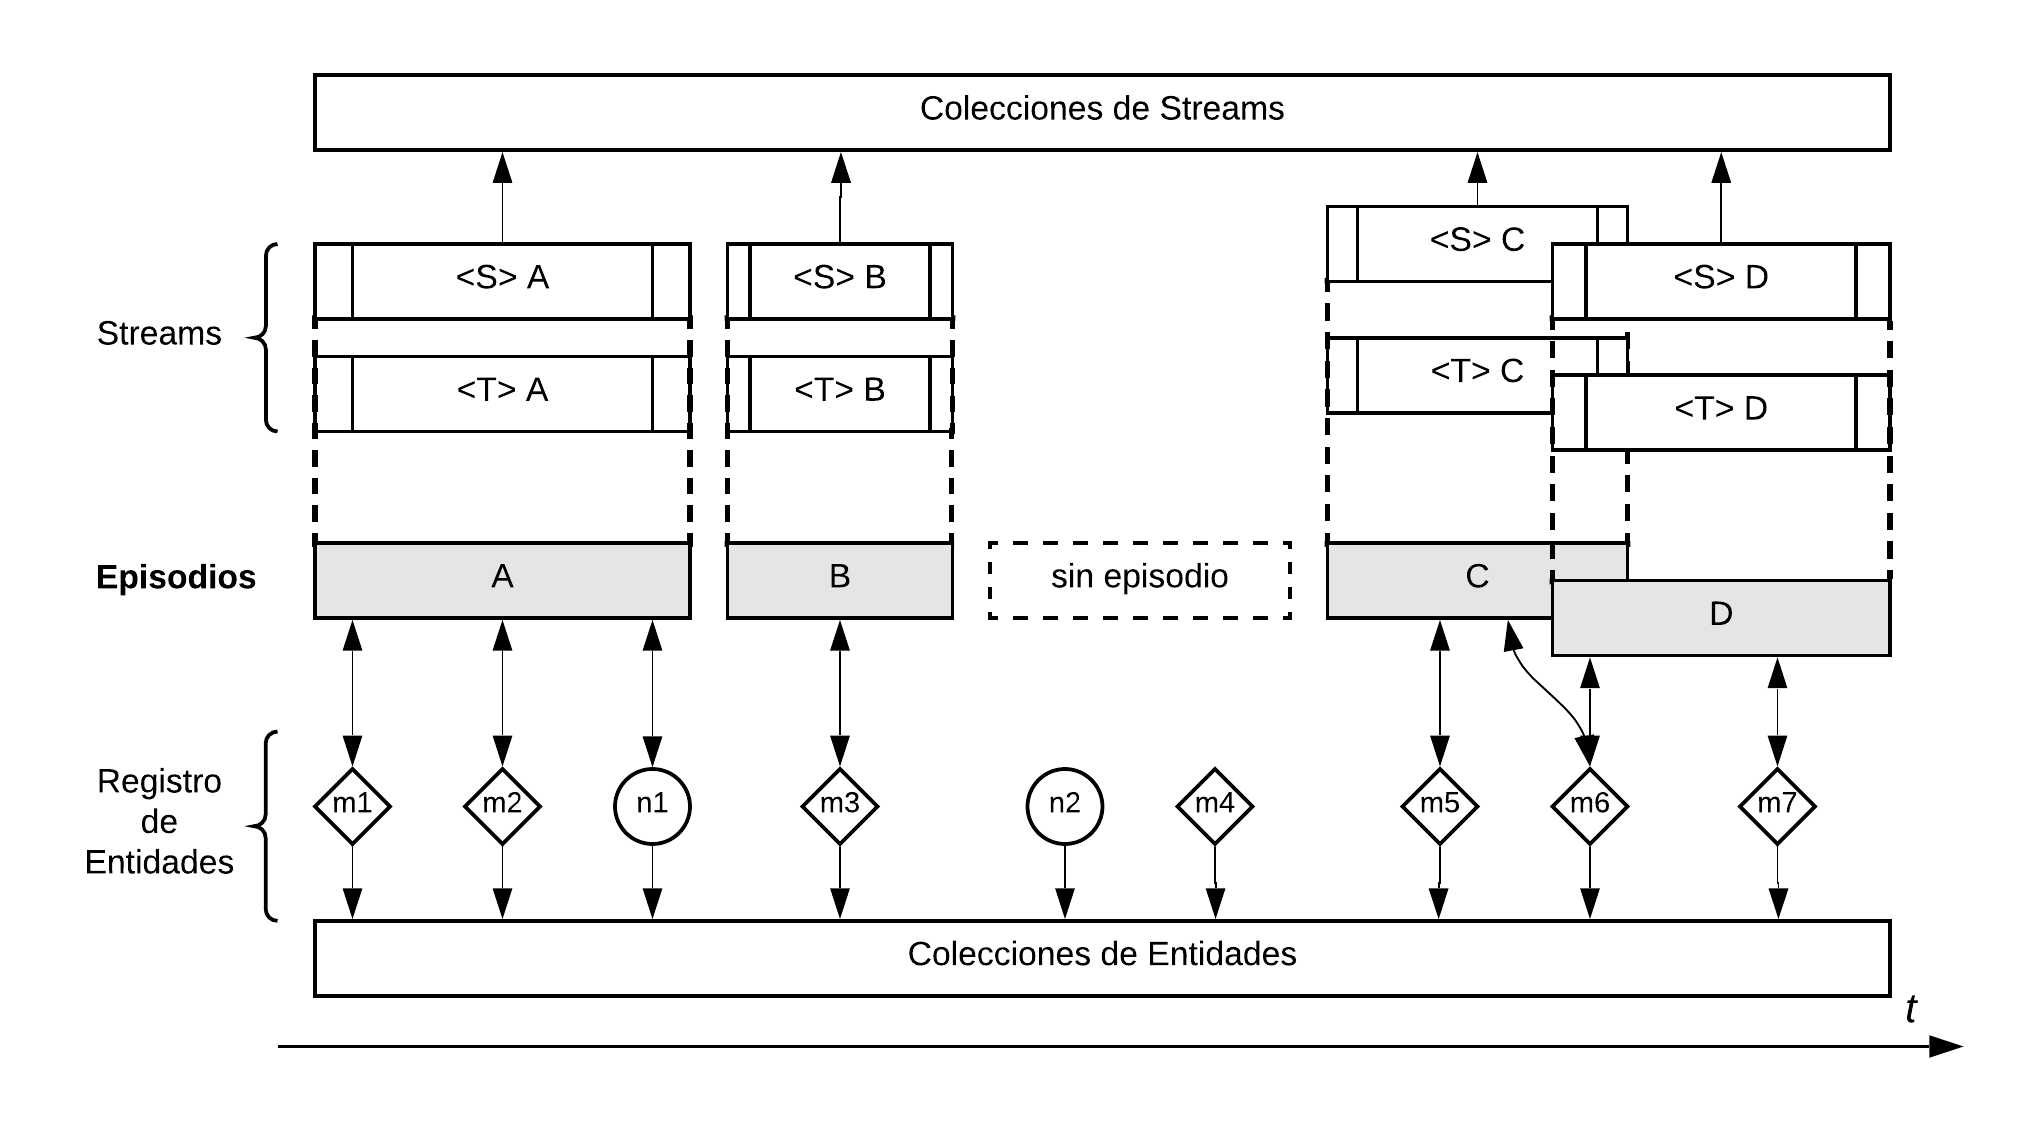
\includegraphics[width=\textwidth]{episodes-and-semantic-data.png}
	\caption[Funcionamiento de \textit{streams} y entidades respecto a los episodios.]
	{\small Funcionamiento de \textit{streams} y entidades respecto a los episodios. \texttt{\textless S\textgreater} y \texttt{\textless T\textgreater} hacen referencia a 2 tipos de \textit{streams}, mientras que \texttt{$m_1\ldots m_7$} (rombos) y \texttt{$n_1, n_2$} (círculos) son notificaciones sobre cambios a las entidades \textit{m} y \textit{n}. Un \textit{stream} de cada tipo es asociado a cada episodio, incluso en caso de transposición. Cada notificación sobre entidades es asociada a todo episodio activo. En caso de no haber episodio, no se almacenan \textit{streams}, pero si se registran los cambios en entidades.}
	\label{img:episodes-and-semantic-data}
	\end{figure}


\ltmconcept{Indexado}
Por lo general, los campos de un \textit{stream} no requieren ser indexados, ya que es conveniente almacenarlos de manera binaria. Sin embargo, durante la implementación del plugin asociado, el usuario puede decidir añadir metadatos para indexar campos convenientes. La utilidad de esto, es que permitirá agregar nuevos términos de comparación para las consultas a la base de datos. Luego, se tienen dos formas de acceder a un \textit{stream} en particular; mediante su mensaje episódico asociado, o a través de los metadatos definidos por el usuario.

\ltmconcept{Tamaño del mensaje}
El límite de tamaño para cada mensaje ROS a almacenar es de $16 MB$, lo que impone una cota superior a la cantidad de datos que pueden ser almacenados por cada episodio. Según se describe en la Sección~\ref{sec:mongodb}, \textit{MongoDB} provee estrategias de almacenamiento para sobrepasar este límite.

%\todoimprove{Por ejemplo, esto permitiría almacenar hasta $N$ imágenes a color de cierto tamaño, o $M$ de ellas en escala de grises.}


%% =============================================================================
%% =============================================================================
%% =============================================================================
\subsection{Colecciones de entidades}
%% =============================================================================
%% =============================================================================
%% =============================================================================

\ltmconcept{Colección}
Cada mensaje ROS definido por el usuario para representar una entidad de la memoria semántica, es asociado a una colección de \textit{MongoDB} propia. El nombre de cada colección lleva el prefijo \texttt{entity:}, seguido de un identificador definido por el usuario. 

\ltmconcept{Flexibilidad}
El modelo debe considerar un identificador único para indicar la instancia de cada entidad. Así, cuando un episodio registra actualizaciones de una instancia particular, modifica su entrada en la colección correspondiente.

\ltmconcept{Perspectiva}
Para soportar este concepto se requiere poder reconstruir el estado de una instancia en cada instante de tiempo desde su creación. Este es un requisito común para una base de datos, denominado \textit{Audit Trail}. La solución propuesta para el problema es la siguiente:
\begin{itemize}
\item Por cada entidad (mensaje ROS) se deben mantener 2 colecciones en la base de datos.
\item Las primera colección almacena un historial de las modificaciones a cada instancia de la entidad. Cada entrada debe indicar el tiempo de ocurrencia, tener referencias a los episodios asociados e indicar los cambios modificados.
\item La otra colección almacena el estado actual de cada instancia de la entidad, lo que es equivalente a aplicar su historial de cambios desde el comienzo. Esta colección tiene el propósito de agilizar consultas que solo requieran los conocimientos actuales de cada instancia.
\end{itemize}
Ya que \texttt{warehouse\_ros\_mongo} solo permite almacenar un tipo de mensaje ROS por colección, la destinada a almacenar los cambios es subdividida en dos colecciones:
\begin{itemize}
\item La primera almacena un mensaje ROS del mismo tipo que la entidad, y sirve para indicar los cambios registrados. Su nombre utiliza el prefijo \texttt{entity:} y el sufijo \texttt{.trail}.
\item La segunda almacena un mensaje ROS con los metadatos necesarios para mantener el historial. Su nombre utiliza el prefijo \texttt{entity:} y el sufijo \texttt{.meta}.
\end{itemize}

\ltmconcept{Estrategia}
Con la finalidad de mantener la consistencia del historial de entidades, se deben almacenar todos los cambios recolectados para una entidad, a pesar de que no haya un episodio activo. Sin embargo, cada registro debe tener referencias a los episodios activos durante el instante de su recolección, y a su vez, cada episodio debe tener referencias a tales registros. Lo anterior es ejemplificado en el diagrama de la Figura~\ref{img:episodes-and-semantic-data}.

\ltmconcept{Indexado}
Se delega al usuario la definición de los campos de interés para el indexado de su mensaje. Estos campos estarán disponibles para realizar consultas episódicas al servidor. Sin embargo, para enriquecer las búsquedas de episodios, los metadatos del registro histórico deben tener vectores con los nombres de los campos modificados, campos creados, y campos eliminados. Los 3 vectores deben estar indexados.


%% =============================================================================
%% =============================================================================
%% =============================================================================
\subsection{Consultas al modelo}
%% =============================================================================
%% =============================================================================
%% =============================================================================

De acuerdo a los requisitos \RSlabel{06} y \RSlabel{17}, el modelo debe soportar operaciones CRUD sobre los episodios y mensajes semánticos almacenados. Las operaciones deben permitir filtrar los episodios mediante condiciones de \{igualdad, mayor/menor que, pertenencia a arreglos\} sobre los campos indexados. Se debe dar soporte para comparaciones entre los siguientes tipos de dato primitivos de ROS: \{\texttt{bool}, \texttt{int}, \texttt{float}, \texttt{string}\} y condiciones de pertenencia a arreglos de esos tipos.

A continuación se describe la estrategia de procesamiento para las consultas CRUD que debe soportar el sistema. En cada caso se enfatizan las reglas a seguir para mantener la consistencia del modelo de datos.

\subsubsection{Operaciones de inserción (Create)}
%% =============================================================================

\ltmconcept{Episodios}
La inserción de episodios se hace en un proceso de dos etapas:
\begin{enumerate}
\item  Al inicio del episodio se declara la creación de este al servidor, el que proveerá un identificador disponible para su registro. Si el usuario indica que se trata de un episodio hoja, el servidor notifica a los plugins relacionados para que recopilen la información episódica y semántica requerida.
\item  Al finalizar el episodio, el usuario debe indicar la referencia al padre. Este proceso notifica a los plugins para que finalicen la recopilación de información y se almacene el mensaje episódico y el \textit{stream} asociado.
\end{enumerate}
Tras la inserción del episodio se deben actualizar todos los padres, hasta llegar a la raíz.

Los requisitos no lo exigen, pero en caso de dar soporte para la inserción de episodios pasados, no se deben ejecutar los plugins episódicos ni semánticos. La información sobre relevancia emocional y posición debe ser entregada por el usuario. El \textit{stream} debe ser insertado manualmente por el usuario. Se deben registrar automáticamente las entidades que calcen con el lapso de tiempo designado. Análogamente, se debe actualizar el árbol episódico, hasta llegar a la raíz.

\ltmconcept{Streams}
Para la inserción de \textit{streams} se debe indicar el episodio asociado e incluir la referencia del \textit{stream} al episodio. En caso de ya existir un \textit{stream} del mismo tipo asociado al episodio, se sobrescribe la referencia y se elimina el antiguo de su colección. Además, es necesario que los tiempos de inicio y fin del mensaje estén dentro de los límites temporales definidos por el episodio.

\ltmconcept{Entidades}
Los requisitos \RSlabel{07} (flexibilidad) y \RSlabel{10} (perspectiva) establecen dos operaciones de inserción sobre entidades: creación de una nueva instancia y la modificación de una instancia ya existente, mediante la inserción de un nuevo registro en el historial. Ambas operaciones son requeridas para registros obtenidos en el instante actual. Ya que la creación de una nueva instancia se puede ver como un caso particular de modificación, solo se detallará la estrategia del último caso:
\begin{itemize}
\item El nuevo registro debe indicar la fecha de creación, un identificador único del historial y una referencia a la instancia que modifica/crea.
\item Se debe modificar/crear la instancia en la colección que mantiene los datos actualizados.
\item La inserción del registro solo debe almacenar los datos que fueron modificados, agregados o eliminados. La información que se mantuvo estática no debe ser registrada.
\item Se deben agregar referencias bidireccionales a los episodios cuyo lapso de vida contenga al registro.
\end{itemize}

No es necesario dar soporte para crear nuevos registros del historial de entidades, asociados a un tiempo pasado. En caso de hacerlo, se debe seguir una estrategia similar a la anterior, pero además modificando recursivamente los registros adyacentes (temporalmente), para mantener la consistencia del historial.

\ltmconcept{API ROS} Las operaciones de inserción de \textit{streams} y entidades son manejadas automáticamente por el sistema LTM, por lo que no es necesario proveer una API para ello. Por otro lado, si se requiere una API para las operaciones de registro e inserción de episodios.

\subsubsection{Operaciones de lectura (Read)}
%% =============================================================================

\ltmconcept{Etapas de consulta}
Para evitar sobrecargar el ancho de banda de red, con respuestas a consultas que retornen muchos episodios o datos semánticos, se diseñan las operaciones de lectura en 2 etapas. Primero, se obtienen los identificadores de los mensajes de interés mediante una condición que provee el usuario. Luego, se puede acceder a los episodios, \textit{streams} y entidades mediante servicios ROS, encargados de retornar mensajes para los identificadores escogidos.

\ltmconcept{Filtro de mensajes}
La búsqueda de mensajes según condiciones es considerada por el requisito \RSlabel{06}.
Para evitar limitar las consultas que puede realizar el usuario sobre la base de datos y para simplificar el diseño, se decide utilizar el sistema de condiciones nativo de MongoDB. Así, es posible aplicar filtros complejos a las consultas, basados en todos los campos disponibles de cada documento. Sin embargo, las consultas solo pueden ser aplicadas a una colección a la vez. Algunas de las condiciones que provee MongoDB son: igualdad, mayor qué (y derivados), pertenencia a un arreglo y agrupamiento lógico mediante condiciones \textit{AND} y \textit{OR}.

\ltmconcept{Episodios}
Se debe proveer un servicio para filtrar episodios de acuerdo a una condición basada en los metadatos disponibles. El servicio debe retornar los identificadores de los episodios que calcen con la condición, junto a los identificadores de los \textit{streams} y entidades asociadas. Además, se debe proveer un servicio para obtener episodios de acuerdo a su identificador.

\ltmconcept{Streams}
De manera similar, se debe proveer un servicio para filtrar \textit{streams} de acuerdo a una condición basada en sus metadatos. El servicio debe retornar los identificadores de los mensajes que cumplan la condición y sus episodios asociados. Además, se debe proveer un servicio para obtener \textit{streams} mediante su identificador.

\ltmconcept{Entidades}
En el caso de las entidades, el filtro debe poder ser aplicado a la colección de entidades actuales y al historial de cambios. La consulta al historial debe permitir filtrar mediante los nombres de los campos modificados, añadidos u olvidados en cada registro. En ambos casos, se deben retornar los identificadores de las entidades o registros que calcen con la condición, sumado a los de los episodios asociados.

Además, se debe proveer un servicio para obtener una entidad según su identificador. Sin embargo, para cumplir con el requisito \RSlabel{10} (perspectiva), la consulta debe permitir indicar una fecha, para retornar la entidad de acuerdo al conocimiento obtenido hasta el momento.

\ltmconcept{API ROS}
De acuerdo a lo anterior, se debe proveer una API ROS para realizar consultas con condiciones en el formato de MongoDB, para las colecciones de episodios, \textit{streams} y entidades. Además, se deben proveer servicios ROS para obtener episodios, entidades y \textit{streams} según sus identificadores.

\subsubsection{Operaciones de actualización (Update)}
%% =============================================================================

\ltmconcept{Episodios}
De acuerdo al requisito \RSlabel{08}, los episodios son únicos y solo tienen una instancia para ser aprendidos. Entonces, a pesar de ser útil, no es necesario proveer servicios para la actualización de episodios. En el caso de hacerlo, se deben modificar todos los nodos padres, hasta llegar a la raíz. En caso de modificar el intervalo de tiempo, se deben actualizar las referencias bidireccionales con las entidades ya existentes. Al acortar el intervalo de tiempo, se debe modificar el \textit{stream} asociado, para eliminar mensajes sobrantes.

\ltmconcept{Streams} De la misma manera, ya que los \textit{streams} hacen referencia a datos estáticos, no es necesario proveer esta funcionalidad para ellos. Solo tiene sentido actualizar el intervalo de tiempo del mensaje cuando el de su episodio relacionado sea modificado.

\ltmconcept{Entidades}
Por otro lado, el requisito de flexibilidad \RSlabel{07} exige que las entidades deban soportar operaciones de actualización. Estas ya son manejadas por el modelo de datos mediante inserciones en las 3 colecciones correspondientes a la entidad, por lo que no hay necesidad de proveer una API con esta funcionalidad.

En caso de proveer una API para actualizar mensajes del historial, las reglas son las siguientes: se deben modificar recursivamente los registros adyacentes del historial, para considerar los cambios; se debe actualizar la colección que mantiene la imagen actual de la instancia; se deben actualizar las referencias bidireccionales con los episodios que ocurrieron en ese lapso de tiempo.

\ltmconcept{API ROS} 
Como se revisó, no es un requisito proveer servicios ROS para la actualización de los episodios y la memoria semántica. De todas formas, tales funcionalidades son soportadas por el modelo de datos, y pueden ser consideradas como parte del trabajo futuro.


\subsubsection{Operaciones de eliminación (Delete)}
%% =============================================================================

A partir de los requisitos de sistema, no es necesario proveer operaciones de eliminación de mensajes episódicos. Sin embargo, esta operación puede ser de utilidad para pruebas o liberación de memoria.

\ltmconcept{Episodios} En el caso de eliminar un episodio, se deben quitar sus referencias de las entidades y eliminar el \textit{stream} relacionado. Además, se deben actualizar todos los padres hasta llegar a la raíz, para quitar la información asociada al hijo modificado.

\ltmconcept{Streams}
Al eliminar un \textit{stream} se debe quitar su referencia del episodio relacionado.

\ltmconcept{Entidades}
Al eliminar algún mensaje del historial de una entidad, se deben quitar sus referencias de los episodios relacionados, es decir, todo episodio cuyo periodo de vida contenga el instante asociado al mensaje. Se debe quitar el registro del historial y actualizar los historiales adyacentes para mantener su consistencia. Se deben recalcular los datos asociados a la entidad actual.

\ltmconcept{API ROS} 
No es necesario proveer una API ROS para la eliminación de información episódica o semántica. Sin embargo, tales funcionalidades son soportadas por el modelo de datos, y pueden ser consideradas como parte del trabajo futuro.

%% =============================================================================
%% =============================================================================

%% =============================================================================
%% =============================================================================

%% =============================================================================
%% =============================================================================

%% =============================================================================
%% =============================================================================
%% =============================================================================
\section{Diseño del Servidor LTM}\label{sec:design-server}
%% =============================================================================
%% =============================================================================
%% =============================================================================

A continuación se describe el diseño del servidor LTM, a partir de las consideraciones para el modelo de datos presentadas en las secciones anteriores. En primer lugar, se revisa el diseño operativo para el manejo de la memoria episódica: la adquisición de episodios, la recolección de información emocional y de ubicación, y el manejo de relevancias episódicas. Luego, se revisa el diseño de la memoria semántica (\textit{streams} y entidades), el manejo de las colecciones, la API ROS y el flujo de información.

El sistema LTM diseñado se presenta en la Figura~\ref{img:diagrama-software}. A modo general, se indican las 3 etapas del flujo de información en el sistema LTM: recopilación desde la memoria STM del robot, manejo y almacenamiento por el servidor, y uso de la información por las aplicaciones del usuario. Los componentes del diagrama son explicados en detalle a continuación.

\begin{figure}[!ht]
	\centering
	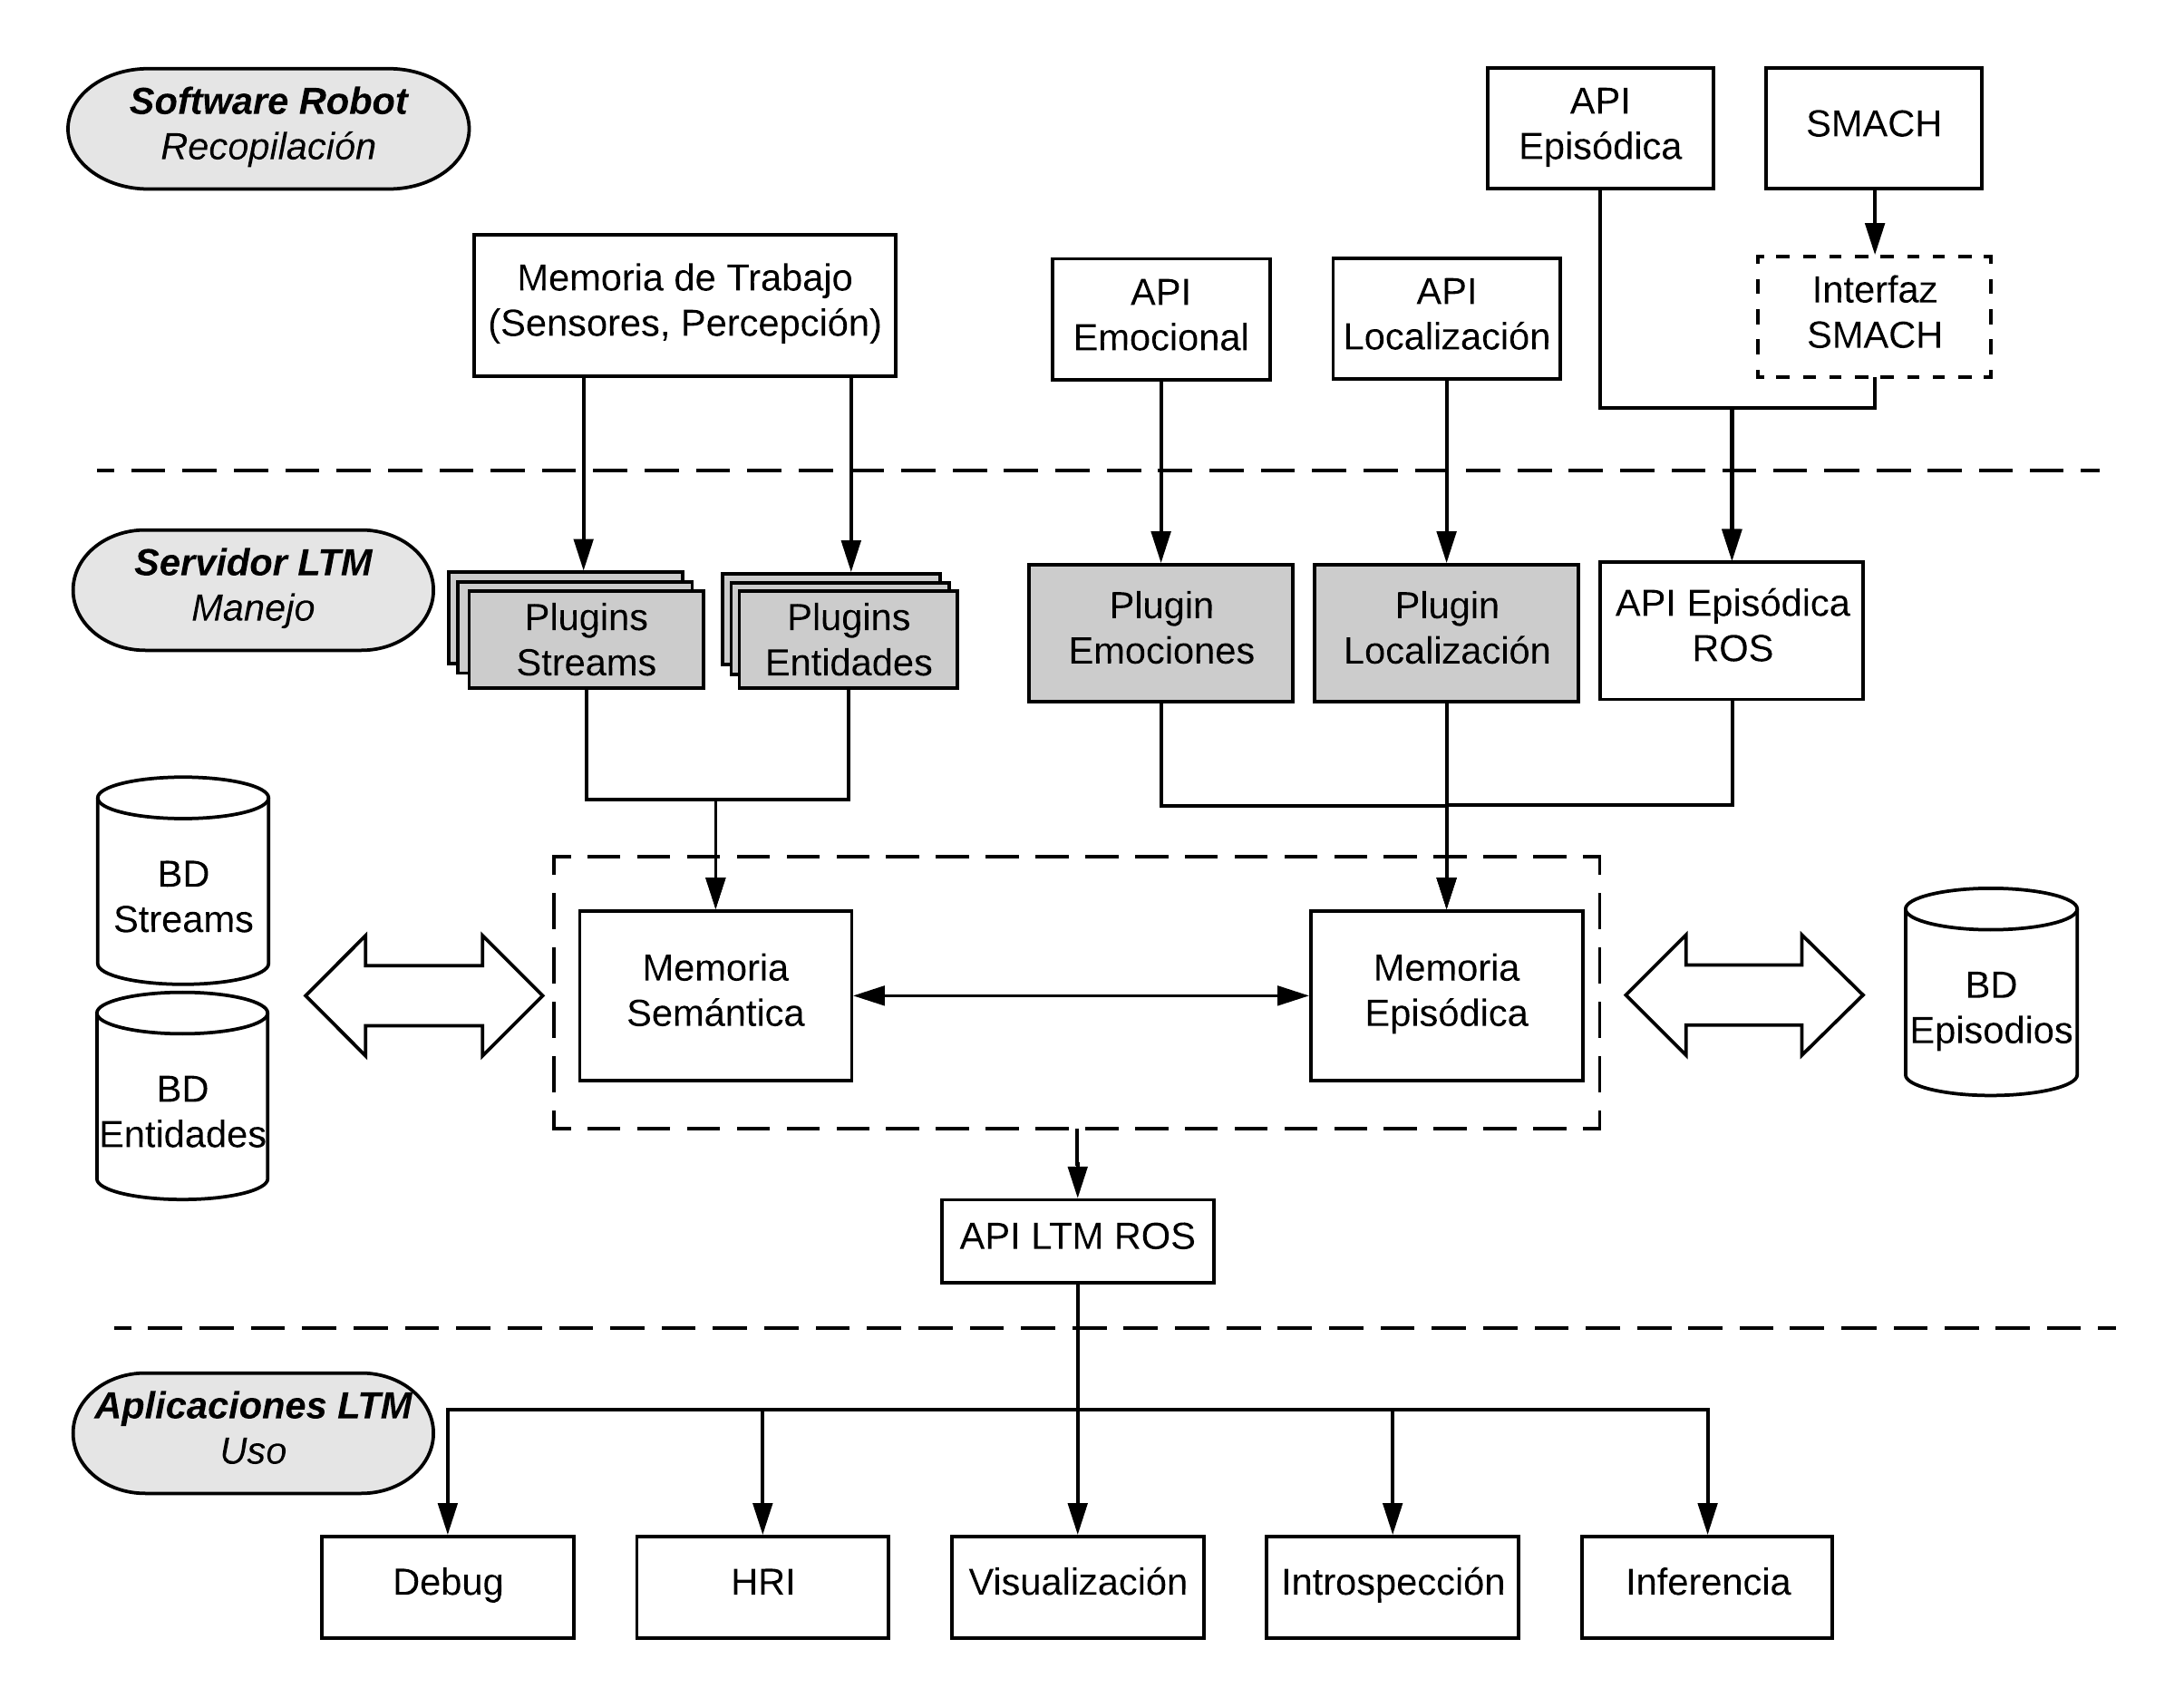
\includegraphics[width=\textwidth]{diagrama-software.png}
	\caption[Diseño del sistema LTM y módulos de software involucrados.]
	{\small Diagrama con el diseño del sistema LTM y los módulos de software involucrados. La zona superior indica todos los módulos de software del robot necesarios para proveer información al sistema LTM. En plomo se presentan los componentes que debe implementar el usuario, que sirven como interfaz entre el robot y el servidor, para la recopilación de información. En la zona central se realiza el manejo y almacenamiento de la información episódica. En la zona inferior, el servidor se comunica mediante una API ROS con las aplicaciones LTM implementadas por el usuario.}
	\label{img:diagrama-software}
\end{figure}


%% =============================================================================
%% =============================================================================
%% =============================================================================
\subsection{Memoria episódica}
%% =============================================================================
%% =============================================================================
%% =============================================================================

En esta sección se describe el diseño del mecanismo para la recolección de episodios, sus datos a partir de plugins y la actualización de relevancias episódicas.

\subsubsection{Recopilación de episodios}

Como se muestra en la Figura~\ref{img:diagrama-software}, el servidor depende de una API episódica para la adquisición de episodios. El diseño propuesto almacena episodios en dos etapas: registro y término, mediante una API ROS basada en servicios. Como lo indica el diagrama, el servidor se comunica con cada plugin para recopilar la información episódica y semántica necesaria.

\ltmconcept{Registro}
En esta etapa, el usuario debe indicar el inicio de un nuevo episodio. Luego, el servidor se encarga de registrar el episodio, generando un identificador único, el que es retornado al usuario. Ya que el sistema debe soportar anidamiento y transposición, pueden haber muchos episodios registrados simultáneamente. 

Durante el registro se debe indicar el tipo de episodio a introducir (hoja o nodo). Si el episodio es de tipo hoja, se notifica a todos los plugins, para que consideren el nuevo episodio como activo e inicien las tareas de recopilación de información. De acuerdo al diseño episódico, no se debe recopilar información para episodios nodo.

\ltmconcept{Término}
Una vez que el episodio ha concluido, el usuario debe notificar al servidor sobre esto, indicando el identificador del padre, los \textit{tags} asociados y los metadatos episódicos que desee almacenar.

Tras recibir la notificación, el servidor recolecta información episódica desde cada plugin, almacena el episodio en la base de datos y lo marca como inactivo. En caso de ya no haber episodios activos, cada plugin es notificado para dejar de recopilar información.


\subsubsection{Plugin: \textit{Where}}
%% =============================================================================

En cuanto a la recopilación de la ubicación del robot, dato episódico \textit{Where}, el cómo se obtiene la información depende totalmente del usuario y la API de localización utilizada en el robot objetivo (ver diseño episódico en la Sección~\ref{sec:design_ep_where}). Sin embargo, de acuerdo a la sección anterior, el plugin debe proveer las funcionalidades de registro y adquisición de información.

Se propone la siguiente estrategia para la implementación del plugin: recopilar periódicamente el posicionamiento del robot, mientras hayan episodios activos; cuando el servidor necesite la información, se debe proveer un listado con cada ubicación y su instante de tiempo, según el formato estudiado en el diseño episódico del campo \textit{Where}; la lista debe estar restringida a los tiempos de inicio y fin del episodio en consideración.


\subsubsection{Plugin: Emociones}
%% =============================================================================

Los requerimientos y estrategia de funcionamiento propuesta para este plugin son los mismos que para el plugin \textit{Where}. La información recolectada debe cumplir con el formato propuesto durante el diseño episódico de la Sección~\ref{sec:design_ep_rel_emo}.


\subsubsection{Relevancia histórica y generalizada}
%% =============================================================================

La implementación del servidor debe contar con un proceso automático de actualización de relevancias episódicas, particularmente relevancia histórica y generalizada, según la estrategia descrita en la Sección~\ref{sec:design_ep_rel_hist}. Ya que la cantidad de episodios a actualizar puede ser alta, se debe ejecutar el proceso de actualización cuando el robot no esté en funcionamiento, lo que se traduce en un umbral sobre el porcentaje de recursos disponibles en el sistema. El umbral puede ser escogido por el usuario.


%% =============================================================================
%% =============================================================================
%% =============================================================================
\subsection{Memoria semántica}\label{sec:design_server_semantic_plugins}
%% =============================================================================
%% =============================================================================
%% =============================================================================

En esta sección se describe el diseño de los mecanismos para la recolección de información sobre entidades y \textit{streams}, a través de los plugins respectivos. Se revisan los requerimientos de cada plugin, las estrategias de implementación, el manejo de las colecciones de mensajes y la API ROS que provee el servidor.


\subsubsection{Plugins: \textit{Streams}}
%% =============================================================================

\ltmconcept{Requerimientos}
De acuerdo al diseño para el campo \textit{What}, revisado en la Sección~\ref{sec:design_ep_what}, el primer requisito para la definición de un \textit{stream} es la asignación de un mensaje ROS que lo represente. El mensaje además debe incluir un campo para almacenar metadatos episódicos utilizados por el servidor (id del mensaje, id del episodio y lapso de tiempo). Luego, cada plugin debe indicar el mensaje ROS sobre el que operará.

Este tipo de plugins debe implementar 4 funcionalidades. Proveer un método para el registro de un nuevo episodio y uno para la recolección de la información por el servidor. Además, debe indicar cuales de los campos del mensaje deben ser considerados para ser indexados por la base de datos, pues el resto del mensaje se almacena como objeto binario. Finalmente, debe proveer un método para la degradación del mensaje, por motivos de olvido o escasez de recursos.

\ltmconcept{Estrategia}
El servidor notificará a los plugins por cada nuevo episodio. La estrategia propuesta es mantener un \textit{buffer} circular con información reciente, indexada por su instante de tiempo. Cuando el servidor solicite los datos de un episodio, el plugin genera un \textit{stream} que contiene un listado con mensajes que sucedieron en el periodo del episodio. En el caso de no haber episodios activos, el plugin debe cerrar sus conexiones ROS, para restringir el uso de recursos.

\ltmconcept{Base de datos}
La implementación del sistema LTM debe manejar automáticamente la colección de mensajes de cada \textit{stream}, por lo que el usuario no debe tener acceso a la base de datos desde el plugin. Así, el servidor se encarga de mantener la consistencia de la información de forma centralizada, evitando delegar ese trabajo a cada usuario y limitando los posibles errores.

\ltmconcept{API ROS}
De la misma forma, el servidor debe proveer automáticamente una API ROS para las operaciones CRUD de cada plugin. Así, se asegura la homogeneidad de la API y se evita agregar otra responsabilidad al usuario. 


\subsubsection{Plugins: Entidades}
%% =============================================================================

\ltmconcept{Requerimientos}
De manera similar al caso de los \textit{streams}, el usuario debe definir un mensaje ROS que represente la entidad de interés. El mensaje debe incluir un campo para almacenar metadatos episódicos utilizados por el servidor. Luego, cada plugin debe indicar el mensaje ROS sobre el que operará.

Ya que el registro de entidades es manejado de manera desacoplada respecto a los episodios (ver Figura~\ref{img:episodes-and-semantic-data}), los métodos que debe proveer el usuario difieren de los utilizados para \textit{streams}. Se deben implementar 4 funcionalidades:
\begin{itemize}
\item Se debe indicar cuales son los campos de interés a ser considerados para ser indexados por la base de datos, pues el resto es almacenado como un objeto binario.
\item Debe proveer un método que permita identificar los campos que han sido modificados entre 2 entidades. El servidor lo utilizará para generar un registro de cambios y mantener el historial.
\item Debe notificar al servidor por cada nuevo registro de una entidad. El servidor verificará los cambios y actualizará el registro de ser necesario.
\item Debe proveer un método para actualizar una entidad, con los campos de otra más actual. El servidor utilizará esta funcionalidad para reconstruir entidades a partir del registro histórico.
\end{itemize}
Cada una de las funcionalidades requeridas es simple de implementar y mantener, las que se reducen a la asignación y comparación de los campos de la entidad definida por el usuario.

\ltmconcept{Estrategia}
El plugin debe estar siempre en funcionamiento, recopilando información a partir de la STM del robot, a pesar de que no existan episodios activos. Cada nueva entidad, o cambio en una ya existente debe ser notificada al servidor, para actualizar los registros de la base de datos. 

En este caso, el registro de nuevos episodios y la recolección de cambios del historial es manejada automáticamente por el servidor, sin requerir intervención del usuario. La estrategia a utilizar es la siguiente. En caso de haber episodios activos, el servidor crea un listado con los identificadores de las entidades modificadas y los registros correspondientes del historial. Cuando el servidor solicita la recolección, se entregan todos los cambios ocurridos en el rango temporal del episodio.

\ltmconcept{Base de datos}
Análogamente al caso de los \textit{streams}, el servidor debe manejar automáticamente la colección de mensajes de cada entidad, por lo que el usuario no debe tener acceso a la base de datos desde el plugin. De esta forma, el servidor se encarga de mantener la consistencia de los registros y el historial de entidades.

\ltmconcept{API ROS}
Asimismo, el servidor debe proveer automáticamente una API ROS para las operaciones CRUD de cada plugin, asegurando la homogeneidad de la API y evitando agregar otra responsabilidad al usuario. 



%% =============================================================================
%% =============================================================================

%% =============================================================================
%% =============================================================================

%% =============================================================================
%% =============================================================================

%% =============================================================================
%% =============================================================================
%% =============================================================================
\section{Diseño de Módulos Específicos para Bender}\label{sec:design_bender}
%% =============================================================================
%% =============================================================================
%% =============================================================================

Según especifican los requisitos \RSlabel{25} y \RSlabel{26}, el trabajo debe ser integrado al robot Bender. Para esto, se debe implementar un módulo que permita recolectar episodios desde SMACH, e implementaciones de cada plugin requerido por el servidor. A continuación se describe el diseño de los componentes a implementar: la interfaz para recolectar episodios, la posición del robot y sus emociones, junto a los plugins para la recolección de \textit{streams} y entidades a partir de la memoria de trabajo de Bender. 

Cada uno de los módulos presentados a continuación cumple una doble funcionalidad. En primer lugar, cumplen con el requisito del diseño de componentes orientados a robots de servicio doméstico, enfocados en el robot Bender. Además, sirven como ejemplo para el diseño e implementación de nuevas funcionalidades requeridas a futuro para otras plataformas.

%% =============================================================================
%% =============================================================================
%% =============================================================================
\subsection{Recolección de episodios: SMACH}
%% =============================================================================
%% =============================================================================
%% =============================================================================

\ltmconcept{SMACH}
El módulo específico más importante a implementar corresponde al encargado de generar episodios a partir del funcionamiento del robot, para luego entregarlos al servidor LTM. Como se explica en la Sección~\ref{sec:URF}, en Bender se utiliza la librería SMACH para la definición y ejecución de las máquinas de estado encargadas de encadenar rutinas simples, para generar comportamientos complejos.

\ltmconcept{Información episódica}
A partir de SMACH se puede obtener parte del conocimiento episódico requerido para la definición de un episodio. Desde el punto de vista de sus transiciones, las máquinas de estado están estructuradas en forma de grafo, estableciendo un inicio y fin temporal para cada estado. Conceptualmente, las máquinas se estructuran en forma de árboles, donde cada máquina de estado puede ser contenida por otra, lo que representa el anidamiento episódico. Luego, SMACH provee una forma de conocimiento episódico, capaz de representar información temporal (\textit{When}) y las relaciones de anidamiento episódico (referencias padre-hijo). Finalmente, ya que cada máquina de estado está asociada a una capacidad o contexto, se puede utilizar esa información para obtener los \textit{tags} requeridos para marcar cada episodio.

\ltmconcept{Funcionamiento}
La interfaz episódica diseñada tiene 2 etapas importantes. En primer lugar, durante la programación de la máquina, el desarrollador debe indicar que estados considera almacenar como episodio, en caso que estos sean ejecutados. Además, para cada estado marcado se debe indicar una lista de \textit{tags} que describan brevemente el estado. La segunda etapa ocurre durante el funcionamiento de la máquina de estado, y realiza las tareas de registrar e insertar el episodio en el servidor.

\ltmconcept{Estabilidad de la implementación}
La ejecución ininterrumpida de SMACH durante una rutina es crucial para el desempeño del robot. Si la librería deja de funcionar repentinamente o se detiene continuamente, el robot se detendrá o tomará mucho tiempo en realizar sus tareas, lo que durante una competencia puede tener pésimas consecuencias para el equipo. Es por esto, que la implementación de la interfaz entre el servidor LTM y SMACH debe ser estable. Particularmente, es de vital importancia que el funcionamiento de SMACH no se vea afectado por la implementación, independientemente de si esta tiene problemas en su ejecución. 

\ltmconcept{Intrusividad}
Por otro lado, la implementación debe minimizar las modificaciones a la librería SMACH y a las máquinas de estado ya implementadas. En primer lugar, si se modifica la librería SMACH, el equipo tendrá que agregar una copia de esta y mantenerla a futuro, para lo que no hay personal ni tiempo suficiente. Segundo, el robot dispone de muchas máquinas de estado, las que deberán ser actualizadas para agregar la funcionalidad de la interfaz episódica. Por lo tanto, se toman las siguientes decisiones:
\begin{itemize}
\item La librería SMACH no puede ser modificada para la implementación de la interfaz.
\item Las modificaciones a las máquinas de estado deben ser mínimas y opcionales. Esto permitirá ir agregando soporte LTM de manera gradual al robot.
\end{itemize}


%% =============================================================================
%% =============================================================================
%% =============================================================================
\subsection{Recolección de dato episódico: \textit{Where}}
%% =============================================================================
%% =============================================================================
%% =============================================================================

\ltmconcept{Propuesta}
Se debe implementar un plugin para Bender capaz de proveer la posición del robot durante cada episodio, según los requerimientos especificados en la Sección~\ref{sec:design-server}. Por motivos prácticos, se consideran dos versiones a implementar, una con información falsa, y otra capaz de obtener datos reales desde el robot.

\ltmconcept{Versión de prueba} 
Debe proveer datos generados aleatoriamente para cada uno de los campos del mensaje \textit{Where}. La motivación para esto, es poder realizar pruebas durante la implementación del sistema y poder ejecutar validaciones que no precisen de la ubicación real del robot. Además, el plugin permite minimizar el uso del robot real para la implementación y validación del sistema, pues el robot es un recurso compartido en el Laboratorio de Robótica y su uso implica costos altos en términos de tiempo.

\ltmconcept{Versión en Bender}
Debe ser integrada en el software del robot, a través de la API para la obtención de su ubicación. Se utilizará la estrategia de funcionamiento recomendada en la Sección~\ref{sec:design_ep_where}. El plugin deberá recopilar información periódicamente para cada uno de los campos del mensaje \textit{Where}. Se deberá proveer un listado temporalmente ordenado de las ubicaciones recopiladas. Para disminuir el uso de recursos, solamente se deben recopilar posiciones cuando hayan episodios registrados como activos en el servidor.


%% =============================================================================
%% =============================================================================
%% =============================================================================
\subsection{Recolección de dato episódico: Emociones}
%% =============================================================================
%% =============================================================================
%% =============================================================================

\ltmconcept{Propuesta}
Este plugin está encargado de proveer las emociones registradas por el robot durante cada episodio, según los requerimientos especificados en la Sección~\ref{sec:design-server}. En este caso, también se consideran dos versiones a implementar, una que provee datos falsos, y otra capaz de obtener datos reales desde el robot. Ambas versiones deben recopilar datos para cada uno de los campos del mensaje emocional.

\ltmconcept{Versión de prueba}
Debe proveer datos generados aleatoriamente para cada uno de los campos emocionales. Similarmente al plugin para \textit{Where}, este permite realizar pruebas durante la implementación del sistema y ejecutar validaciones que no precisen de la emoción real del robot, mientras se minimiza el uso del robot. Sin embargo, la razón principal para su implementación es que actualmente el robot no cuenta con un sistema de emociones.

\ltmconcept{Versión en Bender}
Esta versión debe ser integrada con el software del robot, una vez que se haya implementado el sistema emocional. Para esto, se utilizará la estrategia de funcionamiento recomendada en la Sección~\ref{sec:design_ep_rel_emo}. El plugin deberá recopilar información periódicamente sobre las emociones del robot. Una vez que el servidor notifique la finalización del episodio, el plugin debe proveer un mensaje emocional con los valores máximos percibidos para cada entidad. Además, para disminuir el uso de recursos, solamente se debe recopilar información cuando hayan episodios registrados como activos en el servidor.

%\todofinal{Sobre módulos emocionales en bender.}
%\subsubsection{Modulo emocional: A}
%%% =============================================================================
%
%\subsubsection{Modulo emocional: B}
%%% =============================================================================
%
%\subsubsection{Modulo emocional: C}
%%% =============================================================================
%
%\subsubsection{Modulo emocional: servidor de emociones}
%%% =============================================================================


%% =============================================================================
%% =============================================================================
%% =============================================================================
\subsection{Plugin para streams: Imágenes}
%% =============================================================================
%% =============================================================================
%% =============================================================================

\ltmconcept{Propuesta}
Para los plugins encargados de proveer \textit{streams} de datos se escogió solamente la recopilación de imágenes. Bender dispone de variados datos en su memoria de trabajo que son candidatos para ser almacenados en la memoria semántica, como por ejemplo: el sonido percibido en su micrófono, las nubes de puntos 3D percibidas por su sensor de profundidad, o los posiciones de sus efectores. Sin embargo, el almacenamiento de imágenes es muy útil, pues sirve para la demostración final, permite visualizar lo sucedido en el episodio, y la implementación puede servir para otras plataformas, pues las cámaras de video son un sensor muy común en las plataformas robóticas domésticas. Por motivos prácticos, se consideran dos versiones a implementar, una con información ficticia y otra que recopila datos desde el robot real.

\ltmconcept{Estrategia}
Se utilizará la estrategia de funcionamiento propuesta en la Sección~\ref{sec:design_ep_what}, mediante el uso de un \textit{buffer} para almacenar las últimas imágenes percibidas. Luego, el plugin deberá entregar un vector con las imágenes asociadas al lapso episódico requerido.

\ltmconcept{Versión de prueba}
Debe proveer imágenes obtenidas a partir de un archivo de video. Análogamente a los plugins anteriores, la motivación para esto, es poder acelerar la implementación del trabajo y poder ejecutar validaciones sin requerir el robot real.

\ltmconcept{Versión en Bender}
La segunda versión debe ser integrada en el software robot, utilizando su API ROS para leer imágenes desde sus cámaras de video.

%% =============================================================================
%% =============================================================================
%% =============================================================================
\subsection{Plugins para entidades}
%% =============================================================================
%% =============================================================================
%% =============================================================================
%% =====================================================================================

\ltmconcept{Propuesta}
Se decidió implementar la entidad ``Humano'', pues es un concepto muy recurrente para el robot Bender. Otras entidades de alta relevancia que pueden ser consideradas como trabajo futuro, son las de ``Objeto'', ``Lugar'' y ``Robot''. De manera similar al caso de los \textit{streams}, se consideran dos versiones a implementar, una capaz de proveer información ficticia sobre cada entidad, y otra encargada de proveer información real recopilada por el robot.

\ltmconcept{Estrategia}
Se utilizará la estrategia de funcionamiento propuesta en la Sección~\ref{sec:design_ep_what}. Para ello, el plugin se debe subscribir a notificaciones sobre cambios en las entidades conocidas. Luego, se deben registrar los cambios percibidos en el historial de la colección, a pesar de que no hayan episodios activos.

\ltmconcept{Versión de prueba}
Se debe implementar un nodo que publique mensajes aleatorios sobre las entidades definidas. El plugin debe subscribirse al tópico asociado, para almacenar registros de las entidades.

\ltmconcept{Versión en Bender}
Se debe implementar un módulo capaz de notificar cambios en las entidades conocidas por el robot, a partir de sus módulos de percepción disponibles. El plugin se debe suscribir al tópico asociado.



\chapter{Implementación}\label{chapter:implementacion}

Es éste capítulo se describe la implementación del proyecto, a partir de las decisiones de diseño expuestas en el Capítulo~\ref{chapter:diseno}. Primero, se presenta la estructuración del software en términos de archivos y paquetes ROS. Luego se describe la implementación del sistema LTM: el modelo episódico, el servidor, el sistema de plugins y la API ROS para su utilización. En tercer lugar, se presentan módulos de software implementados para acelerar la implementación y validar el proyecto. Finalmente, se presenta la integración del sistema LTM en Bender, mediante su incorporación a URF.

% ==============================================================================
% ==============================================================================

% ==============================================================================
% ==============================================================================

% ==============================================================================
% ==============================================================================

% ==============================================================================
% ==============================================================================
% ==============================================================================
% ==============================================================================
\section{Estructura del Software}
% ==============================================================================
% ==============================================================================
% ==============================================================================
% ==============================================================================

Esta sección presenta la estructuración del software implementado, en términos de sus archivos y paquetes ROS involucrados. Se describen las dependencias del proyecto, la estructura elegida para el sistema LTM, y la estructura para los plugins encargados de la recolección de información episódica.

\subsection{Dependencias}
% ==============================================================================
% ==============================================================================
% ==============================================================================

A continuación se describen todas las dependencias de software utilizadas para la implementación del proyecto. Éstas se dividen en las siguientes categorías: de sistema, del lenguaje \CC, del lenguaje Python y de ROS.


\subsubsection{Sistema}
% ==============================================================================

El proyecto fue desarrollado en Linux, Ubuntu 16.04. Las dependencias del sistema LTM son las siguientes:

\begin{itemize}
\item {\bfseries ROS kinetic}: Se utilizó la distribución \textit{kinetic} de ROS, la que cuenta con soporte hasta Abril del año 2021.
\item {\bfseries mongodb-server}: Paquete de software que contiene el servidor de MongoDB para Ubuntu 16.04.
\end{itemize}

La implementación del sistema debería ser compatible con versiones más recientes de ROS y Ubuntu, siempre que estén disponibles las dependencias mostradas en las siguientes secciones.


\subsubsection{Dependencias C$++$}
% ==============================================================================

El servidor fue implementado completamente utilizando \CC, bajo el estándar \CC03, que es soportado por la mayoría de los compiladores actuales y es el utilizado por defecto en ROS kinetic. A continuación se listan las dependencias de \CC \ utilizadas para la implementación del servidor.

\begin{itemize}
	\item {\bfseries mongo-cxx-driver}: Driver oficial para mongodb en \CC\footnote{Repositorio oficial de \texttt{mongo-cxx-driver}: \url{https://github.com/mongodb/mongo-cxx-driver.git}.}. 
	\item {\bfseries Boost Geometry}: Utilizado para el cómputo de la envoltura convexa y para el cálculo del centroide de un polígono.
\end{itemize}


\subsubsection{Dependencias Python}
% ==============================================================================

Se utiliza Python en su versión 2.7, que es el estándar utilizado para ROS kinetic. Las siguientes dependencias son sólo para los módulos específicos para la integración con Bender o para el software demostrativo.

\begin{itemize}
\item {\bfseries cv2}: Librería OpenCV 2. Utilizada para insertar imágenes ficticias en entidades\footnote{Página oficial de OpenCV: \url{https://opencv.org/}}. 
\item {\bfseries faker}: Librería utilizada para la generación de datos ficticios para entidades\footnote{Repositorio oficial de librería \texttt{faker} para Python: \url{https://github.com/joke2k/faker}}.
\end{itemize}


\subsubsection{Dependencias ROS}
% ==============================================================================

A continuación se listan las dependencias de paquetes ROS utilizados para la implementación del servidor.
\begin{itemize}
	\item Suite estándar de mensajes y servicios: std\_srvs, std\_msgs, geometry\_msgs, sensor\_msgs.
	\item {\bfseries pluginlib}: Librería estándar para la implementación de plugins en ROS.
\end{itemize}

Las siguientes dependencias son paquetes ROS utilizados para la implementación de componentes específicas para el robot Bender y para el software demostrativo.
\begin{itemize}
\item {\bfseries smach, smach\_ros}: Librería SMACH. Utilizada para la implementación de la interfaz episódica con máquinas de estado.
\item {\bfseries cv\_bridge}: Interfaz ROS con librería OpenCV. Utilizado para el manejo de imágenes en los plugins.
\end{itemize}


\subsection{Paquetes de software desarrollados}\label{sec:impl_packages}
% ==============================================================================
% ==============================================================================
% ==============================================================================

Con el motivo de separar conceptos e implementar un software independiente del robot objetivo, se separó la implementación en 6 paquetes ROS. El primero provee la conexión a la base de datos. El siguiente contiene solamente la implementación del servidor, otro provee plugins e interfaces episódicas genéricas, otro contiene código de ejemplo, para pruebas y validación. Los dos últimos contienen implementaciones específicas para el robot Bender.

Todos los paquetes de ROS implementados cuentan con un repositorio de software en GitHub, de carácter público.

\subsubsection{Paquete ROS: \texttt{ltm\_db}}
% ==============================================================================

El paquete se puede considerar un \textit{fork} de \texttt{warehouse\_ros\_mongo}. Extiende la versión original con nuevas funcionalidades para el manejo de colecciones en MongoDB, requeridas para la implementación del servidor LTM.

Particularmente, se agregaron las siguientes funcionalidades:
\begin{itemize}
\item Soporte para agregar arreglos como campos para ser indexados en colecciones. Los arreglos se pueden construir para los siguientes tipos de datos en \CC: \texttt{std::string}, \texttt{int}, \texttt{double} y \texttt{bool}. 
\item Soporte para metadatos anidados.
\item Soporte para arreglos de objetos como metadatos de una colección.
\item Soporte para búsquedas de mensajes en colecciones, mediante condición de pertenencia de valor a un arreglo.
\item Soporte para consultas genéricas basadas en el sistema de consultas de MongoDB. Se puede realizar cualquier consulta y combinación de condiciones, expresable en formato JSON, utilizando el estándar de consultas de MongoDB.
\end{itemize}

El paquete ROS se encuentra en un repositorio público en GitHub: \url{https://github.com/mpavezb/ltm\_db}.


\subsubsection{Paquete ROS: \texttt{ltm}}
% ==============================================================================

Contiene solamente la implementación del servidor y la documentación de éste. No se incluyen plugins ni interfaces episódicas, pues son consideradas como software no necesario o muy específico para un robot, como para ser considerado genérico. El paquete se puede encontrar en el siguiente repositorio público de software: \url{https://github.com/mpavezb/ltm}.


\subsubsection{Paquete ROS: \texttt{ltm\_addons}}
% ==============================================================================

Este paquete ROS implementa un plugin para adquisición de \textit{streams} de imágenes, junto a las interfaces para obtener episodios desde JSON y SMACH. Contiene software genérico, agnóstico del robot a utilizar. Los tres componentes anteriores pueden ser considerados herramientas útiles para algún robot, pero que no son estrictamente necesarios para el funcionamiento del sistema LTM. El repositorio asociado se puede encontrar en: \url{https://github.com/mpavezb/ltm\_addons}.


\subsubsection{Paquete ROS: \texttt{ltm\_samples}}
% ==============================================================================

Este paquete contiene implementaciones de ejemplo de algunos plugins episódicos capaces de generar información ficticia. Además, el paquete contiene software útil para pruebas del funcionamiento del sistema y código para su validación. Su repositorio de software se encuentra en: \url{https://github.com/mpavezb/ltm\_samples}.


\subsubsection{Paquete ROS: \texttt{bender\_emotion}}
% ==============================================================================

Ya que Bender no dispone de un software generador de emociones, este paquete implementa el sistema emocional descrito en la Sección~\ref{sec:design_bender}. El repositorio se encuentra alojado en la cuenta GitHub del equipo encargado de Bender: \url{https://github.com/uchile-robotics/bender\_emotion}.


\subsubsection{Paquete ROS: \texttt{bender\_ltm}}
% ==============================================================================

Este paquete implementa plugins específicos para el uso del sistema LTM en el robot Bender, y es considerado el punto de integración del proyecto con el robot. Similarmente al paquete \texttt{bender\_emotion}, su repositorio se encuentra alojado en: \url{https://github.com/uchile-robotics/bender\_ltm}.


\subsection{Líneas de código}
% ==============================================================================
% ==============================================================================
% ==============================================================================

En la Tabla~\ref{table:lineas-codigo} se presenta una tabla con el conteo de líneas de código implementadas para el proyecto, ordenadas por el lenguaje utilizado. Se utilizó el programa \texttt{cloc}\footnote{Repositorio del programa \texttt{cloc} en GitHub: \url{https://github.com/AlDanial/cloc}} para realizar el cómputo.

\begin{table}[!ht]
	\centering
	\begin{tabular}{|l|r|r|r|r|}
		\hline
		\rowcolor{gray!50}
		Lenguaje & Archivos & Líneas en blanco & Comentarios & Código \\ \hline
		C++                   &  32  &  669  &  422  &  3073 \\ \hline
		C/C++ Header          &  47  &  667  &  422  &  2192 \\ \hline
		Python                &  37  &  587  &  471  &  1812 \\ \hline
		JSON                  &  12  &    0  &    0  &   321 \\ \hline
		CMake                 &   5  &  107  &  219  &   312 \\ \hline
		XML                   &  17  &   91  &   79  &   213 \\ \hline
		Markdown              &   8  &   95  &    0  &   183 \\ \hline
		ROS msg/srv           &  30  &   34  &   72  &   177 \\ \hline
		BASH    &   2  &   21  &    7  &    99 \\ \hline
		YAML                  &   4  &   30  &   45  &    77 \\ \hline
		\rowcolor{gray!50}
		Total                 & 194  & 2301  & 1737  & 8459  \\ \hline	
	\end{tabular} 
	\caption[Líneas de código del sistema LTM por lenguaje.]
	{\small Líneas de código del sistema LTM por lenguaje.}
	\label{table:lineas-codigo}
\end{table}


\subsection{Documentación}
% ==============================================================================
% ==============================================================================
% ==============================================================================

Todos los paquetes ROS desarrollados para el sistema LTM, junto a los módulos de ejemplo para recopilación de información ficticia y desde el robot Bender, se encuentran documentados en el archivo \texttt{README.md} del paquete ROS \texttt{ltm}.

La documentación incluye una guía de instalación del proyecto y sus dependencias, junto a ejemplos sobre el uso del servidor y la elaboración de plugins.


% ==============================================================================
% ==============================================================================

% ==============================================================================
% ==============================================================================

% ==============================================================================
% ==============================================================================

% ==============================================================================
% ==============================================================================
% ==============================================================================
% ==============================================================================
\section{Sistema LTM}
% ==============================================================================
% ==============================================================================
% ==============================================================================
% ==============================================================================

En esta sección se describe la implementación del sistema LTM desarrollado. Primero, se presenta el modelo de datos para la definición de episodios, \textit{streams} y entidades. Luego, se describe la implementación del servidor LTM, basada en la librería \texttt{pluginlib}. Se presenta el sistema de plugins desarrollado y sus requisitos para los usuarios. Finalmente, se presenta la API ROS que provee el sistema LTM, para su configuración, ejecución, recolección de episodios y realización de consultas al servidor.


\subsection{Modelo de datos}
% ==============================================================================
% ==============================================================================
% ==============================================================================

A continuación se presenta el modelo de datos, construido a partir de mensajes ROS, utilizado para manejar los conceptos de episodios, entidades y \textit{streams}. Los mensajes implementados son la base para la construcción del sistema LTM y definen la estructura episódica a utilizar para la comunicación entre los clientes y el servidor en ROS.

Todos los mensajes presentados a continuación se encuentran en el paquete ROS \texttt{ltm}.

\subsubsection{Episodios}

A partir del diseño propuesto en la Sección~\ref{sec:ep_design}, se construye el mensaje ROS \texttt{ltm/Episode.msg}\footnote{El dominio \texttt{ltm/} hace referencia al nombre del paquete ROS donde se implementa el servidor y que contiene la definición de todos los mensajes relacionados.}, presentado en el Código~\ref{lst:episode.msg}. El mensaje tiene campos para manejar la estructura de árbol episódico, la información sobre \textit{What}, \textit{When} y \textit{Where}, las relevancias episódicas, y la información para introspección.
\lstset{style=/Style/ROS/MSG}
\lstinputlisting[caption=ltm/Episode.msg,label=lst:episode.msg]{code/msg/Episode.msg}

Para ordenar la información, el mensaje se construye a partir de otros mensajes ROS definidos en el mismo paquete:
\begin{itemize}
\item \texttt{ltm/When.msg}: Mantiene el contexto temporal del episodio, indicando tiempos de inicio y fin, mediante campos del tipo \texttt{time}\footnote{El tipo de dato \texttt{time} es estándar en ROS y permite indicar un instante de tiempo mediante un contador de segundos transcurridos desde el tiempo cero (Jueves 1 de Enero de 1970 a las 00:00:00). Tiene una resolución de nanosegundos.}.
\item \texttt{ltm/When.msg}: Almacena el contexto espacial del episodio, utilizando dos estrategias.
\begin{itemize}
\item  Permite almacenar un conjunto de coordenadas, mediante mensajes del tipo \texttt{geometry\_msgs/Point.msg}\footnote{El paquete de ROS \texttt{geometry\_msgs} proporciona mensajes para manejar primitivas geométricas y sus transformaciones. Pertenece al conjunto de paquetes para mensajes \texttt{common\_msgs}, el cual se considera estable. Más información en la web oficial: \url{http://wiki.ros.org/geometry\_msgs}}, sumado al nombre del mapa y del sistema coordenado utilizado. Además, mantiene la envoltura convexa de las posiciones de sus hijos.
\item Permite almacenar la ubicación del robot en formato textual.
\end{itemize}
\item \texttt{ltm/What.msg}: Almacena referencias a cada pieza de memoria semántica asociada al episodio. Se construye a partir de un mensaje para el manejo de \textit{streams} y otro para el manejo de entidades.
\begin{itemize}
\item \texttt{ltm/StreamRegister.msg}: Utilizado para mantener un listado de cada \textit{stream}, mediante su identificador único y el tipo de mensaje ROS registrado por su plugin.
\item \texttt{ltm/EntityRegister.msg}: Utilizado para mantener un listado de cada entidad asociada al episodio, mediante el tipo de mensaje ROS registrado por su plugin, su identificador único, y un listado de los registros ingresados en el historial de la entidad.
\end{itemize}
\item \texttt{ltm/Relevance.msg}: Almacena datos sobre la relevancia episódica generalizada y las sub relevancias.
\begin{itemize}
\item La relevancia generalizada es construida mediante un indicador numérico y la fecha de su última actualización.
\item \texttt{ltm/EmotionalRelevance.msg}: Almacena la relevancia emocional del episodio. Mantiene un indicador numérico para la emoción más relevante, los valores de cada una de las 8 emociones percibidas, sumado a información sobre el software emocional utilizado.
\item \texttt{ltm/HistoricalRelevance.msg}: Almacena la relevancia histórica del episodio. Mantiene un indicador numérico, la fecha de la última actualización y la fecha de la siguiente actualización agendada.
\end{itemize}
\item \texttt{ltm/Info.msg}: Utilizado para almacenar metadatos del episodio, útiles para una introspección posterior por parte del usuario. Mantiene información como la fecha de creación y de último acceso al episodio, e información sobre el sistema operativo, la versión de ROS y la versión del sistema LTM utilizada.
\end{itemize}
 
Todos los mensajes ROS descritos anteriormente se pueden encontrar en el Anexo de Implementación, en la Sección~\ref{appendixB:modelo_datos}.


\subsubsection{Construcción de \textit{streams}}

\ltmconcept{Metadatos}
Los \textit{streams} se definen a partir de mensajes ROS construidos por el usuario, Los que pueden contener cualquier estructura soportada por ROS para sus mensajes. La implementación impone solamente un requisito sobre su definición. Se debe añadir un campo de tipo \texttt{ltm/StreamMetadata.msg} al mensaje, bajo el nombre \texttt{meta}. El tipo \texttt{ltm/StreamMetadata.msg}, presentado en el Código~\ref{lst:streammetadata.msg}, contiene información manejada por el servidor, indicando los tiempos de inicio y fin del \textit{stream}, sumado a los identificadores del mensaje y su episodio asociado.
\lstset{style=/Style/ROS/MSG}
\lstinputlisting[caption=ltm/StreamMetadata.msg,label=lst:streammetadata.msg]{code/msg/StreamMetadata.msg}


\subsubsection{Construcción de entidades}

\ltmconcept{Metadatos}
En el caso de las entidades, se deben almacenar distintas instancias de estas, cada una asociada a su historial de cambios. Una entidad es definida a través de un mensaje ROS construido por el usuario, y puede contener cualquier estructura soportada por ROS para sus mensajes. De manera similar al caso de los \textit{streams}, cada mensaje debe contener un campo de nombre \texttt{meta} y tipo \texttt{ltm/EntityMetadata.msg}. Este campo es manejado por el servidor y permite identificar la instancia de la entidad asociada al mensaje. El tipo \texttt{ltm/EntityMetadata.msg} se presenta en el Código~\ref{lst:entitymetadata.msg}.
\lstset{style=/Style/ROS/MSG}
\lstinputlisting[caption=ltm/EntityMetadata.msg,label=lst:entitymetadata.msg]{code/msg/EntityMetadata.msg}

\ltmconcept{Historial}
Como se describe en el diseño del modelo de datos (ver Sección~\ref{sec:data_model_design}), el historial se construye utilizando dos colecciones, de sufijos \texttt{.trail} y \texttt{.meta}. Cada mensaje almacenado en una colección tiene asociado un registro en la otra, bajo el mismo identificador. 

La colección de sufijo \texttt{.meta} se construye a partir de mensajes ROS de tipo \texttt{ltm/EntityLog.msg}, presentado en el Código~\ref{lst:entitylog.msg}. Este tipo de mensajes es manejado automáticamente por el servidor, y permite indicar lo siguiente: Identificadores de la instancia, del registro y de los episodios asociados. Instante de tiempo del registro. Registro que precede al mensaje (lista enlazada de registros). Nombres de campos que fueron agregados, modificados o eliminados.
\lstset{style=/Style/ROS/MSG}
\lstinputlisting[caption=ltm/EntityLog.msg,label=lst:entitylog.msg]{code/msg/EntityLog.msg}

La colección de sufijo \texttt{.trail} se construye a partir de mensajes ROS del mismo tipo definido por el usuario. El campo \texttt{meta} es utilizado para asociar bidireccionalmente cada entrada del historial a su mensaje mensaje de tipo \texttt{ltm/EntityLog.msg}, en la colección de sufijo \texttt{.meta}.
 

\subsection{Servidor}
% ==============================================================================
% ==============================================================================
% ==============================================================================

El servidor es implementado de acuerdo a las decisiones de diseño estudiadas en el Capítulo~\ref{chapter:diseno}, y su estructura se basa en el diagrama de la Figura~\ref{img:diagrama-software}. La implementación se realiza completamente en el lenguaje \CC \ y se encuentra en el paquete ROS \texttt{ltm}. El servidor sólo depende de tipos de dato primitivos y paquetes estándar disponibles en todas las distribuciones ROS (e.g. \texttt{geometry\_msgs} y \texttt{std\_msgs} y \texttt{pluginlib}), el módulo geométrico la librería Boost, y el driver para la base de datos. 

La implementación se puede separar lógicamente en 2 componentes: memoria episódica y memoria semántica. La primera se encarga de adquirir episodios a partir de la API episódica que provee el servidor, mientras que el componente semántico se encarga de los \textit{streams} y entidades, por medio de los plugins que define el usuario.

La base de datos es manejada automáticamente por el servidor, por lo que el usuario no tiene un acceso directo a ésta, sino que sólo puede realizar operaciones de escritura a través de la API ROS del servidor y de las facilidades que proveen los plugins. Todas las funcionalidades para el manejo de MongoDB se encuentran en el paquete ROS \texttt{ltm\_db}.


\subsection{Plugins}
% ==============================================================================
% ==============================================================================
% ==============================================================================

El diseño del sistema LTM requiere que el usuario implemente 4 tipos de plugins para la adquisición de información episódica y semántica. Por un lado, se debe implementar un plugin para la adquisición del estado emocional del robot, y un plugin para obtener la ubicación del robot durante cada episodio. Por otro lado, el usuario puede implementar una cantidad indefinida de plugins para la recopilación de información semántica (\textit{streams} y entidades) que requiera para su aplicación robótica.

La implementación utiliza el paquete ROS \texttt{pluginlib} para la definición y carga dinámica de plugins definidos en paquetes ROS externos. Además, ya que los mensajes ROS definidos por el usuario para \textit{streams} y entidades no son conocidos en tiempo de compilación, se hace uso intensivo de tipos de dato genéricos en \CC \ para su representación y el manejo de la base de datos. A continuación, se presentan las consideraciones para la implementación de cada tipo de plugin requerido.


\subsubsection{Plugins episódicos: \textit{Where} y Emociones}
% ==============================================================================

Estos dos plugins son necesarios para obtener información episódica dependiente del robot objetivo. El único requisito impuesto para el usuario es la implementación de cada plugin mediante el estándar utilizado en \texttt{pluginlib}, para proveer cada dato episódico cuando el servidor lo requiera. Se aconseja seguir la estrategia de funcionamiento descrita en la Sección~\ref{sec:design-server}.

El plugin de emociones debe heredar la clase \texttt{ltm::plugin::EmotionBase}, definida en \texttt{\#include \textless ltm/plugin/emotion\_base.h\textgreater}. Se deben implementar los \textit{métodos virtuales} declarados en la clase padre.

De la misma manera, el plugin para recolectar el campo \textit{Where} debe heredar la clase \texttt{ltm::plugin::LocationBase}, definida en \texttt{\#include \textless ltm/plugin/location\_base.h\textgreater}. El plugin debe implementar los \textit{métodos virtuales} declarados por la clase padre.


\subsubsection{Plugins: \textit{Streams}}
% ==============================================================================

\ltmconcept{Plugin a implementar}
Se debe implementar un plugin por cada \textit{stream} definido por el usuario. Cada plugin debe heredar de la clase \texttt{ltm::plugin::StreamBase}, definida en \texttt{\#include \textless ltm/plugin/stream\_base.h\textgreater}. Se deben implementar los \textit{métodos virtuales} declarados por la clase padre. Las funcionalidades requeridas se describen en la Sección~\ref{sec:design_server_semantic_plugins} y se recomienda utilizar la estrategia de procesamiento propuesta en la misma sección.

\ltmconcept{Servicio ROS}
Además, ya que los plugins son cargados dinámicamente, el mensaje ROS definido por el usuario no es conocido en tiempo de compilación. Es por esto, que para proveer una API CRUD mediante servicios ROS, se requiere que el usuario defina un servicio adecuado a su mensaje. El archivo \texttt{.srv} debe tener el formato presentado en el Código~\ref{lst:samplestreamsrv}, donde \texttt{\textless user\_package\textgreater} y \texttt{\textless stream\_msg\textgreater} hacen referencia al paquete ROS y al tipo del mensaje definido por el usuario, respectivamente.
\lstset{style=/Style/ROS/MSG}
\lstinputlisting[caption=SampleStreamSrv.srv,label=lst:samplestreamsrv]{code/srv/SampleStreamSrv.srv}

\ltmconcept{Funcionalidades heredadas}
Dado que \texttt{pluginlib} no soporta clases base genéricas de \CC, el plugin también debe heredar de la clase \texttt{ltm::plugin::StreamDefault\textless MsgType, SrvType\textgreater}, definida en \texttt{\#include \textless ltm/plugin/stream\_default.h\textgreater}, donde \texttt{MsgType} y \texttt{SrvType} deben ser reemplazados por la clase del mensaje y servicio ROS manejados por el plugin. Lo anterior, permite al plugin manejar automáticamente la base de datos y proveer una API CRUD mediante servicios ROS, adecuada al mensaje en cuestión y simplificando la implementación del plugin.


\subsubsection{Plugin: \textit{Entidades}}
% ==============================================================================

\ltmconcept{Plugin a implementar}
De manera análoga al caso de los \textit{streams}, se debe implementar un plugin por cada entidad definida por el usuario. Cada plugin debe heredar de la clase \texttt{ltm::plugin::EntityBase}, definida en \texttt{\#include \textless ltm/plugin/entity\_base.h\textgreater}. Se deben implementar los \textit{métodos virtuales} declarados por la clase padre. Las funcionalidades requeridas se describen en la Sección~\ref{sec:design_server_semantic_plugins} y se recomienda utilizar la estrategia de procesamiento propuesta en la misma sección.

\ltmconcept{Servicio ROS}
Para este tipo de plugin, también se requiere que el usuario defina un servicio adecuado a su mensaje. El archivo \texttt{.srv} debe tener el formato presentado en el Código~\ref{lst:sampleentitysrv}, donde \texttt{\textless user\_package\textgreater} y \texttt{\textless entity\_msg\textgreater} hacen referencia al paquete ROS y al tipo del mensaje definido por el usuario, respectivamente.
\lstset{style=/Style/ROS/MSG}
\lstinputlisting[caption=SampleEntitySrv.srv,label=lst:sampleentitysrv]{code/srv/SampleEntitySrv.srv}

\ltmconcept{Funcionalidades heredadas}
La implementación provee automáticamente funcionalidades para el manejo de la base de datos y una API CRUD mediante servicios ROS. Para ésto, el plugin a implementar debe heredar la clase \texttt{ltm::plugin::EntityDefault\textless MsgType, SrvType\textgreater}, definida en \texttt{\#include \textless ltm/plugin/stream\_default.h\textgreater}, donde \texttt{MsgType} y \texttt{SrvType} deben ser reemplazados por la clase del mensaje y servicio ROS manejados por el plugin.


\subsection{API ROS}
% ==============================================================================
% ==============================================================================
% ==============================================================================

A continuación se presenta la API ROS para el uso de las funcionalidades del sistema LTM implementado. Se explica el uso del servidor de parámetros de ROS para la configuración del servidor LTM, y el uso de la herramienta \texttt{roslaunch} para su ejecución. Luego, se presenta la API para recolección de episodios, a partir de servicios ROS. Finalmente, se presenta la API para realizar consultas episódicas y semánticas al sistema LTM.

Es importante destacar que a pesar de que el sistema se implemente en \CC, ROS permite utilizar todas las funcionalidades de la API a través de diversos lenguajes de programación: Nativamente en \CC  (\texttt{roscpp}), Python (\texttt{rospy}) y CommonLisp (\texttt{roslisp}), y mediante clientes externos, implementados para otros lenguajes.


\subsubsection{Configuración y ejecución}
% ==============================================================================

\ltmconcept{Configuración}
El servidor LTM puede ser configurado de manera estática, previo a su iniciación, a través del servidor de parámetros de ROS. La configuración puede ser escrita en un archivo en formato YAML, lo que permite modificar parámetros del sistema LTM, sin tener que compilar nuevamente el código. 

En el Código~\ref{lst:sampleconfig}, presentado en el Apéndice de Implementación, se presenta un archivo de ejemplo con la configuración del sistema. Es posible modificar los siguientes conjuntos de parámetros:
\begin{itemize}
\item Base de datos: Se puede indicar el nombre de la base de datos y opciones de conectividad al servidor de MongoDB. Parámetros: \texttt{db}, \texttt{host}, \texttt{port} y \texttt{timeout}.
\item Colección de episodios: Se puede indicar el nombre a utilizar para la colección de episodios.
\item Plugin emocional: Se puede indicar el plugin emocional a ocupar, mediante su nombre exportado para \texttt{pluginlib}. Se pueden agregar parámetros extra, requeridos por el desarrollador del plugin. En el caso de ejemplo, se ocupa un plugin de clase \texttt{EmotionPlugin}, definido en el paquete ROS \texttt{ltm\_samples}.
\item Plugin \textit{Where}: Se puede indicar el plugin para el campo \textit{Where} a ocupar, mediante su nombre exportado para \texttt{pluginlib}. Se pueden agregar parámetros extra, requeridos por el desarrollador del plugin. En el caso de ejemplo, se ocupa un plugin de clase \texttt{LocationPlugin}, definido en el paquete ROS \texttt{ltm\_samples}.
\item Plugins de \textit{streams}: Se puede indicar un listado de plugins a cargar para el manejo de \textit{streams}. Cada plugin debe indicar al menos 3 parámetros:
\begin{itemize}
\item \texttt{class}: Clase exportada por \texttt{pluginlib}. En el ejemplo se carga un plugin de clase \texttt{ltm\_addons::ImageStreamPlugin}.
\item \texttt{type}: Tipo del plugin. Utilizado para construir la API ROS para \textit{streams} y para indicar el tipo del \textit{stream} al episodio relacionado.
\item \texttt{collection}: Nombre de la colección de MongoDB a utilizar para el plugin. Este nombre será modificado con el prefijo \texttt{stream:}.
\end{itemize}
Además, el desarrollador de cada plugin puede requerir la introducción de parámetros extra. En el ejemplo, se anexan los parámetros: \texttt{topic}, \texttt{buffer\_frequency} y \texttt{buffer\_size}.
\item Plugins de \textit{Entidades}: Se puede indicar un listado de plugins a cargar para el manejo de entidades. En el ejemplo se configuran dos plugins: \texttt{people} y \texttt{objects}. De la misma forma que para los \textit{streams}, cada plugin debe indicar al menos los siguientes parámetros:
\begin{itemize}
	\item \texttt{class}: Clase exportada por \texttt{pluginlib}. En el ejemplo se cargan plugins de las clases \texttt{ltm\_samples::PeopleEntityPlugin} y \texttt{ltm\_samples::ObjectsEntityPlugin}.
	\item \texttt{type}: Tipo del plugin. Utilizado para construir la API ROS para entidades y para indicar el tipo de entidad al episodio relacionado.
	\item \texttt{collection}: Nombre de la colección de MongoDB a utilizar para el plugin. Este nombre será modificado con el prefijo \texttt{entity:}.
\end{itemize}
El desarrollador de cada plugin puede requerir la introducción de parámetros extra. En el ejemplo, ambos plugins anexan sólo un parámetro extra: \texttt{topic}.
\end{itemize}

En resumen, el código de ejemplo realiza las siguientes configuraciones para el sistema LTM: Define una conexión a una base de datos específica. Configura plugins emocionales y de ubicación específicos, definidos en el paquete \texttt{ltm\_samples}. Configura sólo un plugin para \texttt{streams}, implementado en el paquete \texttt{ltm\_addons}. Configura 2 plugins para entidades, ambos implementados en el paquete \texttt{ltm\_samples}. Luego, en caso de implementar un nuevo plugin, basta modificar el archivo de configuración para anexarlo a la lista respectiva.

\ltmconcept{Ejecución}
Finalmente, una vez construido el archivo de configuración adecuado para el robot, basta utilizar la herramienta \texttt{roslaunch} para ejecutar el sistema LTM. En el Código~\ref{lst:samplelaunch} se muestra un archivo \texttt{.launch} de ejemplo donde se asocia indica la configuración para el servidor. Para su ejecución, se puede utilizar el comando de consola: \texttt{\$ roslaunch ltm\_samples server.launch}.
\lstset{style=/Style/XML/ROS}
\lstinputlisting[caption=server.launch,label=lst:samplelaunch]{code/server.launch}


\subsubsection{API Episódica}
% ==============================================================================

La API episódica es el medio para que el usuario pueda generar episodios para el sistema LTM. Funciona según el diseño propuesto en la Sección \ref{sec:design-server}, mediante servicios ROS para registro e inserción de episodios.

\ltmconcept{Registro}
En primer lugar, se debe utilizar el servicio ROS \texttt{$\sim$/ltm/episode/register} para registrar el inicio de un episodio en el sistema. El servicio de tipo \texttt{ltm/RegisterEpisode.srv}, presentado en el Código~\ref{lst:registerepisode}, permite que el servidor genere un identificador disponible para el episodio. Es necesario indicar si el episodio a introducir es de tipo hoja, para iniciar los procesos de recopilación de información.  Además, el servidor permite registrar un episodio con un identificador predefinido, lo que es útil para realizar pruebas del sistema.
\lstset{style=/Style/ROS/MSG}
\lstinputlisting[caption=ltm/RegisterEpisode.srv,label=lst:registerepisode]{code/srv/RegisterEpisode.srv}

\ltmconcept{Término}
Al finalizar el episodio, se debe utilizar el servicio \texttt{$\sim$/ltm/episode/add} para que el servidor recolecte información de cada plugin y almacene el episodio en la base de datos. El servicio de tipo \texttt{ltm/AddEpisode.srv} se presenta en el Código~\ref{lst:addepisode}. Es necesario indicar el identificador del episodio y del padre. Además, el servicio permite introducir un episodio completo, sin necesidad de su registro, lo que es útil para la inserción de episodios pasados.
\lstset{style=/Style/ROS/MSG}
\lstinputlisting[caption=ltm/AddEpisode.srv,label=lst:addepisode]{code/srv/AddEpisode.srv}

\ltmconcept{Actualización}
Finalmente, el sistema provee el servicio \texttt{$\sim$/ltm/episode/update\_tree}, de tipo \texttt{ltm/UpdateTree.srv}, que permite recomputar recursivamente todos los datos episódicos de un nodo y sus hijos. Este servicio es útil cuando se insertan episodios pasados. Es necesario indicar el identificador de la raíz del árbol a actualizar. Sus campos se presentan en el Código~\ref{lst:addepisode}.
\lstset{style=/Style/ROS/MSG}
\lstinputlisting[caption=ltm/UpdateTree.srv,label=lst:updatetree]{code/srv/UpdateTree.srv}

\subsubsection{API LTM}
% ==============================================================================

De acuerdo al diseño de las operaciones CRUD, revisado en la Sección~\ref{sec:data_model_design}, se implementaron 2 etapas de consulta.

\ltmconcept{Consultas JSON}
La primera etapa consiste en realizar una consulta al sistema, mediante filtros sobre los campos episódicos, de \textit{streams} o de entidades. Se debe utilizar el servicio \texttt{$\sim$/ltm/db/query}, de tipo \texttt{ltm/QueryServer.srv}, presentado en el Código~\ref{lst:queryserver}. El formato permite indicar si la consulta se realizará sobre la colección de episodios, o sobre un \textit{stream} o entidad de tipo particular. 
\lstset{style=/Style/ROS/MSG}
\lstinputlisting[caption=ltm/QueryServer.srv,label=lst:queryserver]{code/srv/QueryServer.srv}
El campo \texttt{json} permite definir una consulta compleja, utilizando el mismo formato que en una consulta de MongoDB. Luego, la respuesta indica los identificadores de los episodios, \textit{streams} y entidades que calzan con el filtro. El formato de respuesta utiliza el tipo \texttt{ltm/QueryResult.msg}, mostrado en el Código~\ref{lst:queryresult} del Anexo de Implementación.

Algunos ejemplos de consultas válidas son:
\todowrite{Poner ejemplos de filtros JSON. Problemas con comillas y combinación de package soul + texttt.}
\begin{itemize}
\item Ej. Episodios por tags (arreglo de strings)
\item Ej. Episodios por fecha (comparación mayor que)
\item Ej. Episodios por relevancia emocional (comparación menor que)
\item Ej. Stream por cantidad de imágenes (int)
\item Ej. Stream por duración (Operación matemática: ver \url{https://stackoverflow.com/questions/23282193/perform-math-in-searchqueries-mongodb)}
\item Ej. Entidad por campos (USAR consulta compleja)
\item Ej. Entidad por campos modificados (Usar AND)
\item Ej. Entidad por fecha (USAR OR)
\end{itemize}
OJO: en cada caso mostrar episodios relacionados a entidad y vice versa.

\ltmconcept{Adquisición de episodios}
Una vez seleccionados los episodios de interés, el servicio \texttt{$\sim$/ltm/episode/get} permite recolectarlos desde el servidor LTM. El servicio de tipo \texttt{ltm/GetEpisodes.srv} se presenta en el Código~\ref{lst:getepisodes}.
\lstset{style=/Style/ROS/MSG}
\lstinputlisting[caption=ltm/GetEpisodes.srv,label=lst:getepisodes]{code/srv/GetEpisodes.srv}

\ltmconcept{Adquisición de \textit{streams}}
De la misma forma, una vez seleccionados los \textit{streams} de interés, se puede utilizar un servicio ROS para recolectar los mensajes. Existe un servicio con el nombre \texttt{$\sim$/ltm/stream/\textless type\textgreater/get} para cada plugin, donde \texttt{\textless type\textgreater} corresponde al tipo definido en la configuración. Cada servicio tiene el formato presentado en el Código~\ref{lst:samplestreamsrv}.

\ltmconcept{Adquisición de entidades}
Una vez seleccionadas las entidades de interés, se puede utilizar un servicio ROS para recolectar sus mensajes. Cada plugin provee un servicio de nombre \texttt{$\sim$/ltm/entity/\textless type\textgreater/get}, donde \texttt{\textless type\textgreater}  corresponde al tipo definido durante la configuración. Cada servicio tiene el formato presentado en el Código~\ref{lst:sampleentitysrv}. Además, el servicio permite indicar un instante de tiempo para cada instancia a recuperar. Las entidades serán reconstruidas según la perspectiva que se tenía de ellas en ese instante de tiempo.


\subsubsection{API LTM: Otros servicios}
% ==============================================================================

El sistema LTM además provee otros servicios mediante su API ROS. Cada uno de los servicios mostrados a continuación no es parte de los requisitos del proyecto, pero es de utilidad para la ejecución de pruebas y validaciones.

\ltmconcept{Base de datos}
El sistema provee servicios para eliminar todas las colecciones de la base de datos actual, y para cambiar la base de datos por otra. El primero, se provee mediante el servicio \texttt{$\sim$/ltm/db/drop}, de tipo \texttt{DropDB.srv}, mostrado en el Código~\ref{lst:dropdb}. Se pide confirmación, pues es una operación peligrosa. El cambio de base de datos se provee en el servicio  \texttt{$\sim$/ltm/db/switch}, de tipo \texttt{SwitchDB.srv}, el que sólo requiere indicar el nombre de la base de datos alternativa. Esta funcionalidad es útil para ejecutar pruebas sin afectar la base de datos del robot.
\todounsure{Muy informal el servicio?.. debo modificar los campos??}
\lstset{style=/Style/ROS/MSG}
\lstinputlisting[caption=ltm/DropDB.srv,label=lst:dropdb]{code/srv/DropDB.srv}

\ltmconcept{Operaciones CRUD para \textit{streams}}
Cada plugin para \textit{streams} provee servicios ROS para insertar (\texttt{$\sim$/ltm/stream/\textless type\textgreater/add}) y eliminar (\texttt{$\sim$/ltm/stream/\textless type\textgreater/delete}) mensajes de su colección. Ambos servicios utilizan el formato presentado en el Código~\ref{lst:samplestreamsrv}.

\ltmconcept{Operaciones CRUD para entidades}
De la misma manera, cada plugin para entidades provee funcionalidades para insertar y eliminar mensajes de su colección, mediante los servicios \texttt{$\sim$/ltm/entity/\textless type\textgreater/add} y \texttt{$\sim$/ltm/entity/\textless type\textgreater/delete}, respectivamente. Ambos servicios utilizan el formato presentado en el Código~\ref{lst:sampleentitysrv}.


% ==============================================================================
% ==============================================================================

% ==============================================================================
% ==============================================================================

% ==============================================================================
% ==============================================================================

% ==============================================================================
% ==============================================================================
% ==============================================================================
\section{Herramientas y Simulación}
% ==============================================================================
% ==============================================================================
% ==============================================================================

En esta sección se presentan herramientas implementadas para validar el proyecto y simular información para cada uno de los plugins que requiere el sistema LTM. En primer lugar, se revisa una interfaz episódica para SMACH, construida sobre los servicios de episódicos del servidor. Luego, se presenta un plugin para la adquisición de \textit{streams} de imágenes, agnóstico del robot objetivo. Más adelante, se presenta la construcción de un robot simulado, para utilizado para validaciones. Finalmente, se revisa la implementación de herramientas para medir el uso de recursos y la escalabilidad del sistema LTM.

\subsection{Interfaz SMACH}
\todowrite{Rellenar esto.}
% TODO: ltm_addons, ltm_samples

\subsection{Plugin para \textit{streams} de imágenes}
\todowrite{Rellenar esto.}
% - image stream

\lstset{style=/Style/ROS/MSG}
\lstinputlisting[caption=ltm\_addons/ImageStream.msg,label=lst:imagestream]{code/msg/ImageStream.msg}

\subsection{Robot simulado}
\todowrite{Rellenar esto.}

\subsubsection{Ubicación y emociones}
% - fake robot

\subsubsection{Cámara de video}
% - video_streamer

\subsubsection{Entidades}
% - fake_stm

\newpage
\lstset{style=/Style/ROS/MSG}
\lstinputlisting[caption=ltm\_samples/PersonEntity.msg,label=lst:personentity]{code/msg/PersonEntity.msg}


\subsection{Mediciones para validación}
\todolater{Aún no existe}
% - Herramientas validación: Medir tiempos, por ejemplo.

% ==============================================================================
% ==============================================================================

% ==============================================================================
% ==============================================================================

% ==============================================================================
% ==============================================================================

% ==============================================================================
% ==============================================================================
% ==============================================================================
\section{Integración en Bender}
% ==============================================================================
% ==============================================================================
% ==============================================================================
\todounsure{Explicar que no está integrado aún, o eliminar esta sección???, Trabajo Futuro???}

% SEC: Intregración en Bender
% - Sistema Emocional
% - Intregración Plugins
% - Intregración SMACH 
% - 

% ==============================================================================
% ==============================================================================

% ==============================================================================
% ==============================================================================

% ==============================================================================
% ==============================================================================

% ==============================================================================
% ==============================================================================
% ==============================================================================
\section{Trabajo Futuro}
% ==============================================================================
% ==============================================================================
% ==============================================================================
% SEC: Trabajo Futuro
% - 
% - 
% - 


% CONSIDERACIONES
% - Plugins que fallan no son inicializados.
% - sobre estabilidad de plugins y daño al server.



% TRABAJO FUTURO
%  MD5
% - modificar msg de colección MD5 y poder seguir ocupando la base de datos.
% - mongo no tiene problema en modificar representación ...
% - el driver ROS si.
% - Por qué es importante?
% Visualizador episódico

% DOC: proposed.md
% - reservar ids mientras nodo esté activo.




\chapter{Resultados y Análisis}\label{chapter:results}

\todopaused{RESULTADOS: Escribir cuando existan}
\todoimprove{Revisar pruebas de eficiencia de Stachowicz~\cite{Stachowicz2012}, y Vijayakumar~\cite{Vijayakumar2014}. Agregar referencia a sus evaluaciones.}
\todoimprove{Revisar pruebas de escalabilidad de Stachowicz~\cite{Stachowicz2012}, y Vijayakumar~\cite{Vijayakumar2014}. Agregar referencia a sus evaluaciones.}

%\section{Ambiente de Simulación}
%% - 
%% - 
%% - 

\section{Validaciones}
% - 
% - 
% - 

\section{Simulación Completa}
% - 
% - 
% - 

\section{Simulación y Robot}
% - 
% - 
% - 
\begin{conclusion}

% OVERVIEW
En este trabajo se diseñó e implementó una memoria episódica de largo plazo para robots domésticos basados en ROS. El trabajo estuvo enfocado en el diseño de un sistema LTM adecuado a Bender, pero capaz de ser integrado en otras plataformas robóticas que utilizan ROS.

% RELEVANCIA
En primer lugar, se estudió la relevancia de una memoria a largo para un robot doméstico. Este concepto es esencial para mejorar el desempeño de las tareas que debe realizar el robot. Más aún, esta capacidad tiene un alto impacto en la interacción humano-robot, permitiendo comportamientos interesantes y evitando la pérdida de interés del operador. Es decir, la memoria LTM es esencial para un robot doméstico.

% INVESTIGACION
Según se investigó, hay pocos trabajos enfocados en este tema y aún no existe un consenso respecto a la implementación de un sistema LTM. Sin embargo, algunos trabajos siguen una serie de requerimientos básicos para un sistema de este tipo. El diseño estuvo fuertemente influenciado por los requerimientos episódicos propuestos por Stachowicz, que rigen el comportamiento del sistema y las cualidades esperadas del mismo.

% DISEÑO
De los objetivos del trabajo se derivaron requisitos de sistema y validaciones con las que guiar el diseño e implementación. El sistema LTM diseñado permite recolectar episodios a través de máquinas de estado, las que son utilizadas comúnmente para la implementación de comportamientos en robots domésticos. Cada episodio está asociado a información semántica, en forma de streams y entidades, cuya representación debe ser definida por el usuario y sus datos recopilados mediante un sistema de plugins implementados por él. De esta forma, el sistema LTM puede ser integrado en Bender, pero también en otros robots basados en ROS. El costo de la generalidad que provee el sistema es que se dejan muchas decisiones de implementación al usuario, lo que puede ser problemático cuando hay errores en un plugin, o para asegurar un desempeño similar en cada caso de uso.

% IMPLEMENTACIÓN
El sistema LTM provee una API ROS para su ejecución, configuración y recolección de episodios. Utiliza la base de datos MongoDB para el almacenamiento de episodios. Utilizando el lenguaje de consulta de MongoDB, el sistema permite realizar búsquedas de episodios mediante cualquier combinación de condiciones lógicas.


% RESULTADOS
Para el caso de uso de Bender, los experimentos muestran que el costo temporal de las consultas episódicas escala linealmente respecto a la cantidad de episodios almacenados, siendo capaz de responder un conjunto de consultas de interés en menos de 0.25[s] a los 10 años de uso. En términos de eficiencia, el sistema LTM es capaz de mantener una tasa de 600 consultas por minuto, llegando a utilizar el 20\% de CPU y de 200 consultas por minuto, utilizando el 5\%. En ambos experimentos, el sistema LTM cumple los requerimientos para el caso de uso estudiado, sin embargo, queda claro que la consulta a utilizar debe ser elegida adecuadamente, pues la duración de esta puede comprometer la fluidez de una interacción humano-robot y además, puede saturar el núcleo de CPU asignado.

% REQs FUNCIONALES
El sistema LTM cumple con todos los requisitos funcionales establecidos, a excepción de 2 puntos. Primero, aún no se implementa la capacidad de migrar la base de datos a una nueva estructura semántica. Segundo, se requiere un algoritmo para la actualización automática de la relevancia histórica y generalizada, esto se revisa en el capítulo de diseño, pero no ha sido implementado. Ambos puntos permitirían concluir la implementación y se consideran parte del trabajo futuro.

% INTEGRACIÓN CON BENDER
Respecto a la integración del sistema LTM en el robot Bender, esta es parcial. Se integraron correctamente los plugins para recolección de imágenes y de la localización del robot, junto a la interfaz para recopilar episodios a partir de máquinas de estado en SMACH. Se realizaron las modificaciones requeridas en URF para instalar y ejecutar el sistema junto al robot. Sin embargo, no se pudo acceder al robot para completar la integración, dejando de lado el plugin para la recopilación de entidades y del estado emocional.
\todojavier{actualizar???}

% FINALMENTE
Finalmente, se considera este trabajo como una oportunidad de promover la inclusión de desafíos basados en sistemas LTM en la liga RoboCup@Home. Para ello, a partir de las investigaciones y diseño realizado, se ha elaborado un estudio~\cite{ltm_in_robocup} motivando el uso de LTM y una metodología para su inclusión en la competencia. Así, se espera que el desarrollo de LTM y capacidades asociadas deje de ser postergado y pase a ser una de las prioridades para los equipos participantes.


\section*{Trabajo Futuro}

El trabajo realizado provee un servidor LTM genérico para robots domésticos. El sistema cumple con los requisitos básicos que una memoria episódica debiera cumplir, sin embargo, hay muchos aspectos pendientes o no cubiertos por este trabajo.

En primer lugar, el trabajo futuro más importante es la implementación de los aspectos dejados como pendientes. Es decir, la migración de la base de datos, el algoritmo para la actualización automática de relevancias, el plugin para entidades y el sistema emocional de Bender.

Ya que la selección de una consulta episódica puede tener un alto impacto en el desempeño del sistema, se considera prioritario realizar un estudio sobre el costo de cada operación lógica que provee MongoDB y sus interacciones. Esto, con el fin de optimizar las consultas y asegurar una medida de desempeño del sistema LTM. Por otro lado, los experimentos de desempeño pueden ser complementados con casos de uso de streams y entidades, y mediciones sobre la tasa de lectura y escritura de memoria secundaria.

La inferencia de información a partir de los recuerdos también es un aspecto deseable. Esto fue considerado en primera instancia para el desarrollo del trabajo, pero tras algunas pruebas preliminares no se pudo satisfacer este objetivo secundario, debiendo acotar el alcance del trabajo. La propuesta consideraba el uso del framework KnowRob~\cite{Winkler2014,Tenorth2013,Tenorth2009}, que implementa memoria semántica y permite inferir información a partir de los datos almacenados.



\end{conclusion}
\begin{glosario}\label{chapter:glosario}

\todoimprove{Revisar \url{https://es.sharelatex.com/learn/Glossaries}}

\todounsure{Agregar cosas en cursiva?, cosas en inglés y siglas.}

\todowrite{Buscar doc por ocurrencias de estos puntos y asegurar que son descritos en primera instancia.}

\begin{itemize}
\item LTM: Long Term Memory.
\item API: Application Programming Interface
\item ROS: Robot Operating System
\item plugin
\item stream
\item driver
\item launchfile
\item tópico
\item buffer
\end{itemize}

\end{glosario}	


\todowrite{Actualizar BIB de mi paper..}

\bibliographystyle{IEEEtran}
\bibliography{IEEEabrv,bibliography}
%\bibliographystyle{plain}
%\bibliography{bibliografia}

\appendix
\chapter{Apéndice: Diseño}\label{chapter:appendix_a}

\section{Requisitos de software}

A continuación se presenta un listado (semiformal) de requisitos de software, generados a partir de los requisitos de usuario revisados en la sección anterior. Cada requisito de fue reformulado desde su versión difusa, a una descripción más precisa y verificable del requerimiento original. 
\todounsure{Debo dar excusa sobre la informalidad del formato de presentación de requisitos?? Dan un poco de pena respecto a los visto en ING. Soft II, por ejemplo: link a requisito de usuario.. separación por tipo de requisito.. metadatos del requisito... matriz de trazabilidad... etc}

\paragraph{RS01}
El sistema debe ser agnóstico respecto a la plataforma objetivo. No se puede asumir que estructuras de datos semánticas serán almacenadas para cada episodio. Debe permitir que usuarios definan las estructuras de datos semánticas a almacenar.

\paragraph{RS02}
El servidor debe ser implantado en el robot Bender. Debe ser agregado al proceso de instalación y su documentación.Debe ser configurado para ser ejecutado simultáneamente a los otros módulos.

\paragraph{RS03}
Se deben implementar instancias de cada componente genérico, enfocadas en el robot Bender.
\begin{itemize}
	\item Implementación de la interfaz para adquisición de episodios basados en librería SMACH.
	\item Implementación de memoria semántica adecuada al robot: Información sobre personas y objetos.
	\item El software dedicado al robot debe ser implementado en paquetes de ROS distintos del utilizado para el servidor LTM.
\end{itemize}

\paragraph{RS04}
El servidor debe ser compatible con ROS, mediante una API ROS para acceder a todas sus funcionalidades.

\paragraph{RS05}
El servidor debe proveer servicios para las operaciones CRUD sobre los episodios manejados.

\paragraph{RS06}
Los episodios almacenados deben estar conectados bidireccionalmente con los datos semánticos relacionados.

\paragraph{RS07}
(R1) Episodios deben contener campo What, para almacenar memoria semántica. Ya que la memoria semántica es definida por el usuario, éste campo debe poder almacenar cualquier tipo de información.

\paragraph{RS08}
(R1) Episodios deben contener campo When, para almacenar tiempos de inicio y finalización del episodio. Debe poder manejar intervalos de tiempo desde segundos a años.

\paragraph{RS09}
(R1) Episodios deben contener campo Where, para almacenar información sobre la ubicación del robot durante su ocurrencia.

\paragraph{RS10}
(R2) Episodios deben ser indexados al menos por los campos What, When y Where.
\todounsure{Cómo valido esto?}

\paragraph{RS11}
(R2) El servidor debe permitir realizar búsquedas de episodios con condiciones sobre la información almacenada para What, When, Where. Las condiciones de búsqueda deben permitir comparaciones {igualdad, mayor que, pertenencia} entre tipos de dato básicos {strings, números, bool}, asociados a los campos del episodio.

\paragraph{RS12}
(R3) Los episodios pueden crear entidades semánticas o actualizar las ya existentes.

\paragraph{RS13}
(R4)  Cada episodio ingresado a la memoria es único, a pesar de que existan similitudes con otros episodios.

\paragraph{RS14}
(R5) A partir de un episodio se puede acceder a episodios padre e hijos.

\paragraph{RS15}
(R6)  Lecturas de episodios deben mostrar la memoria semántica como se conocía en ese instante. Es decir, resultado de la consulta debe mostrar los campos asociados a entidades, como si nunca más hubieran cambiado.)

\paragraph{RS16}
(R7) Episodios pueden estar compuestos de sub-episodios.

\paragraph{RS17}
(R8) Pueden existir episodios simultáneos, y con distintos tiempos de inicio y fin.

\paragraph{RS18}
(R9) Se deben minimizar las dependencias de módulos de software externos para el funcionamiento del servidor. Particularmente:
El sistema debe ser implementado en ROS y solamente utilizando las librerías estándar de Python y C++. La única excepción corresponde a la librería para el manejo de la base de datos a utilizar.
No deben existir dependencias extra para los módulos de memoria semántica definidos por el usuario, ni para la representación de la memoria semántica.

\paragraph{RS19}
(R9) En caso que ya exista información semántica almacenada, los usuarios deben poder modificar su representación.

\paragraph{RS20}
(R10) El servidor debe tolerar una alta tasa de generación de eventos, sin degradar el funcionamiento del robot. Específicamente:
\todoimprove{Esos valores de recursos fueron escogidos al azar!.. deben ser modificados.}
\begin{itemize}
	\item El funcionamiento base del sistema, es decir, con el servidor en ejecución y sin consultas funcionando, no debe exceder el uso del 15\% del CPU y 15\% de RAM del la plataforma objetivo.
	\item Debe poder manejar al menos la generación de 10 eventos simultáneamente, sin exceder un aumento en el uso de recursos de un 10\%, relativo al costo de su funcionamiento base.
	\item En caso de que el robot tenga más del 90\% de sus recursos de CPU ocupados, el sistema debe entrar en modo de bajo consumo, y encolar los episodios para posterior almacenamiento.
\end{itemize}


\paragraph{RS21}
(R11) Costos de operaciones CRUD deben escalar bien, respecto a la cantidad de datos almacenados. Particularmente, el costo en tiempo de las operaciones debe estar acotado en $O(n\ log\ n)$ respecto a la cantidad de episodios almacenados.

\paragraph{RS22}
Episodios deben tener un indicador numérico de relevancia histórica, el que debe ser degradado automáticamente con el paso del tiempo.

\paragraph{RS23}
Episodios deben tener, al menos, la siguiente información sobre la emoción del robot asociada al episodio: nombre de la emoción principal asociada, e indicador numérico que identifique la intensidad de la emoción. La estructura de datos y formato utilizado no debe depender de algún software emocional externo.

\paragraph{RS24}
Episodios deben tener un indicador numérico de relevancia episódica generalizado, que una los subsistemas de relevancia en sólo uno. El indicador debe ser actualizado automáticamente cuando cualquiera de los subindicadores sea actualizado.

\paragraph{RS25}
El robot Bender no dispone de módulos para el cómputo de emociones. Se deben implementar al menos 3 sistemas de generación de emociones para el robot, los que deben ser utilizados para la demostración.

\paragraph{RS26}
Episodios deben estar indexados por los siguientes indicadores numéricos de relevancia, sumado a la descripción de la emoción. Se deben poder realizar búsquedas utilizando éstos índices.

\todolater{Requisito sobre que la implementación de la interfaz episódica implementada en SMACH debe ser lo menos instrusiva posible.}

\todolater{Requisito sobre que la implementación de la interfaz episódica implementada en SMACH no debe fallar / colgarse / arrojar excepciones por ningún motivo, para no sacrificar el funcionamiento del robot en caso de errores.}


\section{Listado de validaciones}

A continuación se presenta un conjunto de validaciones para la implementación del sistema. Éstas son generadas directamente desde los requisitos planteados anteriormente, y además sirven como guía para el diseño e implementación del proyecto. Éstas se separan en 5 categorías: 1. Validaciones que se verifican directamente desde el diseño e implementación del sistema, 2. validaciones mediante la ejecución del sistema, 3. validaciones mediante consultas episódicas al servidor, 4. validaciones de eficiencia, y 5. validaciones de escalabilidad.

\todoimprove{listado formal de validaciones basadas en requerimientos}

\subsubsection{Validaciones por diseño e implementación}
\paragraph{VA01 (RS01)}
% estado [OK]
Verificar que el que el proyecto no tiene ninguna dependencia en software propio del robot.

\paragraph{VA02 (RS01)}
% estado [OK]
Verificar que el servidor admite la definición de estructuras de datos genéricas para la información semántica.

\paragraph{VA03 (RS02)}
% estado [PENDING]
Verificar que el sistema LTM se encuentra documentado en la documentación del robot. La documentación debe incluir tutoriales de instalación y uso del sistema.

\paragraph{VA04 (RS03)}
% estado [PENDING]
Verificar que existan implementaciones de entidades semánticas para personas y objetos.

\paragraph{VA05 (RS03)}
% estado [OK]
Verificar que módulos de software implementados sean separados en al menos 2 paquetes de ROS. El primero debe contener el servidor LTM sin ninguna dependencia al robot. El resto debe contener los módulos extra implementados y deben depender del primero.

\paragraph{VA06 (RS07)}
% estado [OK]
Verificar que el campo What de un episodio pueda almacenar cualquier estructura de datos que ROS sea capaz de manejar.

\paragraph{VA07 (RS08)}
% estado [OK]
Verificar que episodios poseen campo When, para almacenar tiempo de inicio y finalización del episodio

\paragraph{VA08 (RS13)}
% estado [OK]
Verificar que cada nuevo episodio disponga de un ID único entre el resto de los episodios ya almacenados.

\paragraph{VA09 (RS18)}
% estado [OK]
Verificar que el paquete de ROS que implementa el servidor sólo tenga como dependencias: librerías estándar de C++ y Python, driver de la base de datos, paquetes estándar de ROS.


\paragraph{VA10 (RS23)}
% estado [OK]
Verificar que estructura de datos emocional sólo está compuesta por tipos de datos disponibles entre los del estándar en ROS. Verificar que el sistema LTM sólo dependa de la intensidad de la emoción y nombre asociado para la implementación de sus funcionalidades.


\subsubsection{Validaciones mediante ejecución}

\paragraph{VB01 (RS02)}
% estado:  [PENDING]
Verificar que el sistema LTM se instala correctamente en conjunto con la instalación del robot.

\paragraph{VB02 (RS02)}
% estado:  [PENDING]
Verificar que tras iniciar el software base del robot, se encuentre activo el servidor LTM y sus API ROS.

\paragraph{VB03 (RS03)}
% estado:  [OK]
Verificar que servidor almacena episodios generados a partir de la interfaz con SMACH. Se debe verificar que un set de máquinas de estado ejecutadas sea procesado correctamente.

\paragraph{VB04 (RS04)}
% estado:  [OK]
Verificar que el paquete ROS provee herramientas para lanzar el servidor.

\paragraph{VB05 (RS04)}
% estado:  [OK]
Verificar que el servidor provee API ROS para configurar sus parámetros.

\paragraph{VB06 (RS05)}
% estado:  [PENDING]
Verificar que el servidor activo provee API ROS para agregar, buscar, actualizar y borrar episodios. 

\paragraph{VB07 (RS25)}
% estado:  [PENDING]
Verificar que existan implementados al menos 3 módulos generadores de emociones para el robot Bender. Éstos deben utilizar sensores disponibles en el robot. Los módulos deben pertenecer a un paquete de ROS dedicado.


\subsubsection{Validaciones mediante consultas al servidor}

\paragraph{VC01 (RS03)}
% estado:  [TOO BROAD]
Consultas relacionadas a entidades de personas y objetos!
.
\todowrite{PENDIENTE}


\paragraph{VC02 (RS06)}
% estado:  [PENDING]
Obtener un episodio desde el servidor. A partir de él, acceder a datos semánticos definidos. Verificar que se pueda obtener referencia al episodio a partir de los datos semánticos obtenidos.

\paragraph{VC03 (RS06)}
% estado:  [PENDING]
Obtener una entidad desde el servidor. A partir de ella, listar todos los episodios relacionados.

\paragraph{VC04 (RS08)}
% estado:  [OK]
Verificar que el servidor permita almacenar episodios con duraciones de segundos, horas, días y años.

\paragraph{VC05 (RS09)}
% estado:  [TOO BROAD]
Verificar que episodios contengan campo Where. Almacenar episodios utilizando distintas ubicaciones.
.
\todowrite{PENDIENTE}


\paragraph{VC06 (RS11)}
% estado:  [PENDING]
Test R02: Search: Buscar episodios indexados por W-1.
Test R03: Search: Buscar episodios indexados por W-2.
Test R04: Search: Buscar episodios indexados por W-3.
.
\todowrite{PENDIENTE}


\paragraph{VC07 (RS12)}
% estado:  [PENDING]
(R3 Flexibilidad)
Test R05: Preguntar por datos aprendidos posteriormente.
A: Interactúa con (a) y lo almacena.
B: Interactúa con (a) o (b) y aprende dato sobre (a).
C: Consulta sobre (a) muestra nuevo dato.
Test R06: Preguntar por datos modificados posteriormente.
A: Interactúa con (a) y lo almacena.
B: Interactúa con (a) o (b) y modifica dato sobre (a).
C: Consulta sobre (a) muestra dato modificado.
.
\todowrite{PENDIENTE}

\paragraph{VC08 (RS14)}
% estado:  [OK]
Obtener un episodio desde el servidor. A partir de sus datos consultar por su episodio padre y episodios hijos.

\paragraph{VC09 (RS15)}
% estado:  [PENDING]
(R6: Perspectiva)
Test R10: Eventos recordados deben mantener perspectiva de la experiencia original.
Episodio A: Habla con (a). Almacena que es estudiante de colegio.
Episodio B: Habla con (a). Almacena que es estudiante de U.
Recordar A: debe decir que (a) era estudiante de colegio.
Recordar B: debe decir que (b) era estudiante universitario. 
.
\todowrite{PENDIENTE}

\paragraph{VC10 (RS16)}
% estado:  [OK]
Test R11: Evento A con sub evento B (temporalmente)
.
\todowrite{PENDIENTE}


\paragraph{VC11 (RS17)}
% estado:  [OK]
Generar dos eventos transpuestos en tiempo (campo \texttt{When}). Verificar que al obtener ambos eventos, sus datos sean correctos y no se haya mezclado la información semántica asociada.


\paragraph{VC12 (RS19)}
% estado:  [PENDING]
Crear entidad semántica para el test con estructura A. Crear e ingresar M episodios que ocupen la estructura A. Modificar entidad y dejar en estructura B. Ingresar N episodios que utilicen estructura B. Realizar búsquedas de episodios con estructura A y de episodios con estructura B.


\paragraph{VC13 (RS22)}
% estado:  [PENDING]
Generar episodios con antigüedades en el rango de 1 segundo hasta 5 años, espaciados por intervalos de horas (para los 24 primeros) y días, para los (365) siguientes y semanas para el resto. Forzar actualización de relevancias, leer todos los episodios y graficar su relevancia histórica, para verificar que es decreciente.

\paragraph{VC14 (RS23)}
% estado:  [PENDING]
Consultar algún episodio de la base de datos. Verificar que dispone de campos de relevancia emocional: Indicador numérico para la intensidad de la emoción, y descripción de la emoción.

\paragraph{VC15 (RS24)}
% estado:  [PENDING]
Consultar algún episodio de la base de datos. Verificar que dispone de un indicador numérico con la relevancia generalizada.
\begin{itemize}
	\item Verificar que al disminuir la relevancia histórica del episodio, la relevancia generalizada también disminuya.
	\item Manteniendo las otras relevancias fijas. Verificar que episodios con mayor/menor relevancia emocional muestran una mayor/menor relevancia generalizada.
	\item Manteniendo las otras relevancias fijas. Verificar que episodios con mayor/menor relevancia histórica muestran una mayor/menor relevancia generalizada.
\end{itemize}

\paragraph{VC16 (RS25)}
% estado:  [PENDING]
Generar episodios en donde se ocupe cada uno de los módulos generadores de emociones implementados para el robot Bender.

\paragraph{VC17 (RS26)}
% estado:  [PENDING]
Generar episodios con distintos índices de relevancia histórica, emocional y generalizada. Verificar que se puedan realizar búsquedas de episodios mediante cada uno de los indicadores de relevancia, sumado a la descripción de la emoción.

\subsubsection{Validaciones de eficiencia}

\todopaused{Reescribir validaciones una vez estas se hayan ejecutado!.}

\todoimprove{Revisar pruebas de eficiencia de Stachowicz \cite{Stachowicz2012}, y Vijayakumar \cite{Vijayakumar2014}. Agregar referencia a sus evaluaciones.}

\todowrite{Escribir en algún lado a que me refiero con estado/funcionamiento base.}

Las siguientes validaciones tienen por objetivo medir la eficiencia del sistema LTM una vez implementado, y se construyen a partir del requisito de software (RS20). Cada una busca medir el uso de algún recurso del sistema, mientras el servidor se encuentra en funcionamiento y en espera. 

Se deben realizar las siguientes mediciones:
\begin{enumerate}
	\item Uso de CPU y RAM cuando el servidor está en estado base.
	\item Uso de CPU, RAM y ancho de banda de disco, para consultas de búsqueda episódica (simples) a tasas de \{0.5, 1, 2, 3, 4, 5, 6, 7, 8, 9, 10\}[Hz].
	\item Uso de CPU, RAM y ancho de banda de disco, para consultas de búsqueda episódica (complejas) a tasas de \{0.5, 1, 2, 3, 4, 5, 6, 7, 8, 9, 10\}[Hz].
	\item Uso de CPU, RAM y ancho de banda de disco, para servicio de ingreso de episodios (sin información semántica), a tasas de \{0.5, 1, 2, 3, 4, 5, 6, 7, 8, 9, 10\}[Hz].
	\item Uso de CPU, RAM y ancho de banda de disco, para servicio de ingreso de episodios (con información semántica), a tasas de \{0.5, 1, 2, 3, 4, 5, 6, 7, 8, 9, 10\}[Hz].
\end{enumerate}
\todoimprove{hablar sobre simple/complejo es muy subjetivo.}

\paragraph{VD01 (RS20)}
En primer lugar, se debe validar que en estado base, el uso de CPU y RAM no exceda al 15\% del total disponible para el robot Bender.

\paragraph{VD02 (RS20)}
Se debe verificar que las operaciones de búsqueda no sobrepasen el uso de recursos en un 10\%, respecto al costo del funcionamiento base. Es decir, se admite hasta un 25\% del uso del total de recursos disponibles para el robot.
\todoimprove{Actualizar requerimiento para considerar ancho de banda del disco y agregar validación asociada.}

\paragraph{VD03 (RS20)}
Verificar que si al menos un 90\% de los recursos de CPU del robot se encuentran ocupados, el servidor LTM entra en modo de bajo consumo. En éste modo, el servidor no puede ocupar más del 5\% de recursos extra a los de su estado base, y todas las consultas deben ser postergadas.
\todoimprove{Corregir esto: no tiene sentido postergar consultas de búsqueda.. sólo las de inserción!... (acumular episodios en RAM mientras) por último quitar este requerimiento!.}


\subsubsection{Validaciones de escalabilidad}

Las siguientes conjuntos de validaciones se construyen a partir del requisito de software (RS21). Tienen por objetivo medir el costo de tiempo de las operaciones de inserción, búsqueda y borrado de episodios, en función de la cantidad de episodios almacenados en la base de datos. En cada una se busca validar que la complejidad temporal de las operaciones se comporte de la forma $\mathcal{O}(n\log{}n)$.

\todoimprove{Revisar pruebas de escalabilidad de Stachowicz \cite{Stachowicz2012}, y Vijayakumar \cite{Vijayakumar2014}. Agregar referencia a sus evaluaciones.}

\todoimprove{Verificar que complejidad escogida tiene sentido!.}

\begin{itemize}
	\item {\bf VE01 (RS21)}: Tiempo de búsqueda vs. cantidad de episodios, según el campo \textit{What}
	\item {\bf VE02 (RS21)}: Tiempo de búsqueda vs. cantidad de episodios, según el campo \textit{Where}
	\item {\bf VE03 (RS21)}: Tiempo de búsqueda vs. cantidad de episodios, según el campo \textit{When}
	\item {\bf VE04 (RS21)}: Tiempo de búsqueda vs. cantidad de episodios, según el campo \textit{What, When, Where}
	\item {\bf VE05 (RS21)}: Tiempo de inserción vs. cantidad de episodios.
	\item {\bf VE06 (RS21)}: Tiempo de borrado vs. cantidad de episodios.
\end{itemize}
\todounsure{Quizás las validaciones de búsqueda tienen más sentido al buscar por el tipo del campo (número, string, bool)}
\todounsure{Quizás las validaciones de inserción deban ser separadas en casos con pocos-muchos streams-entidades... y caso en vacío... Finalmente todo dependerá de la calidad de la implementación del usuario.. pero tiene sentido validar los plugins que si se implementarán en el robot.}
\todounsure{Creo que el tiempo de borrado no tiene sentido!, actualización quizás... pero no es una operación común... las operaciones comunes deben ser sólo inserción y búsqueda}

\todounsure{No estoy seguro si tiene sentido agregar validaciones de escalabilidad en el uso de recursos del sistema: CPU, RAM, DISCO}
%El segundo conjunto estudia el uso de recursos del sistema: CPU, disco y RAM.
%\paragraph{VE07 (RS21)}: disk usage vs. \# episodes
%\paragraph{VE08 (RS21)}: RAM usage vs. \# episodes
%\paragraph{VE09 (RS21)}: CPU usage vs. \# episodes



\chapter{Anexo: Implementación}\label{chapter:appendix_b}

\section{Modelo de Datos}\label{appendixB:modelo_datos}

\todoimprove{Reescribir comentarios para código de mensajes y servicios. Eliminar campos extra, para evitar llenar el informe de basura.}

\lstset{style=/Style/ROS/MSG}
\lstinputlisting[caption=ltm/When.msg]{code/msg/When.msg}
\lstinputlisting[caption=ltm/Where.msg]{code/msg/Where.msg}
\lstinputlisting[caption=ltm/What.msg]{code/msg/What.msg}
\lstinputlisting[caption=ltm/StreamRegister.msg]{code/msg/StreamRegister.msg}
\lstinputlisting[caption=ltm/EntityRegister.msg]{code/msg/EntityRegister.msg}
\lstinputlisting[caption=ltm/Info.msg]{code/msg/Info.msg}
\lstinputlisting[caption=ltm/Relevance.msg]{code/msg/Relevance.msg}
\lstinputlisting[caption=ltm/EmotionalRelevance.msg]{code/msg/EmotionalRelevance.msg}
\lstinputlisting[caption=ltm/HistoricalRelevance.msg]{code/msg/HistoricalRelevance.msg}
\lstinputlisting[caption=ltm/Date.msg]{code/msg/Date.msg}

\section{Interfaz ROS}\label{appendixB:interfazROS}

\lstset{style=/Style/yaml/ROS}
\lstinputlisting[caption=server.yaml,label=lst:sampleconfig]{code/server.yaml}

\lstset{style=/Style/ROS/MSG}
\lstinputlisting[caption=ltm/QueryResult.msg,label=lst:queryresult]{code/msg/QueryResult.msg}

\chapter{Anexo: Resultados}\label{chapter:appendix_c}



\end{document}
